\definecolor{pj}{HTML}{66A3FE}
\definecolor{amm}{HTML}{FFF28A}
\definecolor{an}{HTML}{52D3FA}
\definecolor{ver}{HTML}{6665FE}
\definecolor{pg}{HTML}{FF6766}
\definecolor{resp}{HTML}{FFB166}
\definecolor{pj}{HTML}{7FA8FF}

\section{Gestione del modello e sprint}
\subsection{Modello adottato}
Dopo un'attenta valutazione e analisi delle esigenze del progetto, il team ha deciso di adottare un approccio di sviluppo iterativo e incrementale per la realizzazione del software richiesto. È stato quindi deciso di adoperare il modello \href{https://7last.github.io/docs/pb/documentazione-interna/glossario\#agile}{\textit{Agile}\textsubscript{G}}, con particolare attenzione al framework \href{https://7last.github.io/docs/pb/documentazione-interna/glossario\#scrum}{\textit{Scrum}\textsubscript{G}}.\\
Avendo necessità di risposta efficace alle sfide e alle plurime esigenze dello sviluppo software, pensiamo che questo approccio sia il migliore.\\
Attraverso l'adozione dello \href{https://7last.github.io/docs/pb/documentazione-interna/glossario\#scrum}{Scrum\textsubscript{G}}, il team mira ad influenzare nel modo più significativo e positivo possibile il successo del progetto.
\subsection{Vantaggi adozione dello scrum}
\begin{itemize}
	\item \textbf{Maggiore flessibilità e adattabilità}: \href{https://7last.github.io/docs/pb/documentazione-interna/glossario\#scrum}{Scrum\textsubscript{G}} permette di rispondere rapidamente ai cambiamenti nei requisiti del progetto o nelle condizioni di mercato. Le iterazioni brevi (\href{https://7last.github.io/docs/pb/documentazione-interna/glossario\#sprint}{Sprint\textsubscript{G}}) consentono di rivedere e adattare frequentemente il piano di lavoro;
	\item \textbf{incremento della produttività}: suddividendo il lavoro in \href{https://7last.github.io/docs/pb/documentazione-interna/glossario\#sprint}{Sprint\textsubscript{G}} brevi e gestibili, il team può concentrarsi su obiettivi specifici, migliorando la produttività e riducendo il tempo necessario per consegnare i risultati;
	      \begin{itemize}
		      \item in particolare con l’azienda \href{https://7last.github.io/docs/pb/documentazione-interna/glossario\#proponente}{proponente\textsubscript{G}} sono fissati \href{https://7last.github.io/docs/pb/documentazione-interna/glossario\#stato-avanzamento-lavori}{\textit{SAL}\textsubscript{G}} (\href{https://7last.github.io/docs/pb/documentazione-interna/glossario\#stato-avanzamento-lavori}{Stato Avanzamento Lavori\textsubscript{G}}) ogni due settimane in un primo momento, per poi passare a cadenza settimanale;
	      \end{itemize}
	\item \textbf{migliore qualità del prodotto}: grazie a revisioni frequenti e feedback continui, è possibile identificare e risolvere i problemi in modo tempestivo, migliorando la qualità del prodotto finale;
	\item \textbf{maggiore trasparenza}: le pratiche di \href{https://7last.github.io/docs/pb/documentazione-interna/glossario\#scrum}{Scrum\textsubscript{G}}, come le riunioni settimanali, le revisioni di \href{https://7last.github.io/docs/pb/documentazione-interna/glossario\#sprint}{Sprint\textsubscript{G}} e le retrospettive, garantiscono una comunicazione costante e trasparente all'interno del team e con gli \href{https://7last.github.io/docs/pb/documentazione-interna/glossario\#stakeholder}{stakeholder\textsubscript{G}};
	\item \textbf{coinvolgimento e motivazione del team}: la responsabilità condivisa e l’autonomia dei team \href{https://7last.github.io/docs/pb/documentazione-interna/glossario\#scrum}{Scrum\textsubscript{G}} promuovono un ambiente di lavoro più motivante e coinvolgente, dove i membri del team sono incoraggiati a contribuire attivamente e a prendere decisioni;
	\item \textbf{riduzione dei rischi}: le revisioni periodiche del lavoro e la consegna continua di incrementi di prodotto funzionanti permettono di identificare e mitigare i rischi in anticipo, riducendo la possibilità di errori gravi nel lungo termine;
	\item \textbf{maggiore soddisfazione del cliente}: coinvolgendo i clienti e gli \href{https://7last.github.io/docs/pb/documentazione-interna/glossario\#stakeholder}{stakeholder\textsubscript{G}} nel processo di sviluppo e fornendo incrementi di prodotto funzionanti a intervalli regolari, \href{https://7last.github.io/docs/pb/documentazione-interna/glossario\#scrum}{Scrum\textsubscript{G}} garantisce che il prodotto finale risponda meglio alle esigenze e alle aspettative del cliente;
	\item \textbf{efficienza nella gestione delle risorse}: la suddivisione del lavoro in compiti gestibili e la focalizzazione su un numero limitato di attività alla volta migliorano l’efficienza nella gestione delle risorse e nel coordinamento del team;
	\item \textbf{migliore previsione e pianificazione}: grazie a \href{https://7last.github.io/docs/pb/documentazione-interna/glossario\#sprint}{Sprint\textsubscript{G}} di durata fissa e al monitoraggio costante del progresso, è più facile fare previsioni accurate sui tempi e sui costi del progetto;
	\item \textbf{feedback continuo}: il ciclo di feedback rapido e continuo da parte del cliente e degli \href{https://7last.github.io/docs/pb/documentazione-interna/glossario\#stakeholder}{stakeholder\textsubscript{G}} consente di apportare miglioramenti costanti e di allineare il prodotto alle esigenze del mercato in evoluzione.
\end{itemize}
La scelta di adottare il framework \href{https://7last.github.io/docs/pb/documentazione-interna/glossario\#scrum}{Scrum\textsubscript{G}} riflette la nostra propensione a produrre e fornire un prodotto di qualità, in modo da garantire una risposta efficiente ed efficace alle possibili nuove richieste che il cliente potrebbe avanzare.

\subsection{Gestione e monitoraggio del progetto}
In accordo con l'azienda \href{https://7last.github.io/docs/pb/documentazione-interna/glossario\#proponente}{proponente\textsubscript{G}}, è stato deciso di organizzare l’avanzamento del progetto in periodi di durata prefissata seguendo un approccio simile agli \href{https://7last.github.io/docs/pb/documentazione-interna/glossario\#sprint}{sprint\textsubscript{G}} relativi al framework \href{https://7last.github.io/docs/pb/documentazione-interna/glossario\#scrum}{Scrum\textsubscript{G}}.
Durante ciascun periodo di sviluppo, verranno decisi gli obiettivi da raggiungere e le attività da svolgere, attraverso un'accurata analisi che comprenderà:
\begin{itemize}
	\item l'\textbf{importanza strategica} delle attività;
	\item la \textbf{fattibilità di completare le attività} entro la durata del periodo di riferimento.
\end{itemize}
Nel remoto caso in cui alcune attività non debbano essere portate a termine nei termini indicati, queste verranno riportate nel consuntivo di periodo e proseguiranno nel periodo successivo. Ogni periodo sarà documentato attraverso una tabella esaustiva in cui saranno identificati i task relativi a ciascun ruolo. Per ogni attività verrà indicato lo stato di completamento, i tempi previsti ed effettivi e i costi associati.
La fine di ciascun periodo sarà accompagnata dal calcolo del costo totale del progetto fino al momento attuale. Inoltre ogni periodo conterrà un'analisi dei rischi occorsi e dell'esito della loro mitigazione.

\subsection{Periodi}
Ogni periodo sarà definito dai seguenti elementi:

\begin{itemize}
	\item data iniziale, data di completamento prevista, data di completamento reale ed eventuali giorni di ritardo;
	\item pianificazione delle attività da svolgere con possibili rischi;
	\item stima temporale al completamento di tutte le attività;
	\item paragone economico e temporale tra lavoro svolto e preventivato;
	\item valutazione impatto e mitigazione dei rischi occorsi;
	\item retrospettiva per l'automiglioramento.
\end{itemize}



\subsection{Requirements and Technology Baseline}
\subsubsection{Primo sprint}
\begin{itemize}
	\item Inizio: 2024-04-03
	\item Fine: 2024-04-19
	\item Fine attuale: 2024-04-22
	\item Giorni di ritardo: 3
\end{itemize}

\subsubsubsection{Pianificazione}
Durante questo periodo, il team si concentra sul dedicare risorse significative allo sviluppo, alla standardizzazione e all'automazione dei processi, ove possibile. Nel primo incontro con l'azienda \href{https://7last.github.io/docs/pb/documentazione-interna/glossario\#proponente}{proponente\textsubscript{G}} vengono definiti gli obiettivi chiave da raggiungere entro il prossimo \href{https://7last.github.io/docs/pb/documentazione-interna/glossario\#stato-avanzamento-lavori}{SAL\textsubscript{G}} del 19 aprile 2024. \\
In particolare, questi obiettivi comprendono:
\begin{itemize}
	\item simulazione di un \href{https://7last.github.io/docs/pb/documentazione-interna/glossario\#sensore}{sensore\textsubscript{G}} mediante codice \href{https://7last.github.io/docs/pb/documentazione-interna/glossario\#python}{\textbf{Python}\textsubscript{G}};
	\item integrazione con \href{https://7last.github.io/docs/pb/documentazione-interna/glossario\#apache-kafka}{\textbf{Apache Kafka}\textsubscript{G}} utilizzando ambiente \href{https://7last.github.io/docs/pb/documentazione-interna/glossario\#docker}{\textbf{Docker}\textsubscript{G}}.
\end{itemize}
Parallelamente a questa fase, l'\href{https://7last.github.io/docs/pb/documentazione-interna/glossario\#amministratore}{amministratore\textsubscript{G}} ha stanziato risorse per automatizzare il processo di compilazione dei sorgenti LateX una volta caricati sul repository condiviso, e per distinguere automaticamente le parole presenti nel \href{https://7last.github.io/docs/pb/documentazione-interna/glossario#glossario}{glossario\textsubscript{G}} da quelle che non lo sono.

\subsubsubsubsection{Rischi attesi}
I rischi attesi per questo periodo sono:
\begin{itemize}
	\item imprecisione nella pianificazione delle attività (RO-1);
	\item elevati costi delle attività (RO-3);
	\item rischio di disaccordi all'interno del gruppo (RC-1);
	\item problemi di comunicazione (RC-2);
	\item inesperienza nell'uso delle tecnologie adottate (RT-1).
\end{itemize}
Ciò è causato dal fatto che, poiché siamo ancora all'inizio del progetto, non abbiamo ancora una chiara idea di come organizzarci per ottimizzare l'uso del tempo e delle risorse.

\newpage
\subsubsubsection{Preventivo}
Ruoli coinvolti: \href{https://7last.github.io/docs/pb/documentazione-interna/glossario\#responsabile}{Responsabile\textsubscript{G}} (Re), \href{https://7last.github.io/docs/pb/documentazione-interna/glossario\#amministratore}{Amministratore\textsubscript{G}} (Am), \href{https://7last.github.io/docs/pb/documentazione-interna/glossario\#analista}{Analista\textsubscript{G}} (An), \href{https://7last.github.io/docs/pb/documentazione-interna/glossario\#programmatore}{Programmatore\textsubscript{G}} (Pg), \href{https://7last.github.io/docs/pb/documentazione-interna/glossario\#verificatore}{Verificatore\textsubscript{G}} (Ve).
\begin{table}[!h]
	\centering
	\begin{tabular}{ | l | c | c | c | c | c | c | c | }
		\hline
		\textbf{}        & \textbf{Re} & \textbf{Am} & \textbf{An} & \textbf{Pj} & \textbf{Pg} & \textbf{Ve} & \textbf{Totale per persona} \\
		\hline
		Baldo            & -           & -           & -           & -           & 7           & -           & 7                           \\
		Benetazzo        & -           & 7           & -           & -           & -           & -           & 7                           \\
		Ferro            & -           & -           & -           & -           & 10          & -           & 10                          \\
		Malgarise        & -           & -           & 7           & -           & -           & -           & 7                           \\
		Occhinegro       & -           & -           & -           & -           & -           & 9           & 9                           \\
		Seganfreddo      & -           & -           & 7           & -           & -           & -           & 7                           \\
		Tiozzo           & 7           & -           & -           & -           & -           & -           & 7                           \\
		\hline
		Totale per ruolo & 7           & 7           & 14          & -           & 17          & 9           & -                           \\
		\hline
	\end{tabular}
	\caption{Preventivo orario per ruolo dei membri del team durante il primo \href{https://7last.github.io/docs/pb/documentazione-interna/glossario\#sprint}{sprint\textsubscript{G}}}
	
\end{table}

%---------1_ISTOGRAMMA-----------%
\begin{figure}[!h]
	\centering
	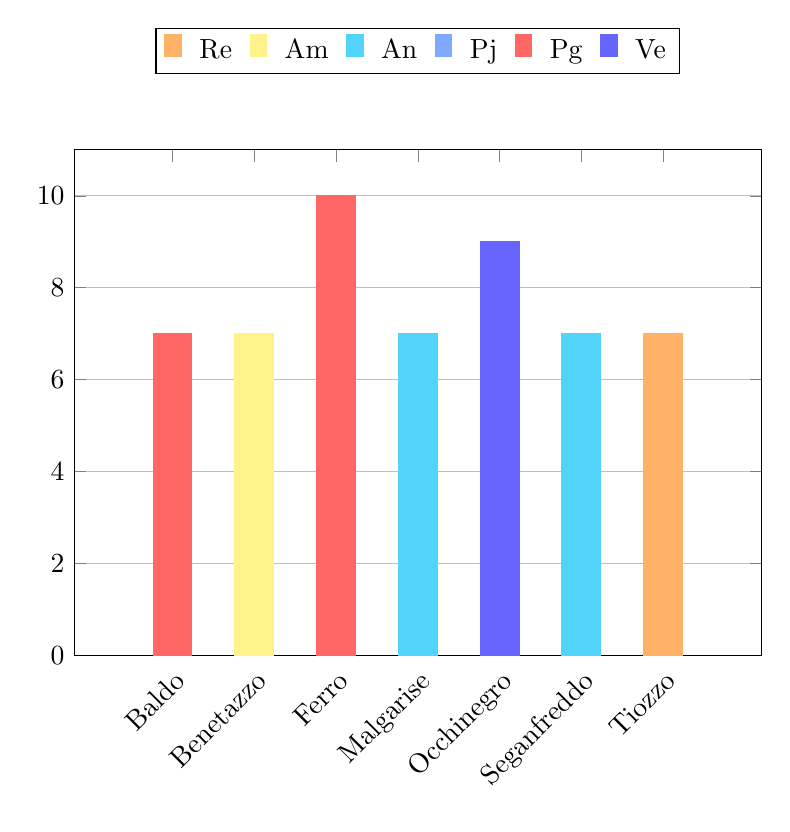
\begin{tikzpicture}
		\begin{axis}[
				width  = 0.85*\textwidth,
				height = 8cm,
				ybar stacked,
				bar width=14pt,
				ymajorgrids = true,
				symbolic x coords={Baldo, Benetazzo, Ferro, Malgarise, Occhinegro, Seganfreddo, Tiozzo},
				xtick = data,
				scaled y ticks = false,
				enlarge x limits=0.2,
				ymin=0,
				legend cell align=left,
				legend style={
						at={(0.5,1.15)},
						anchor=south,
						column sep=1ex,
						legend columns=-1
					},
				xticklabel style={rotate=45, anchor=north east, yshift=0ex, xshift=0ex},
			]
			\addplot+[ybar, resp, fill=resp, mark=none] plot coordinates {
					(Baldo, 0)
					(Benetazzo, 0)
					(Ferro, 0)
					(Malgarise, 0)
					(Occhinegro, 0)
					(Seganfreddo, 0)
					(Tiozzo, 7)
				};
			\addplot+[ybar, amm, fill=amm, mark=none] plot coordinates {
					(Baldo, 0)
					(Benetazzo, 7)
					(Ferro, 0)
					(Malgarise, 0)
					(Occhinegro, 0)
					(Seganfreddo, 0)
					(Tiozzo, 0)
				};
			\addplot+[ybar, an, fill=an, mark=none] plot coordinates {
					(Baldo, 0)
					(Benetazzo, 0)
					(Ferro, 0)
					(Malgarise, 7)
					(Occhinegro, 0)
					(Seganfreddo, 7)
					(Tiozzo, 0)
				};
			\addplot+[ybar, pj, fill=pj, mark=none] plot coordinates {
					(Baldo, 0)
					(Benetazzo, 0)
					(Ferro, 0)
					(Malgarise, 0)
					(Occhinegro, 0)
					(Seganfreddo, 0)
					(Tiozzo, 0)
				};
			\addplot+[ybar, pg, fill=pg, mark=none] plot coordinates {
					(Baldo, 7)
					(Benetazzo, 0)
					(Ferro, 10)
					(Malgarise, 0)
					(Occhinegro, 0)
					(Seganfreddo, 0)
					(Tiozzo, 0)
				};
			\addplot+[ybar, ver, fill=ver, mark=none] plot coordinates {
					(Baldo, 0)
					(Benetazzo, 0)
					(Ferro, 0)
					(Malgarise, 0)
					(Occhinegro, 9)
					(Seganfreddo, 0)
					(Tiozzo, 0)
				};
			\legend{Re, Am, An, Pj, Pg, Ve}
		\end{axis}
	\end{tikzpicture}
	\caption{Impegno preventivo per ruolo dei membri del team durante il primo \href{https://7last.github.io/docs/pb/documentazione-interna/glossario\#sprint}{sprint\textsubscript{G}}}
	
\end{figure}

\newblock
%---------1_GRAFICO A TORTA-----------%
\begin{figure}[!h]
	\centering
	\begin{tikzpicture}
		\def\printonlypositive#1{\ifdim#1pt>0pt#1\%\else\fi}
		\pie[pos={8,0},radius=3.5,text=legend,
			before number=\printonlypositive, after number=, color={resp,amm,an,pj,pg,ver}] {
			13.0/\href{https://7last.github.io/docs/pb/documentazione-interna/glossario\#responsabile}{Responsabile\textsubscript{G}},
			13.0/\href{https://7last.github.io/docs/pb/documentazione-interna/glossario\#amministratore}{Amministratore\textsubscript{G}},
			25.9/\href{https://7last.github.io/docs/pb/documentazione-interna/glossario\#analista}{Analista\textsubscript{G}},
			0.0/\href{https://7last.github.io/docs/pb/documentazione-interna/glossario\#progettista}{Progettista\textsubscript{G}},
			31.5/\href{https://7last.github.io/docs/pb/documentazione-interna/glossario\#programmatore}{Programmatore\textsubscript{G}},
			16.7/\href{https://7last.github.io/docs/pb/documentazione-interna/glossario\#verificatore}{Verificatore\textsubscript{G}}
		}
	\end{tikzpicture}
	\caption{Ripartizione in percentuale dei ruoli nel primo \href{https://7last.github.io/docs/pb/documentazione-interna/glossario\#sprint}{sprint\textsubscript{G}}}
	
\end{figure}

\newpage
\subsubsubsection{Consuntivo}
Le attività previste sono state tutte svolte con successo. Abbiamo completato tutte le richieste della \href{https://7last.github.io/docs/pb/documentazione-interna/glossario\#proponente}{proponente\textsubscript{G}} con anticipo rispetto alla data di fine prevista.

\subsubsubsubsection{Prospetto orario}
\begin{table}[!h]
	\centering
	\begin{tabular}{ | l | c | c | c | c | c | c | c | }
		\hline
		\textbf{}        & \textbf{Re} & \textbf{Am} & \textbf{An} & \textbf{Pj} & \textbf{Pg} & \textbf{Ve} & \textbf{Totale per persona} \\
		\hline
		Baldo            & -           & -           & -           & -           & 7           & -           & 7                           \\
		Benetazzo        & -           & 6           & -           & -           & -           & -           & 6                           \\
		Ferro            & -           & -           & -           & -           & 9           & -           & 9                           \\
		Malgarise        & -           & -           & 6           & -           & -           & -           & 6                           \\
		Occhinegro       & -           & -           & -           & -           & -           & 9           & 9                           \\
		Seganfreddo      & -           & -           & 5,5         & -           & -           & -           & 5,5                         \\
		Tiozzo           & 6,5         & -           & -           & -           & -           & -           & 6,5                         \\
		\hline
		Totale per ruolo & 6,5         & 6           & 11,5        & 0           & 16          & 9           & -                           \\
		\hline
	\end{tabular}
	\caption{Consuntivo orario per ruolo dei membri del team durante il primo \href{https://7last.github.io/docs/pb/documentazione-interna/glossario\#sprint}{sprint\textsubscript{G}}}
	
\end{table}

\subsubsubsubsection{Prospetto economico}
\begin{table}[!h]
	\centering
	\begin{tabular}{ | l | c | c | c | c | c | }
		\hline
		\textbf{Ruolo}             & \textbf{Ore} & \textbf{Costo} & \textbf{Ore rimanenti preventivo} & \textbf{Ore rimanenti consuntivo} \\
		\hline
		\href{https://7last.github.io/docs/pb/documentazione-interna/glossario\#responsabile}{Responsabile\textsubscript{G}}               & 6,5          & 195,00 €       & 49                                & 49,5                              \\
		\href{https://7last.github.io/docs/pb/documentazione-interna/glossario\#amministratore}{Amministratore\textsubscript{G}}             & 6            & 120,00 €       & 49                                & 50                                \\
		\href{https://7last.github.io/docs/pb/documentazione-interna/glossario\#analista}{Analista\textsubscript{G}}                   & 11,5         & 287,50 €       & 64                                & 66,5                              \\
		\href{https://7last.github.io/docs/pb/documentazione-interna/glossario\#progettista}{Progettista\textsubscript{G}}                & 0            & 0,00 €         & 112                               & 112                               \\
		\href{https://7last.github.io/docs/pb/documentazione-interna/glossario\#programmatore}{Programmatore\textsubscript{G}}              & 16           & 240,00 €       & 151                               & 152                               \\
		\href{https://7last.github.io/docs/pb/documentazione-interna/glossario\#verificatore}{Verificatore\textsubscript{G}}               & 9            & 135,00 €       & 165                               & 165                               \\
		\hline
		\textbf{Totale preventivo} & 54           & 1090,00 €      & 590                               & -                                 \\
		\hline
		\textbf{Totale consuntivo} & 49           & 977,50 €       & -                                 & 595                               \\
		\hline
	\end{tabular}
	\caption{Consuntivo economico durante il primo \href{https://7last.github.io/docs/pb/documentazione-interna/glossario\#sprint}{sprint\textsubscript{G}}}
	
\end{table}

\newpage
\subsubsubsubsection{Rischi effettivamente occorsi e loro mitigazione}
\begin{table}[!h]
	\centering
	\begin{tabular}{ | p{6cm} | p{2.5cm} | p{7.5cm} | }
		\hline
		\textbf{Tipologia}                                                       & \textbf{Rischio preventivato} & \textbf{Mitigazione}                                                \\
		\hline
		Inesperienza del team (Rischio \textbf{RT-2}).                           & SI                            & Confronto con gli altri gruppi per la gestione dell'organizzazione. \\
		\hline
		Inesperienza nell'uso delle tecnologie adottate (Rischio \textbf{RT-3}). & SI                            & Autoformazione e discussione interna e con la \href{https://7last.github.io/docs/pb/documentazione-interna/glossario\#proponente}{proponente\textsubscript{G}}.           \\
		\hline
		Ritardi rispetto alle tempistiche previste (Rischio \textbf{RO-3}).      & NO                            & Anticipati alcuni compiti previsti per il prossimo \href{https://7last.github.io/docs/pb/documentazione-interna/glossario\#sprint}{sprint\textsubscript{G}}.          \\
		\hline
	\end{tabular}
	\caption{Rischi effettivamente occorsi e loro mitigazione durante il primo \href{https://7last.github.io/docs/pb/documentazione-interna/glossario\#sprint}{sprint\textsubscript{G}}}
	
\end{table}

\subsubsubsection{Retrospettiva}
La suddivisione iniziale dei ruoli per il presente \href{https://7last.github.io/docs/pb/documentazione-interna/glossario\#sprint}{sprint\textsubscript{G}} si è rivelata efficace e ben pensata. Ciascun componente ha lavorato senza essere sovraccaricato e il lavoro è stato distribuito in modo equo e senza disparità. \\
In seguito alla convocazione per il primo \textit{Diario di Bordo} avvenuta con scarso preavviso e prevista per data e ora in cui era stato pianificato il primo \href{https://7last.github.io/docs/pb/documentazione-interna/glossario\#stato-avanzamento-lavori}{\textit{SAL}\textsubscript{G}} con l'azienda abbiamo dovuto posticipare al 22 aprile l'incontro con la \href{https://7last.github.io/docs/pb/documentazione-interna/glossario\#proponente}{proponente\textsubscript{G}} e questo ha causato un ritardo di 3 giorni inaspettato. Per rimediare a questo ritardo abbiamo iniziato ad effettuare dei progressi sulla documentazione previsti per lo \href{https://7last.github.io/docs/pb/documentazione-interna/glossario\#sprint}{sprint\textsubscript{G}} successivo. \\
Un'ulteriore problematica riscontrata è stata la difficoltà nell'adozione di alcune tecnologie, causando il rallentamento del lavoro. Per il prossimo \href{https://7last.github.io/docs/pb/documentazione-interna/glossario\#sprint}{sprint\textsubscript{G}}, si cercherà di risolvere questo problema con una maggiore formazione e con una maggiore collaborazione tra i membri del gruppo.



\newpage
\subsubsection{Secondo sprint}
\begin{itemize}
	\item Inizio: 2024-04-23
	\item Fine: 2024-05-06
	\item Fine attuale: 2024-05-06
	\item Giorni di ritardo: nessuno
\end{itemize}

\subsubsubsection{Pianificazione}
Durante il secondo periodo, il nostro team si propone di integrare \href{https://7last.github.io/docs/pb/documentazione-interna/glossario\#grafana}{\textit{Grafana}\textsubscript{G}} che rappresenta l'ultimo elemento dello stack tecnologico del \href{https://7last.github.io/docs/pb/documentazione-interna/glossario\#proof-of-concept}{Proof of Concept\textsubscript{G}}, come concordato nel corso del primo \href{https://7last.github.io/docs/pb/documentazione-interna/glossario\#stato-avanzamento-lavori}{SAL\textsubscript{G}}. Inoltre, si prevede l'implementazione della funzionalità di visualizzazione tramite grafici delle misurazioni raccolte,
assieme ad una maggiore persistenza per quanto riguarda i dati raccolti all'interno di \href{https://7last.github.io/docs/pb/documentazione-interna/glossario\#clickhouse}{\textit{ClickHouse}\textsubscript{G}}. \\
Dal punto di vista della documentazione, invece, ci si pone l'obiettivo di portare a compimento il documento \href{https://7last.github.io/docs/pb/documentazione-interna/glossario\#norme-di-progetto}{\textit{Norme di Progetto}\textsubscript{G}}, in modo da avere un quadro chiaro e definito delle regole e delle convenzioni da seguire durante lo sviluppo del progetto. In concomitanza con questa attività, si prosegue con la stesura del \href{https://7last.github.io/docs/pb/documentazione-interna/glossario\#piano-di-progetto}{\textit{Piano di Progetto}\textsubscript{G}}, in particolare con la documentazione del primo e del secondo \href{https://7last.github.io/docs/pb/documentazione-interna/glossario\#sprint}{sprint\textsubscript{G}}, con l'aggiornamento continuo dei documenti \href{https://7last.github.io/docs/pb/documentazione-interna/glossario\#glossario}{\textit{Glossario}\textsubscript{G}} e \href{https://7last.github.io/docs/pb/documentazione-interna/glossario\#piano-di-qualifica}{\textit{Piano di Qualifica}\textsubscript{G}} e, infine, si può procedere con la stesura del documento \href{https://7last.github.io/docs/pb/documentazione-interna/glossario\#analisi-dei-requisiti}{\textit{Analisi dei Requisiti}\textsubscript{G}}, con lo scopo di identificare i casi d'uso fondamentali. \\
Per quanto riguarda gli strumenti adottati, il team prevede di assegnare risorse per l'analisi attenta della tecnologia proposta \href{https://7last.github.io/docs/pb/documentazione-interna/glossario\#redpanda}{\textit{Redpanda}\textsubscript{G}} che andrebbe a sostituire \href{https://7last.github.io/docs/pb/documentazione-interna/glossario\#apache-kafka}{\textit{Apache Kafka}\textsubscript{G}}, consigliata dalla \href{https://7last.github.io/docs/pb/documentazione-interna/glossario\#proponente}{proponente\textsubscript{G}}. Questa fase di valutazione mira a selezionare con attenzione le tecnologie più adatte al compimento delle specifiche del \href{https://7last.github.io/docs/pb/documentazione-interna/glossario\#capitolato}{capitolato\textsubscript{G}}.

\subsubsubsubsection{Rischi attesi}
I rischi attesi per questo periodo sono:
\begin{itemize}
	\item inesperienza nella pianificazione delle attività (RO-1);
	\item impegni personali o universitari (RO-2);
	\item inesperienza nell'uso delle tecnologie adottate (RT-1);
	\item problemi di compatibilità tra le tecnologie adottate (RT-3);
	\item rischio di disaccordi all'interno del gruppo (RC-1).
\end{itemize}
Le differenze rispetto ai rischi attesi nel primo \href{https://7last.github.io/docs/pb/documentazione-interna/glossario\#sprint}{sprint\textsubscript{G}} non sono così significative, questo perché l'esperienza del gruppo è ancora acerba e limitata.
A queste si aggiungono problematiche riguardo agli impegni personali, anche legati alle festività di questo periodo. Infine l'introduzione di \href{https://7last.github.io/docs/pb/documentazione-interna/glossario\#grafana}{\textit{Grafana}\textsubscript{G}},
tecnologia nuova all'interno del team, potrebbe causare problemi di ineseperienza e compatibilità con le tecnologie già adottate.

\subsubsubsection{Preventivo}
Ruoli coinvolti: \href{https://7last.github.io/docs/pb/documentazione-interna/glossario\#responsabile}{Responsabile\textsubscript{G}} (Re), \href{https://7last.github.io/docs/pb/documentazione-interna/glossario\#amministratore}{Amministratore\textsubscript{G}} (Am), \href{https://7last.github.io/docs/pb/documentazione-interna/glossario\#analista}{Analista\textsubscript{G}} (An), \href{https://7last.github.io/docs/pb/documentazione-interna/glossario\#progettista}{Progettista\textsubscript{G}} (Pj), \href{https://7last.github.io/docs/pb/documentazione-interna/glossario\#programmatore}{Programmatore\textsubscript{G}} (Pg), \href{https://7last.github.io/docs/pb/documentazione-interna/glossario\#verificatore}{Verificatore\textsubscript{G}} (Ve).
\begin{table}[!h]
	\centering
	\begin{tabular}{ | l | c | c | c | c | c | c | c | }
		\hline
		\textbf{}        & \textbf{Re} & \textbf{Am} & \textbf{An} & \textbf{Pj} & \textbf{Pg} & \textbf{Ve} & \textbf{Totale per persona} \\
		\hline
		Baldo            & -           & 6           & -           & -           & -           & -           & 6                           \\
		Benetazzo        & -           & -           & -           & -           & -           & 7           & 7                           \\
		Ferro            & -           & -           & 10          & -           & -           & -           & 10                          \\
		Malgarise        & 6           & -           & -           & -           & -           & -           & 6                           \\
		Occhinegro       & -           & -           & -           & -           & 10          & -           & 10                          \\
		Seganfreddo      & -           & -           & -           & 7           & -           & -           & 7                           \\
		Tiozzo           & -           & -           & -           & -           & 10          & -           & 10                          \\
		\hline
		Totale per ruolo & 6           & 6           & 10          & 7           & 20          & 7           & -                           \\
		\hline
	\end{tabular}
	\caption{Preventivo orario per ruolo dei membri del team durante il secondo \href{https://7last.github.io/docs/pb/documentazione-interna/glossario\#sprint}{sprint\textsubscript{G}}}
	
\end{table}

\newpage
%---------1_ISTOGRAMMA-----------%
\begin{figure}[!h]
	\centering
	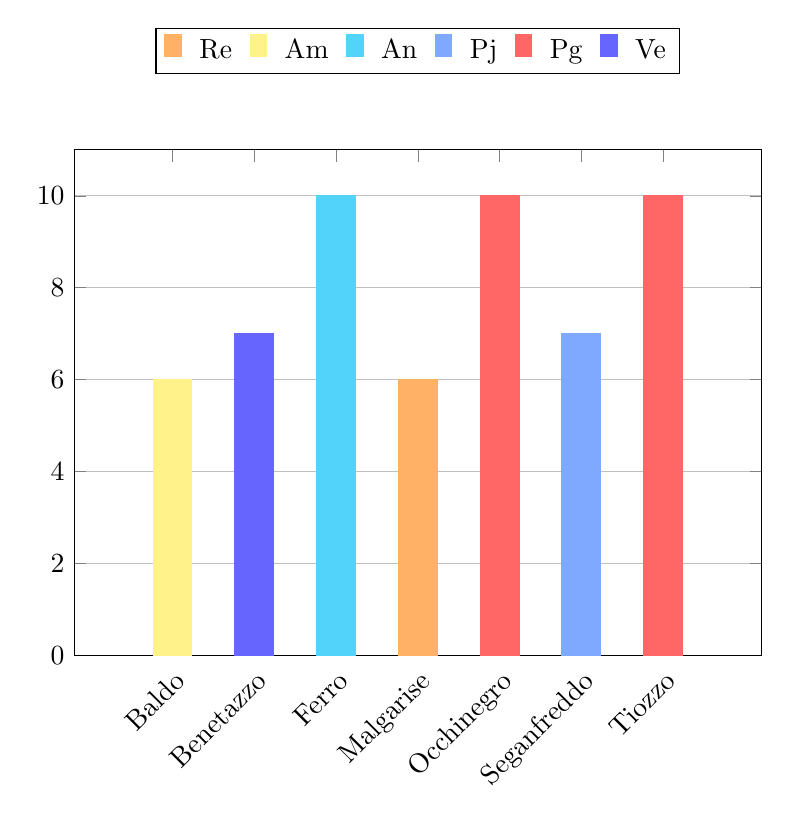
\begin{tikzpicture}
		\begin{axis}[
				width  = 0.85*\textwidth,
				height = 8cm,
				ybar stacked,
				bar width=14pt,
				ymajorgrids = true,
				symbolic x coords={Baldo, Benetazzo, Ferro, Malgarise, Occhinegro, Seganfreddo, Tiozzo},
				xtick = data,
				scaled y ticks = false,
				enlarge x limits=0.2,
				ymin=0,
				legend cell align=left,
				legend style={
						at={(0.5,1.15)},
						anchor=south,
						column sep=1ex,
						legend columns=-1
					},
				xticklabel style={rotate=45, anchor=north east, yshift=0ex, xshift=0ex},
			]
			\addplot+[ybar, resp, fill=resp, mark=none] plot coordinates {
					(Baldo, 0)
					(Benetazzo, 0)
					(Ferro, 0)
					(Malgarise, 6)
					(Occhinegro, 0)
					(Seganfreddo, 0)
					(Tiozzo, 0)
				};
			\addplot+[ybar, amm, fill=amm, mark=none] plot coordinates {
					(Baldo, 6)
					(Benetazzo, 0)
					(Ferro, 0)
					(Malgarise, 0)
					(Occhinegro, 0)
					(Seganfreddo, 0)
					(Tiozzo, 0)
				};
			\addplot+[ybar, an, fill=an, mark=none] plot coordinates {
					(Baldo, 0)
					(Benetazzo, 0)
					(Ferro, 10)
					(Malgarise, 0)
					(Occhinegro, 0)
					(Seganfreddo, 0)
					(Tiozzo, 0)
				};
			\addplot+[ybar, pj, fill=pj, mark=none] plot coordinates {
					(Baldo, 0)
					(Benetazzo, 0)
					(Ferro, 0)
					(Malgarise, 0)
					(Occhinegro, 0)
					(Seganfreddo, 7)
					(Tiozzo, 0)
				};
			\addplot+[ybar, pg, fill=pg, mark=none] plot coordinates {
					(Baldo, 0)
					(Benetazzo, 0)
					(Ferro, 0)
					(Malgarise, 0)
					(Occhinegro, 10)
					(Seganfreddo, 0)
					(Tiozzo, 10)
				};
			\addplot+[ybar, ver, fill=ver, mark=none] plot coordinates {
					(Baldo, 0)
					(Benetazzo, 7)
					(Ferro, 0)
					(Malgarise, 0)
					(Occhinegro, 0)
					(Seganfreddo, 0)
					(Tiozzo, 0)
				};
			\legend{Re, Am, An, Pj, Pg, Ve}
		\end{axis}
	\end{tikzpicture}
	\caption{Impegno preventivo per ruolo dei membri del team durante il secondo \href{https://7last.github.io/docs/pb/documentazione-interna/glossario\#sprint}{sprint\textsubscript{G}}}
	
\end{figure}

%---------1_GRAFICO A TORTA-----------%
\begin{figure}[!h]
	\centering
	\begin{tikzpicture}
		\def\printonlypositive#1{\ifdim#1pt>0pt#1\%\else\fi}
		\pie[pos={8,0},radius=3.5,text=legend,
			before number=\printonlypositive, after number=, color={resp,amm,an,pj,pg,ver}] {
			10.7/\href{https://7last.github.io/docs/pb/documentazione-interna/glossario\#responsabile}{Responsabile\textsubscript{G}},
			10.7/\href{https://7last.github.io/docs/pb/documentazione-interna/glossario\#amministratore}{Amministratore\textsubscript{G}},
			17.9/\href{https://7last.github.io/docs/pb/documentazione-interna/glossario\#analista}{Analista\textsubscript{G}},
			12.5/\href{https://7last.github.io/docs/pb/documentazione-interna/glossario\#progettista}{Progettista\textsubscript{G}},
			35.7/\href{https://7last.github.io/docs/pb/documentazione-interna/glossario\#programmatore}{Programmatore\textsubscript{G}},
			12.5/\href{https://7last.github.io/docs/pb/documentazione-interna/glossario\#verificatore}{Verificatore\textsubscript{G}}
		}
	\end{tikzpicture}
	\caption{Ripartizione in percentuale dei ruoli nel secondo \href{https://7last.github.io/docs/pb/documentazione-interna/glossario\#sprint}{sprint\textsubscript{G}}}
	
\end{figure}

\newpage
\subsubsubsection{Consuntivo}
Tutte le attività previste sono state svolte con successo. Come si può notare dal prospetto orario, i \href{https://7last.github.io/docs/pb/documentazione-interna/glossario\#programmatore}{programmatori\textsubscript{G}} hanno richiesto meno ore rispetto a quanto preventivato.

\subsubsubsubsection{Prospetto orario}
\begin{table}[!h]
	\centering
	\begin{tabular}{ | l | c | c | c | c | c | c | c | }
		\hline
		\textbf{}        & \textbf{Re} & \textbf{Am} & \textbf{An} & \textbf{Pj} & \textbf{Pg} & \textbf{Ve} & \textbf{Totale per persona} \\
		\hline
		Baldo            & -           & 6           & -           & -           & -           & -           & 6                           \\
		Benetazzo        & -           & -           & -           & -           & -           & 6           & 6                           \\
		Ferro            & -           & -           & 10          & -           & -           & -           & 10                          \\
		Malgarise        & 5           & -           & -           & -           & -           & -           & 5                           \\
		Occhinegro       & -           & -           & -           & -           & 9           & -           & 9                           \\
		Seganfreddo      & -           & -           & -           & 7           & -           & -           & 7                           \\
		Tiozzo           & -           & -           & -           & -           & 9           & -           & 9                           \\
		\hline
		Totale per ruolo & 5           & 6           & 10          & 7           & 18          & 6           & -                           \\
		\hline
	\end{tabular}
	\caption{Consuntivo orario per ruolo dei membri del team durante il secondo \href{https://7last.github.io/docs/pb/documentazione-interna/glossario\#sprint}{sprint\textsubscript{G}}}
	
\end{table}

\subsubsubsubsection{Prospetto economico}
\begin{table}[!h]
	\centering
	\begin{tabular}{ | l | c | c | c | c | c | }
		\hline
		\textbf{Ruolo}             & \textbf{Ore} & \textbf{Costo} & \textbf{Ore rimanenti preventivo} & \textbf{Ore rimanenti consuntivo} \\
		\hline
		\href{https://7last.github.io/docs/pb/documentazione-interna/glossario\#responsabile}{Responsabile\textsubscript{G}}               & 5            & 150,00 €       & 43,5                              & 44,5                              \\
		\href{https://7last.github.io/docs/pb/documentazione-interna/glossario\#amministratore}{Amministratore\textsubscript{G}}             & 6            & 120,00 €       & 44                                & 44                                \\
		\href{https://7last.github.io/docs/pb/documentazione-interna/glossario\#analista}{Analista\textsubscript{G}}                   & 10           & 250,00 €       & 56,5                              & 56,5                              \\
		\href{https://7last.github.io/docs/pb/documentazione-interna/glossario\#progettista}{Progettista\textsubscript{G}}                & 7            & 175,00 €       & 105                               & 105                               \\
		\href{https://7last.github.io/docs/pb/documentazione-interna/glossario\#programmatore}{Programmatore\textsubscript{G}}              & 18           & 270,00 €       & 132                               & 134                               \\
		\href{https://7last.github.io/docs/pb/documentazione-interna/glossario\#verificatore}{Verificatore\textsubscript{G}}               & 6            & 90,00 €        & 158                               & 159                               \\
		\hline
		\textbf{Totale preventivo} & 56           & 1130,00 €      & 539                               & -                                 \\
		\hline
		\textbf{Totale consuntivo} & 52           & 1055,00 €      & -                                 & 543                               \\
		\hline
	\end{tabular}
	\caption{Prospetto economico consuntivo durante il secondo \href{https://7last.github.io/docs/pb/documentazione-interna/glossario\#sprint}{sprint\textsubscript{G}}}
	
\end{table}

\newpage
\subsubsubsubsection{Rischi effettivamente occorsi e loro mitigazione}
\begin{table}[h]
	\centering
	\begin{tabular}{ | p{6cm} | p{2.5cm} | p{7.5cm} | }
		\hline
		\textbf{Tipologia}                                                       & \textbf{Rischio preventivato} & \textbf{Mitigazione}                                                               \\
		\hline
		Inesperienza del team (Rischio \textbf{RO-1}).                           & SI                            & Ridistribuzione compiti assegnati durante lo \href{https://7last.github.io/docs/pb/documentazione-interna/glossario\#sprint}{sprint\textsubscript{G}}.                               \\
		\hline
		Impegni personali o universitari (Rischio \textbf{RO-2}).                & NO                            & Comunicato in anticipo gli impegni, lavoro affidato svolto prima o dopo l'impegno. \\
		\hline
		Inesperienza nell'uso delle tecnologie adottate (Rischio \textbf{RT-3}). & SI                            & Autoformazione e pair programming.                                                 \\
		\hline
	\end{tabular}
	\caption{Rischi effettivamente occorsi e loro mitigazione durante il secondo \href{https://7last.github.io/docs/pb/documentazione-interna/glossario\#sprint}{sprint\textsubscript{G}}}
	
\end{table}

\subsubsubsection{Retrospettiva}
La suddivisione dei compiti da svolgere non è stata ottimale, in quanto alcuni membri del team hanno completato le attività assegnate in anticipo rispetto alla data di fine prevista, mentre altri hanno richiesto più tempo del previsto. Per i prossimi \href{https://7last.github.io/docs/pb/documentazione-interna/glossario\#sprint}{sprint\textsubscript{G}} valuteremo soluzioni alternative per evitare che ciò accada nuovamente. \\
Alcuni membri del gruppo hanno avuto impegni personali imprevisti durante questo periodo che hanno portato via del tempo prezioso per il completamento delle attività previste. Tali impegni sono stati comunicati tempestivamente al team e i compiti assegnati sono stati completati prima o dopo l'impegno. \\
Permane la difficoltà nell'uso delle tecnologie previste. In seguito alla turnazione dei ruoli altri membri del team si sono ritrovati a dover affrontare le stesse difficoltà avute dai colleghi in precedenza. In questo caso le difficoltà avute sono state superate mediante attività di autoformazione e \textit{pair programming} assieme ai compagni che avevano risolto gli stessi problemi nello \href{https://7last.github.io/docs/pb/documentazione-interna/glossario\#sprint}{sprint\textsubscript{G}} precedente.



\newpage
\subsubsection{Terzo sprint}
\begin{itemize}
	\item Inizio: 2024-05-07
	\item Fine: 2024-05-15
	\item Fine attuale: 2024-05-15
	\item Giorni di ritardo: nessuno
\end{itemize}

\subsubsubsection{Pianificazione}
In questo periodo il gruppo si concentrerà ad analizzare le possibilità di miglioramento suggerite dall' azienda per quanto riguarda la visualizzazione dei dati in \href{https://7last.github.io/docs/pb/documentazione-interna/glossario\#grafana}{\textit{Grafana}\textsubscript{G}}. Molte risorse saranno ancora dedicate alla documentazione, in particolare al documento \href{https://7last.github.io/docs/pb/documentazione-interna/glossario\#analisi-dei-requisiti}{\textit{Analisi dei Requisiti}\textsubscript{G}} e \href{https://7last.github.io/docs/pb/documentazione-interna/glossario\#piano-di-progetto}{\textit{Piano di Progetto}\textsubscript{G}}. \\
Durante il \href{https://7last.github.io/docs/pb/documentazione-interna/glossario\#stato-avanzamento-lavori}{\textit{SAL}\textsubscript{G}} del precedente \href{https://7last.github.io/docs/pb/documentazione-interna/glossario\#sprint}{sprint\textsubscript{G}} sono stati fissati con l'azienda i seguenti obiettivi:
\begin{itemize}
	\item correzione della visualizzazione di latitudine e longitudine (con tutti i decimali);
	\item aggiunta di filtri per migliorare la visualizzazione dei dati, anche per poter visualizzare quelli di un singolo \href{https://7last.github.io/docs/pb/documentazione-interna/glossario\#sensore}{sensore\textsubscript{G}};
	\item rendere più chiaro il grafico \textit{Daily mean};
	\item togliere il grafico \textit{Average temperature per minute} o sostituirlo con un grafico più significativo;
	\item raffinamento globale della \href{https://7last.github.io/docs/pb/documentazione-interna/glossario\#dashboard}{dashboard\textsubscript{G}}.
\end{itemize}

\subsubsubsubsection{Rischi attesi}
I rischi attesi per questo periodo sono:
\begin{itemize}
	\item inesperienza del team nella pianificazione delle attività (RO-1);
	\item ritardi rispetto alle tempistiche previste (RO-3);
	\item inesperienza nell'uso delle tecnologie adottate (RT-1).
\end{itemize}
Siamo ancora nelle fasi iniziali del progetto, dobbiamo ancora imparare come pianificare le attività al meglio; inoltre molti membri del gruppo non hanno mai usato le tecnologie previste.

\subsubsubsection{Preventivo}
Ruoli coinvolti: \href{https://7last.github.io/docs/pb/documentazione-interna/glossario\#responsabile}{Responsabile\textsubscript{G}} (Re), \href{https://7last.github.io/docs/pb/documentazione-interna/glossario\#amministratore}{Amministratore\textsubscript{G}} (Am), \href{https://7last.github.io/docs/pb/documentazione-interna/glossario\#analista}{Analista\textsubscript{G}} (An), \href{https://7last.github.io/docs/pb/documentazione-interna/glossario\#progettista}{Progettista\textsubscript{G}} (Pj), \href{https://7last.github.io/docs/pb/documentazione-interna/glossario\#programmatore}{Programmatore\textsubscript{G}} (Pg), \href{https://7last.github.io/docs/pb/documentazione-interna/glossario\#verificatore}{Verificatore\textsubscript{G}} (Ve).
\begin{table}[!h]
	\centering
	\begin{tabular}{ | l | c | c | c | c | c | c | c | }
		\hline
		\textbf{}        & \textbf{Re} & \textbf{Am} & \textbf{An} & \textbf{Pj} & \textbf{Pg} & \textbf{Ve} & \textbf{Totale per persona} \\
		\hline
		Baldo            & -           & -           & -           & -           & -           & 4           & 4                           \\
		Benetazzo        & 4           & -           & -           & -           & -           & -           & 4                           \\
		Ferro            & -           & -           & -           & 5           & -           & -           & 5                           \\
		Malgarise        & -           & -           & -           & -           & 5           & -           & 5                           \\
		Occhinegro       & -           & -           & 6           & -           & -           & -           & 6                           \\
		Seganfreddo      & -           & -           & -           & -           & 5           & -           & 5                           \\
		Tiozzo           & -           & 5           & -           & -           & -           & -           & 5                           \\
		\hline
		Totale per ruolo & 4           & 5           & 6           & 5           & 10          & 4           & -                           \\
		\hline
	\end{tabular}
	\caption{Preventivo orario per ruolo dei membri del team durante il terzo \href{https://7last.github.io/docs/pb/documentazione-interna/glossario\#sprint}{sprint\textsubscript{G}}}
	
\end{table}

%---------1_ISTOGRAMMA-----------%
\begin{figure}[!h]
	\centering
	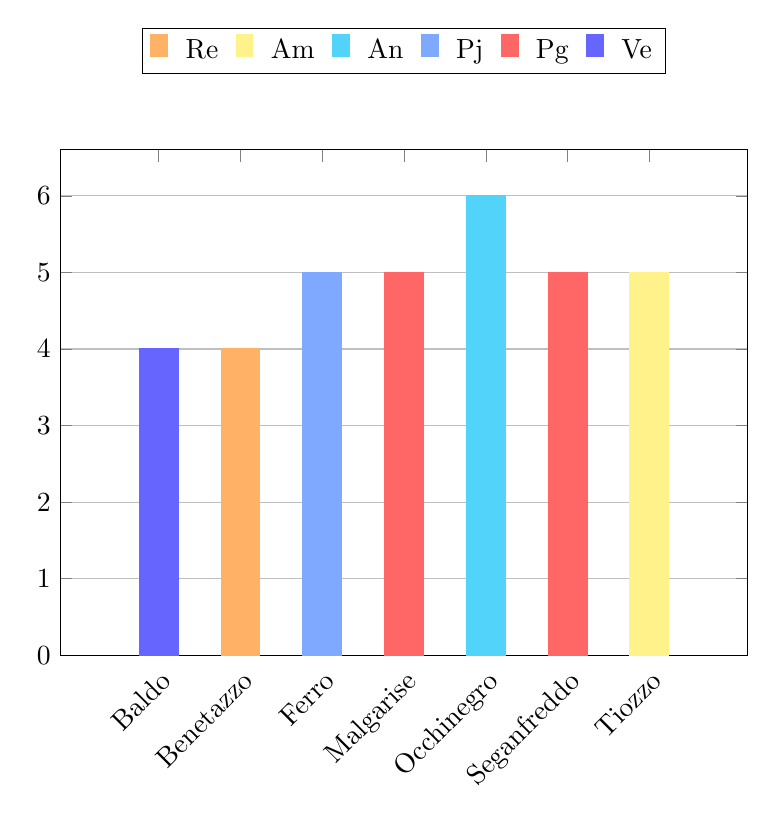
\begin{tikzpicture}
		\begin{axis}[
				width  = 0.85*\textwidth,
				height = 8cm,
				ybar stacked,
				bar width=14pt,
				ymajorgrids = true,
				symbolic x coords={Baldo, Benetazzo, Ferro, Malgarise, Occhinegro, Seganfreddo, Tiozzo},
				xtick = data,
				scaled y ticks = false,
				enlarge x limits=0.2,
				ymin=0,
				legend cell align=left,
				legend style={
						at={(0.5,1.15)},
						anchor=south,
						column sep=1ex,
						legend columns=-1
					},
				xticklabel style={rotate=45, anchor=north east, yshift=0ex, xshift=0ex},
			]
			\addplot+[ybar, resp, fill=resp, mark=none] plot coordinates {
					(Baldo, 0)
					(Benetazzo, 4)
					(Ferro, 0)
					(Malgarise, 0)
					(Occhinegro, 0)
					(Seganfreddo, 0)
					(Tiozzo, 0)
				};
			\addplot+[ybar, amm, fill=amm, mark=none] plot coordinates {
					(Baldo, 0)
					(Benetazzo, 0)
					(Ferro, 0)
					(Malgarise, 0)
					(Occhinegro, 0)
					(Seganfreddo, 0)
					(Tiozzo, 5)
				};
			\addplot+[ybar, an, fill=an, mark=none] plot coordinates {
					(Baldo, 0)
					(Benetazzo, 0)
					(Ferro, 0)
					(Malgarise, 0)
					(Occhinegro, 6)
					(Seganfreddo, 0)
					(Tiozzo, 0)
				};
			\addplot+[ybar, pj, fill=pj, mark=none] plot coordinates {
					(Baldo, 0)
					(Benetazzo, 0)
					(Ferro, 5)
					(Malgarise, 0)
					(Occhinegro, 0)
					(Seganfreddo, 0)
					(Tiozzo, 0)
				};
			\addplot+[ybar, pg, fill=pg, mark=none] plot coordinates {
					(Baldo, 0)
					(Benetazzo, 0)
					(Ferro, 0)
					(Malgarise, 5)
					(Occhinegro, 0)
					(Seganfreddo, 5)
					(Tiozzo, 0)
				};
			\addplot+[ybar, ver, fill=ver, mark=none] plot coordinates {
					(Baldo, 4)
					(Benetazzo, 0)
					(Ferro, 0)
					(Malgarise, 0)
					(Occhinegro, 0)
					(Seganfreddo, 0)
					(Tiozzo, 0)
				};
			\legend{Re, Am, An, Pj, Pg, Ve}
		\end{axis}
	\end{tikzpicture}
	\caption{Impegno preventivo per ruolo dei membri del team durante il terzo \href{https://7last.github.io/docs/pb/documentazione-interna/glossario\#sprint}{sprint\textsubscript{G}}}
	
\end{figure}

\newblock
%---------1_GRAFICO A TORTA-----------%
\begin{figure}[!h]
	\centering
	\begin{tikzpicture}
		\def\printonlypositive#1{\ifdim#1pt>0pt#1\%\else\fi}
		\pie[pos={8,0},radius=3.5,text=legend,
			before number=\printonlypositive, after number=, color={resp,amm,an,pj,pg,ver}] {
			11.8/\href{https://7last.github.io/docs/pb/documentazione-interna/glossario\#responsabile}{Responsabile\textsubscript{G}},
			14.7/\href{https://7last.github.io/docs/pb/documentazione-interna/glossario\#amministratore}{Amministratore\textsubscript{G}},
			17.6/\href{https://7last.github.io/docs/pb/documentazione-interna/glossario\#analista}{Analista\textsubscript{G}},
			14.7/\href{https://7last.github.io/docs/pb/documentazione-interna/glossario\#progettista}{Progettista\textsubscript{G}},
			29.4/\href{https://7last.github.io/docs/pb/documentazione-interna/glossario\#programmatore}{Programmatore\textsubscript{G}},
			11.8/\href{https://7last.github.io/docs/pb/documentazione-interna/glossario\#verificatore}{Verificatore\textsubscript{G}}
		}
	\end{tikzpicture}
	\caption{Ripartizione in percentuale dei ruoli nel terzo \href{https://7last.github.io/docs/pb/documentazione-interna/glossario\#sprint}{sprint\textsubscript{G}}}
	
\end{figure}

\subsubsubsection{Consuntivo}
Anche per questo \href{https://7last.github.io/docs/pb/documentazione-interna/glossario\#sprint}{sprint\textsubscript{G}}, nonostante la durata ridotta, siamo riusciti a portare a termine tutte le attività previste.

\subsubsubsubsection{Prospetto orario}
\begin{table}[!h]
	\centering
	\begin{tabular}{ | l | c | c | c | c | c | c | c | }
		\hline
		\textbf{}        & \textbf{Re} & \textbf{Am} & \textbf{An} & \textbf{Pj} & \textbf{Pg} & \textbf{Ve} & \textbf{Totale per persona} \\
		\hline
		Baldo            & -           & -           & -           & -           & -           & 4,5         & 4,5                         \\
		Benetazzo        & 4,5         & -           & -           & -           & -           & -           & 4,5                         \\
		Ferro            & -           & -           & -           & 5           & -           & -           & 4                           \\
		Malgarise        & -           & -           & -           & -           & 6           & -           & 6                           \\
		Occhinegro       & -           & -           & 6,5         & -           & -           & -           & 6,5                         \\
		Seganfreddo      & -           & -           & -           & -           & 7           & -           & 7                           \\
		Tiozzo           & -           & 5           & -           & -           & -           & -           & 5                           \\
		\hline
		Totale per ruolo & 4,5         & 5           & 6,5         & 4           & 13          & 4,5         & -                           \\
		\hline
	\end{tabular}
	\caption{Consuntivo orario per ruolo dei membri del team durante il terzo \href{https://7last.github.io/docs/pb/documentazione-interna/glossario\#sprint}{sprint\textsubscript{G}}}
	
\end{table}

\subsubsubsubsection{Prospetto economico}
\begin{table}[!h]
	\centering
	\begin{tabular}{ | l | c | c | c | c | c | }
		\hline
		\textbf{Ruolo}             & \textbf{Ore} & \textbf{Costo} & \textbf{Ore rimanenti preventivo} & \textbf{Ore rimanenti consuntivo} \\
		\hline
		\href{https://7last.github.io/docs/pb/documentazione-interna/glossario\#responsabile}{Responsabile\textsubscript{G}}               & 4,5          & 135,00 €       & 40,5                              & 40                                \\
		\href{https://7last.github.io/docs/pb/documentazione-interna/glossario\#amministratore}{Amministratore\textsubscript{G}}             & 5            & 100,00 €       & 39                                & 39                                \\
		\href{https://7last.github.io/docs/pb/documentazione-interna/glossario\#analista}{Analista\textsubscript{G}}                   & 6,5          & 162,50 €       & 50,5                              & 50                                \\
		\href{https://7last.github.io/docs/pb/documentazione-interna/glossario\#progettista}{Progettista\textsubscript{G}}                & 4            & 100,00 €       & 100                               & 101                               \\
		\href{https://7last.github.io/docs/pb/documentazione-interna/glossario\#programmatore}{Programmatore\textsubscript{G}}              & 13           & 195,00 €       & 124                               & 121                               \\
		\href{https://7last.github.io/docs/pb/documentazione-interna/glossario\#verificatore}{Verificatore\textsubscript{G}}               & 4,5          & 67,50 €        & 155                               & 154,5                             \\
		\hline
		\textbf{Totale preventivo} & 34           & 705,00 €       & 509                               & -                                 \\
		\hline
		\textbf{Totale consuntivo} & 37,5         & 760,00 €       & -                                 & 505,5                             \\
		\hline
	\end{tabular}
	\caption{Prospetto economico consuntivo durante il terzo \href{https://7last.github.io/docs/pb/documentazione-interna/glossario\#sprint}{sprint\textsubscript{G}}}
	
\end{table}

\subsubsubsubsection{Rischi effettivamente occorsi e loro mitigazione}
\begin{table}[!h]
	\centering
	\begin{tabular}{ | p{6cm} | p{2.5cm} | p{7.5cm} | }
		\hline
		\textbf{Tipologia}                                                      & \textbf{Rischio preventivato} & \textbf{Mitigazione}               \\
		\hline
		Inesperienza nell'uso delle tecnologie adottate (Rischio \textbf{RT-3}) & SI                            & Autoformazione e pair programming. \\
		\hline
	\end{tabular}
	\caption{Rischi effettivamente occorsi e loro mitigazione durante il terzo \href{https://7last.github.io/docs/pb/documentazione-interna/glossario\#sprint}{sprint\textsubscript{G}}}
	
\end{table}

\subsubsubsection{Retrospettiva}
Durante l'ultimo \href{https://7last.github.io/docs/pb/documentazione-interna/glossario\#stato-avanzamento-lavori}{\textit{SAL}\textsubscript{G}} con l'azienda abbiamo deciso su loro consiglio di accorciare gli \href{https://7last.github.io/docs/pb/documentazione-interna/glossario\#sprint}{sprint\textsubscript{G}}, passando dalla durata di due settimane a quella di una settimana. Abbiamo anche deciso di spostare i prossimi al mercoledì, in quanto uno dei membri del gruppo era impossibilitato a partecipare il lunedì per impegni di lavoro. Questo ci ha permesso di avere due giorni in più in questo \href{https://7last.github.io/docs/pb/documentazione-interna/glossario\#sprint}{sprint\textsubscript{G}} e di attenuare l'impatto del cambiamento di durata. Per evitare ritardi, però, si è reso necessario riorganizzare le attività inizialmente pianificate in modo errato, portando ad un maggior consumo di ore produttive da parte dei \href{https://7last.github.io/docs/pb/documentazione-interna/glossario\#programmatore}{programmatori\textsubscript{G}} in particolare, e quindi ad una spesa superiore a quanto preventivato. \\
Permane la difficoltà nell'uso delle tecnologie adottate. In particolare abbiamo riscontrato in questo \href{https://7last.github.io/docs/pb/documentazione-interna/glossario\#sprint}{sprint\textsubscript{G}} diverse difficoltà nella configurazione di tali strumenti in diversi sistemi operativi. Come già sperimentato nel precedente \href{https://7last.github.io/docs/pb/documentazione-interna/glossario\#sprint}{sprint\textsubscript{G}} le attività di autoformazione e \textit{pair programming} si sono rivelate molto efficaci per superare tali difficoltà ed evitare ritardi nel completamento delle attività.



\newpage
\subsubsection{Quarto sprint}
\begin{itemize}
	\item Inizio: 2024-05-16
	\item Fine: 2024-05-22
	\item Fine attuale: 2024-05-22
	\item Giorni di ritardo: nessuno
\end{itemize}

\subsubsubsection{Pianificazione}
In questo periodo il gruppo si impegna ad implementare le migliorie suggerite.
In particolare ci si concentrerà su:
\begin{itemize}
	\item aggiunta di una o più \textit{query di aggregazione}, in particolare fare delle \href{https://7last.github.io/docs/pb/documentazione-interna/glossario\#dashboard}{dashboard\textsubscript{G}} analitiche in cui si
	      mostrano andamenti e report;
	\item aggiunta di ulteriori sensori dislocati in luoghi e distanze differenti;
	\item miglioramenti generali alla \href{https://7last.github.io/docs/pb/documentazione-interna/glossario\#dashboard}{dashboard\textsubscript{G}}.
\end{itemize}

\subsubsubsubsection{Rischi attesi}
I rischi attesi per questo periodo sono:
\begin{itemize}
	\item impegni personali o universitari (RO-2);
	\item inesperienza nell'uso delle tecnologie adottate (RT-1);
	\item problemi di compatibilità tra le tecnologie adottate (RT-3);
	\item rischio di conflitti interni (RC-1).
\end{itemize}
Il rischio dell'inesperienza nell'uso delle tecnologie adottate (\textbf{RT-1}) è ancora presente ma in parte mitigato visto che uno dei
due \href{https://7last.github.io/docs/pb/documentazione-interna/glossario\#programmatore}{programmatori\textsubscript{G}} ha già lavorato con le tecnologie adottate.
\newpage
\subsubsubsection{Preventivo}
Ruoli coinvolti: \href{https://7last.github.io/docs/pb/documentazione-interna/glossario\#responsabile}{Responsabile\textsubscript{G}} (Re), \href{https://7last.github.io/docs/pb/documentazione-interna/glossario\#amministratore}{Amministratore\textsubscript{G}} (Am), \href{https://7last.github.io/docs/pb/documentazione-interna/glossario\#analista}{Analista\textsubscript{G}} (An), \href{https://7last.github.io/docs/pb/documentazione-interna/glossario\#progettista}{Progettista\textsubscript{G}} (Pj), \href{https://7last.github.io/docs/pb/documentazione-interna/glossario\#programmatore}{Programmatore\textsubscript{G}} (Pg), \href{https://7last.github.io/docs/pb/documentazione-interna/glossario\#verificatore}{Verificatore\textsubscript{G}} (Ve).
\begin{table}[!h]
	\centering
	\begin{tabular}{ | l | c | c | c | c | c | c | c | }
		\hline
		\textbf{}        & \textbf{Re} & \textbf{Am} & \textbf{An} & \textbf{Pj} & \textbf{Pg} & \textbf{Ve} & \textbf{Totale per persona} \\
		\hline
		Baldo            & -           & -           & 5           & -           & -           & -           & 5                           \\
		Benetazzo        & -           & -           & -           & -           & 4           & -           & 4                           \\
		Ferro            & -           & -           & -           & -           & 4           & -           & 4                           \\
		Malgarise        & -           & -           & -           & 4           & -           & -           & 4                           \\
		Occhinegro       & 4           & -           & -           & -           & -           & -           & 4                           \\
		Seganfreddo      & -           & 4           & -           & -           & -           & -           & 4                           \\
		Tiozzo           & -           & -           & -           & -           & -           & 7           & 7                           \\
		\hline
		Totale per ruolo & 4           & 4           & 5           & 4           & 8           & 7           & -                           \\
		\hline
	\end{tabular}
	\caption{Preventivo orario per ruolo dei membri del team durante il quarto \href{https://7last.github.io/docs/pb/documentazione-interna/glossario\#sprint}{sprint\textsubscript{G}}}
	
\end{table}

%---------1_ISTOGRAMMA-----------%
\begin{figure}[!h]
	\centering
	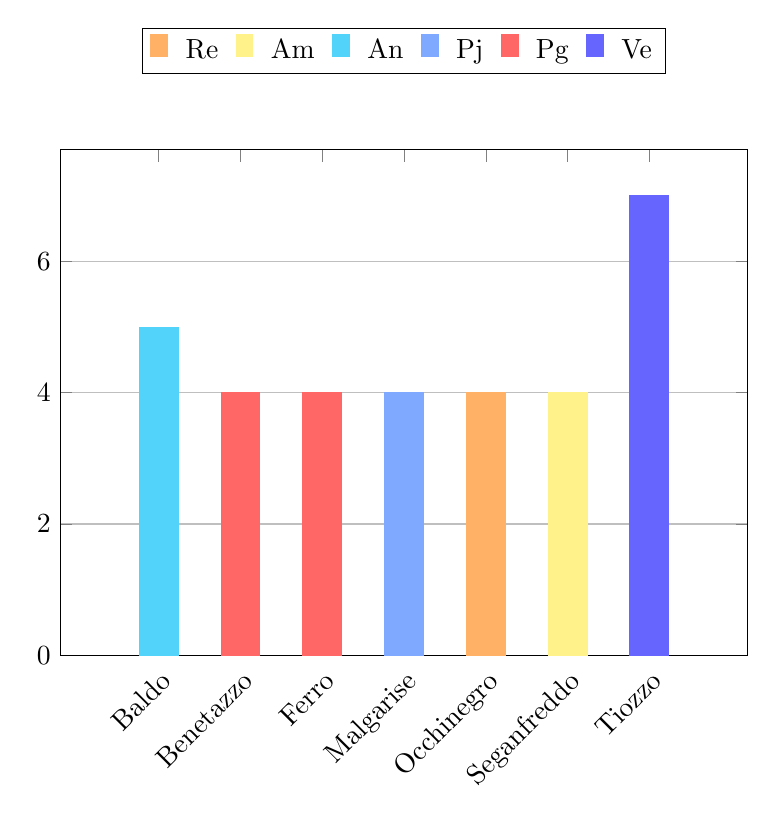
\begin{tikzpicture}
		\begin{axis}[
				width  = 0.85*\textwidth,
				height = 8cm,
				ybar stacked,
				bar width=14pt,
				ymajorgrids = true,
				symbolic x coords={Baldo, Benetazzo, Ferro, Malgarise, Occhinegro, Seganfreddo, Tiozzo},
				xtick = data,
				scaled y ticks = false,
				enlarge x limits=0.2,
				ymin=0,
				legend cell align=left,
				legend style={
						at={(0.5,1.15)},
						anchor=south,
						column sep=1ex,
						legend columns=-1
					},
				xticklabel style={rotate=45, anchor=north east, yshift=0ex, xshift=0ex},
			]
			\addplot+[ybar, resp, fill=resp, mark=none] plot coordinates {
					(Baldo, 0)
					(Benetazzo, 0)
					(Ferro, 0)
					(Malgarise, 0)
					(Occhinegro, 4)
					(Seganfreddo, 0)
					(Tiozzo, 0)
				};
			\addplot+[ybar, amm, fill=amm, mark=none] plot coordinates {
					(Baldo, 0)
					(Benetazzo, 0)
					(Ferro, 0)
					(Malgarise, 0)
					(Occhinegro, 0)
					(Seganfreddo, 4)
					(Tiozzo, 0)
				};
			\addplot+[ybar, an, fill=an, mark=none] plot coordinates {
					(Baldo, 5)
					(Benetazzo, 0)
					(Ferro, 0)
					(Malgarise, 0)
					(Occhinegro, 0)
					(Seganfreddo, 0)
					(Tiozzo, 0)
				};
			\addplot+[ybar, pj, fill=pj, mark=none] plot coordinates {
					(Baldo, 0)
					(Benetazzo, 0)
					(Ferro, 0)
					(Malgarise, 4)
					(Occhinegro, 0)
					(Seganfreddo, 0)
					(Tiozzo, 0)
				};
			\addplot+[ybar, pg, fill=pg, mark=none] plot coordinates {
					(Baldo, 0)
					(Benetazzo, 4)
					(Ferro, 4)
					(Malgarise, 0)
					(Occhinegro, 0)
					(Seganfreddo, 0)
					(Tiozzo, 0)
				};
			\addplot+[ybar, ver, fill=ver, mark=none] plot coordinates {
					(Baldo, 0)
					(Benetazzo, 0)
					(Ferro, 0)
					(Malgarise, 0)
					(Occhinegro, 0)
					(Seganfreddo, 0)
					(Tiozzo, 7)
				};
			\legend{Re, Am, An, Pj, Pg, Ve}
		\end{axis}
	\end{tikzpicture}
	\caption{Impegno preventivo per ruolo dei membri del team durante il quarto \href{https://7last.github.io/docs/pb/documentazione-interna/glossario\#sprint}{sprint\textsubscript{G}}}
	
\end{figure}

%---------1_GRAFICO A TORTA-----------%
\begin{figure}[!h]
	\centering
	\begin{tikzpicture}
		\def\printonlypositive#1{\ifdim#1pt>0pt
				#1
			\fi}
		\pie[pos={8,0},radius=3.5,text=legend,
			before number=\printonlypositive,color={resp,amm,an,pj,pg,ver}] {
			12.5/\href{https://7last.github.io/docs/pb/documentazione-interna/glossario\#responsabile}{Responsabile\textsubscript{G}},
			12.5/\href{https://7last.github.io/docs/pb/documentazione-interna/glossario\#amministratore}{Amministratore\textsubscript{G}},
			15.6/\href{https://7last.github.io/docs/pb/documentazione-interna/glossario\#analista}{Analista\textsubscript{G}},
			12.5/\href{https://7last.github.io/docs/pb/documentazione-interna/glossario\#progettista}{Progettista\textsubscript{G}},
			25.0/\href{https://7last.github.io/docs/pb/documentazione-interna/glossario\#programmatore}{Programmatore\textsubscript{G}},
			21.9/\href{https://7last.github.io/docs/pb/documentazione-interna/glossario\#verificatore}{Verificatore\textsubscript{G}}
		}
	\end{tikzpicture}
	\caption{Ripartizione in percentuale dei ruoli nel quarto \href{https://7last.github.io/docs/pb/documentazione-interna/glossario\#sprint}{sprint\textsubscript{G}}}
	
\end{figure}

\newpage
\subsubsubsection{Consuntivo}
In questo \href{https://7last.github.io/docs/pb/documentazione-interna/glossario\#sprint}{sprint\textsubscript{G}} siamo riusciti a portare a termine tutte le attività previste.

\subsubsubsubsection{Prospetto orario}
\begin{table}[!h]
	\centering
	\begin{tabular}{ | l | c | c | c | c | c | c | c | }
		\hline
		\textbf{}        & \textbf{Re} & \textbf{Am} & \textbf{An} & \textbf{Pj} & \textbf{Pg} & \textbf{Ve} & \textbf{Totale per persona} \\
		\hline
		Baldo            & -           & -           & 5           & -           & -           & -           & 5                           \\
		Benetazzo        & -           & -           & -           & -           & 4           & -           & 4                           \\
		Ferro            & -           & -           & -           & -           & 4           & -           & 4                           \\
		Malgarise        & -           & -           & -           & 4           & -           & -           & 4                           \\
		Occhinegro       & 3           & -           & -           & -           & -           & -           & 3                           \\
		Seganfreddo      & -           & 4           & -           & -           & -           & -           & 4                           \\
		Tiozzo           & -           & -           & -           & -           & -           & 7           & 7                           \\
		\hline
		Totale per ruolo & 3           & 4           & 5           & 4           & 8           & 7           & -                           \\
		\hline
	\end{tabular}
	\caption{Consuntivo orario per ruolo dei membri del team durante il quarto \href{https://7last.github.io/docs/pb/documentazione-interna/glossario\#sprint}{sprint\textsubscript{G}}}
	
\end{table}
\newpage
\subsubsubsubsection{Prospetto economico}
\begin{table}[!h]
	\centering
	\begin{tabular}{ | l | c | c | c | c | c | }
		\hline
		\textbf{Ruolo}             & \textbf{Ore} & \textbf{Costo} & \textbf{Ore rimanenti preventivo} & \textbf{Ore rimanenti consuntivo} \\
		\hline
		\href{https://7last.github.io/docs/pb/documentazione-interna/glossario\#responsabile}{Responsabile\textsubscript{G}}               & 3            & 90,00 €        & 36                                & 37                                \\
		\href{https://7last.github.io/docs/pb/documentazione-interna/glossario\#amministratore}{Amministratore\textsubscript{G}}             & 4            & 80,00 €        & 35                                & 35                                \\
		\href{https://7last.github.io/docs/pb/documentazione-interna/glossario\#analista}{Analista\textsubscript{G}}                   & 5            & 125,00 €       & 45                                & 45                                \\
		\href{https://7last.github.io/docs/pb/documentazione-interna/glossario\#progettista}{Progettista\textsubscript{G}}                & 4            & 100,00 €       & 97                                & 97                                \\
		\href{https://7last.github.io/docs/pb/documentazione-interna/glossario\#programmatore}{Programmatore\textsubscript{G}}              & 8            & 120,00 €       & 113                               & 113                               \\
		\href{https://7last.github.io/docs/pb/documentazione-interna/glossario\#verificatore}{Verificatore\textsubscript{G}}               & 7            & 105,00 €       & 147,5                             & 147,5                             \\
		\hline
		\textbf{Totale preventivo} & 32           & 650,00 €       & 473,5                             & -                                 \\
		\hline
		\textbf{Totale consuntivo} & 31           & 620,00 €       & -                                 & 474,5                             \\
		\hline
	\end{tabular}
	\caption{Consuntivo economico durante il quarto \href{https://7last.github.io/docs/pb/documentazione-interna/glossario\#sprint}{sprint\textsubscript{G}}}
	
\end{table}

\subsubsubsubsection{Rischi effettivamente occorsi e loro mitigazione}
\begin{table}[!h]
	\centering
	\begin{tabular}{ | p{6cm} | p{2.5cm} | p{7.5cm} | }
		\hline
		\textbf{Tipologia}                                                      & \textbf{Rischio preventivato} & \textbf{Mitigazione}                                                                                                \\
		\hline
		Impegni personali o universitari (Rischio \textbf{RO-2})                & SI                            & Comunicazione anticipata degli impegni in modo da affidare il lavoro per essere svolto prima o dopo questi impegni. \\
		\hline
		Inesperienza nell'uso delle tecnologie adottate (Rischio \textbf{RT-3}) & SI                            & Autoformazione e pair programming.                                                                                  \\
		\hline
	\end{tabular}
	\caption{Rischi effettivamente occorsi e loro mitigazione durante il quarto \href{https://7last.github.io/docs/pb/documentazione-interna/glossario\#sprint}{sprint\textsubscript{G}}}
	
\end{table}
\newpage
\subsubsubsection{Retrospettiva}
Questo \href{https://7last.github.io/docs/pb/documentazione-interna/glossario\#sprint}{sprint\textsubscript{G}} è il secondo ad aver avuto la durata di una settimana e, a differenza del precedente, il gruppo è riuscito
a pianificare meglio le attività portandole a termine in tempo.
Questo è stato possibile grazie ad una maggiore esperienza acquisita nel pianificare le attività e ad una maggiore
comunicazione tra i membri del gruppo.\\
Ci sono stati alcuni ritardi per impegni personali e universitari, ma sono stati mitigati grazie ad una comunicazione
anticipata degli impegni.



\subsubsection{Quinto sprint} 
\begin{itemize}
    \item Inizio: 2024-05-23
    \item Fine: 2024-05-29 
    \item Fine attuale: 2024-05-29
	\item Giorni di ritardo: nessuno
\end{itemize}

\subsubsubsection{Pianificazione}
Visto il livello di avanzamento del progetto, il gruppo intende candidarsi alla prima revisione di avanzamento (\href{https://7last.github.io/docs/pb/documentazione-interna/glossario\#requirements-and-technology-baseline}{RTB\textsubscript{G}}). Per questo motivo, il team concentrerà maggiori risorse nella revisione e approvazione finale dei documenti necessari per la consegna. Inoltre, sarà ultimato il \href{https://7last.github.io/docs/pb/documentazione-interna/glossario\#proof-of-concept}{PoC\textsubscript{G}}, fondamentale per affrontare la revisione. In particolare, ci si concentrerà su:
\begin{itemize}
	\item revisione e approvazione \href{https://7last.github.io/docs/pb/documentazione-interna/glossario\#piano-di-progetto}{\textit{Piano di Progetto}\textsubscript{G}};
	\item revisione e approvazione \href{https://7last.github.io/docs/pb/documentazione-interna/glossario\#piano-di-qualifica}{\textit{Piano di Qualifica}\textsubscript{G}};
	\item revisione e approvazione \href{https://7last.github.io/docs/pb/documentazione-interna/glossario\#analisi-dei-requisiti}{\textit{Analisi dei Requisiti}\textsubscript{G}};
	\item revisione e approvazione \href{https://7last.github.io/docs/pb/documentazione-interna/glossario\#norme-di-progetto}{\textit{Norme di Progetto}\textsubscript{G}};
	\item miglioramento della visualizzazione delle \href{https://7last.github.io/docs/pb/documentazione-interna/glossario\#dashboard}{dashboard\textsubscript{G}} su \href{https://7last.github.io/docs/pb/documentazione-interna/glossario\#grafana}{\textit{Grafana}\textsubscript{G}}.
\end{itemize}

\newpage

\subsubsubsubsection{Rischi attesi} 
I rischi attesi per questo periodo sono:
\begin{itemize}
    \item impegni personali o universitari (RO-2);
\end{itemize}
Poiché si avvicina la sessione estiva e alcuni membri del gruppo hanno impegni universitari e personali, i lavori potrebbero procede più lentamente del previsto, causando ritardi.

\subsubsubsection{Preventivo}
Ruoli coinvolti: \href{https://7last.github.io/docs/pb/documentazione-interna/glossario\#responsabile}{Responsabile\textsubscript{G}} (Re), \href{https://7last.github.io/docs/pb/documentazione-interna/glossario\#amministratore}{Amministratore\textsubscript{G}} (Am), \href{https://7last.github.io/docs/pb/documentazione-interna/glossario\#analista}{Analista\textsubscript{G}} (An), \href{https://7last.github.io/docs/pb/documentazione-interna/glossario\#progettista}{Progettista\textsubscript{G}} (Pj), \href{https://7last.github.io/docs/pb/documentazione-interna/glossario\#programmatore}{Programmatore\textsubscript{G}} (Pg), \href{https://7last.github.io/docs/pb/documentazione-interna/glossario\#verificatore}{Verificatore\textsubscript{G}} (Ve).
\begin{table}[!h]
    \centering
    \begin{tabular}{ | l | c | c | c | c | c | c | c | }
        \hline
        \textbf{} & \textbf{Re} & \textbf{Am} &\textbf{An} & \textbf{Pj} & \textbf{Pg} & \textbf{Ve} & \textbf{Totale per persona} \\
        \hline
        Baldo            &  -   &  -   &  -   &  3   &  -   &  -   &  3   \\
        Benetazzo        &  -   &  -   &  6   &  -   &  -   &  -   &  6   \\
        Ferro            &  -   &  4   &  -   &  -   &  -   &  -   &  4   \\
        Malgarise        &  -   &  -   &  -   &  -   &  -   &  7   &  7   \\
        Occhinegro       &  -   &  -   &  -   &  -   &  3   &  -   &  3   \\
        Seganfreddo      &  6   &  -   &  -   &  -   &  -   &  -   &  6   \\
        Tiozzo           &  -   &  -   &  -   &  -   &  -   &  7   &  7   \\
        \hline
        Totale per ruolo &  6   &  4   &  6   &  3   &  3   &  14  &  -   \\
        \hline
    \end{tabular}
    \caption{Preventivo orario per ruolo dei membri del team durante il quinto \href{https://7last.github.io/docs/pb/documentazione-interna/glossario\#sprint}{sprint\textsubscript{G}}}
\end{table}

\newpage
%---------1_ISTOGRAMMA-----------%
\begin{figure}[!h]
    \centering
    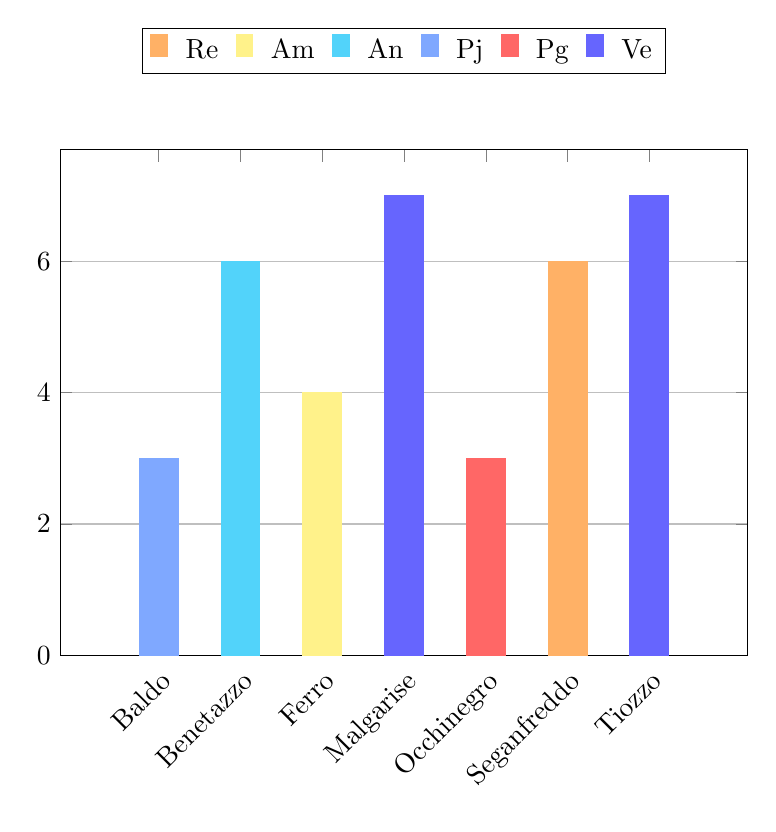
\begin{tikzpicture}
        \begin{axis}[
            width  = 0.85*\textwidth,
            height = 8cm,
            ybar stacked,
            bar width=14pt,
            ymajorgrids = true,
            symbolic x coords={Baldo, Benetazzo, Ferro, Malgarise, Occhinegro, Seganfreddo, Tiozzo},
            xtick = data,
            scaled y ticks = false,
            enlarge x limits=0.2,
            ymin=0,
            legend cell align=left,
            legend style={
                at={(0.5,1.15)},
                anchor=south,
                column sep=1ex,
                legend columns=-1
            },
            xticklabel style={rotate=45, anchor=north east, yshift=0ex, xshift=0ex},
            ]
            \addplot+[ybar, resp, fill=resp, mark=none] plot coordinates {
                (Baldo, 0)
                (Benetazzo, 0)
                (Ferro, 0)
                (Malgarise, 0)
                (Occhinegro, 0)
                (Seganfreddo, 6)
                (Tiozzo, 0)
            };
            \addplot+[ybar, amm, fill=amm, mark=none] plot coordinates {
                (Baldo, 0)
                (Benetazzo, 0)
                (Ferro, 4)
                (Malgarise, 0)
                (Occhinegro, 0)
                (Seganfreddo, 0)
                (Tiozzo, 0)
            };
            \addplot+[ybar, an, fill=an, mark=none] plot coordinates {
                (Baldo, 0)
                (Benetazzo, 6)
                (Ferro, 0)
                (Malgarise, 0)
                (Occhinegro, 0)
                (Seganfreddo, 0)
                (Tiozzo, 0)
            };
            \addplot+[ybar, pj, fill=pj, mark=none] plot coordinates {
                (Baldo, 3)
                (Benetazzo, 0)
                (Ferro, 0)
                (Malgarise, 0)
                (Occhinegro, 0)
                (Seganfreddo, 0)
                (Tiozzo, 0)
            };
            \addplot+[ybar, pg, fill=pg, mark=none] plot coordinates {
                (Baldo, 0)
                (Benetazzo, 0)
                (Ferro, 0)
                (Malgarise, 0)
                (Occhinegro, 3)
                (Seganfreddo, 0)
                (Tiozzo, 0)
            };
            \addplot+[ybar, ver, fill=ver, mark=none] plot coordinates {
                (Baldo, 0)
                (Benetazzo, 0)
                (Ferro, 0)
                (Malgarise, 7)
                (Occhinegro, 0)
                (Seganfreddo, 0)
                (Tiozzo, 7)
            };
            \legend{Re, Am, An, Pj, Pg, Ve}
        \end{axis}
    \end{tikzpicture}
    \caption{Impegno preventivo per ruolo dei membri del team durante il quinto \href{https://7last.github.io/docs/pb/documentazione-interna/glossario\#sprint}{sprint\textsubscript{G}}}
\end{figure}

%---------1_GRAFICO A TORTA-----------%
\begin{figure}[!h]
    \centering
    \begin{tikzpicture}
        \def\printonlypositive#1{\ifdim#1pt>0pt
        #1
        \fi}
        \pie[pos={8,0},radius=3.5,text=legend,
        before number=\printonlypositive,color={resp,amm,an,pj,pg,ver}] { 
             16.7/\href{https://7last.github.io/docs/pb/documentazione-interna/glossario\#responsabile}{Responsabile\textsubscript{G}},
             11.1/\href{https://7last.github.io/docs/pb/documentazione-interna/glossario\#amministratore}{Amministratore\textsubscript{G}},
             16.7/\href{https://7last.github.io/docs/pb/documentazione-interna/glossario\#analista}{Analista\textsubscript{G}},
             8.3/\href{https://7last.github.io/docs/pb/documentazione-interna/glossario\#progettista}{Progettista\textsubscript{G}},
             8.3/\href{https://7last.github.io/docs/pb/documentazione-interna/glossario\#programmatore}{Programmatore\textsubscript{G}},
             38.9/\href{https://7last.github.io/docs/pb/documentazione-interna/glossario\#verificatore}{Verificatore\textsubscript{G}}
        }
        \end{tikzpicture}
    \caption{Ripartizione in percentuale dei ruoli nel quinto \href{https://7last.github.io/docs/pb/documentazione-interna/glossario\#sprint}{sprint\textsubscript{G}}}
\end{figure}


 \newpage
 \subsubsubsection{Consuntivo}

 \subsubsubsubsection{Prospetto orario}
 \begin{table}[!h]
     \centering
     \begin{tabular}{ | l | c | c | c | c | c | c | c | }
         \hline
         \textbf{} & \textbf{Re} & \textbf{Am} &\textbf{An} & \textbf{Pj} & \textbf{Pg} & \textbf{Ve} & \textbf{Totale per persona} \\
         \hline
         Baldo            &  -   &  -   &  -   &  2   &  -   &  -   &  2   \\
         Benetazzo        &  -   &  -   &  8   &  -   &  -   &  -   &  8   \\
         Ferro            &  -   &  7   &  -   &  -   &  -   &  -   &  7   \\
         Malgarise        &  -   &  -   &  -   &  -   &  -   &  5   &  5   \\
         Occhinegro       &  -   &  -   &  -   &  -   &  5   &  -   &  5   \\
         Seganfreddo      &  4   &  -   &  -   &  -   &  -   &  -   &  4   \\
         Tiozzo           &  -   &  -   &  -   &  -   &  -   &  7   &  7   \\
         \hline
         Totale per ruolo &  4   &  7   &  8   &  2   &  5   &  12   &  -   \\
         \hline
     \end{tabular}
     \caption{Consuntivo orario per ruolo dei membri del team durante il quinto \href{https://7last.github.io/docs/pb/documentazione-interna/glossario\#sprint}{sprint\textsubscript{G}}}
 \end{table}

 \subsubsubsubsection{Prospetto economico}
 \begin{table}[!h]
     \centering
     \begin{tabular}{ | l | c | c | c | c | c | }
         \hline
         \textbf{Ruolo} & \textbf{Ore} & \textbf{Costo} & \textbf{Ore rimanenti preventivo} & \textbf{Ore rimanenti consuntivo} \\
         \hline
         \href{https://7last.github.io/docs/pb/documentazione-interna/glossario\#responsabile}{Responsabile\textsubscript{G}}               &  4   &    120,00 € &   31   &   33   \\
         \href{https://7last.github.io/docs/pb/documentazione-interna/glossario\#amministratore}{Amministratore\textsubscript{G}}             &  7   &    140,00 € &   31   &   28   \\
         \href{https://7last.github.io/docs/pb/documentazione-interna/glossario\#analista}{Analista\textsubscript{G}}                   &  8   &    200,00 € &   39   &   37   \\
         \href{https://7last.github.io/docs/pb/documentazione-interna/glossario\#progettista}{Progettista\textsubscript{G}}                &  2   &    50,00 € &   94   &   95   \\
         \href{https://7last.github.io/docs/pb/documentazione-interna/glossario\#programmatore}{Programmatore\textsubscript{G}}              &  5   &    75,00 € &   110   &   108   \\
         \href{https://7last.github.io/docs/pb/documentazione-interna/glossario\#verificatore}{Verificatore\textsubscript{G}}               &  12   &    180,00 € &   133,5   &   135,5   \\
         \hline
         \textbf{Totale preventivo} &  36   &    740,00 € &   438,5   &   -   \\
         \hline
         \textbf{Totale consuntivo} &  38   &    765,00 € &   -   &   436,5   \\
         \hline
     \end{tabular}
     \caption{Consuntivo economico durante il quinto \href{https://7last.github.io/docs/pb/documentazione-interna/glossario\#sprint}{sprint\textsubscript{G}}}
 \end{table}
\newpage
 \subsubsubsubsection{Rischi effettivamente occorsi e loro mitigazione}
 \begin{table}[!h]
     \centering
     \begin{tabular}{ | p{6cm} | p{2.5cm} | p{7.5cm} | }
         \hline
         \textbf{Tipologia} & \textbf{Rischio preventivato} & \textbf{Mitigazione}  \\
         \hline
         Impegni personali o universitari (Rischio \textbf{RO-2})& SI & Comunicato in anticipo gli impegni, lavoro affidato svolto prima o dopo l'impegno.\\
         \hline
     \end{tabular}
     \caption{Rischi effettivamente occorsi e loro mitigazione durante il quinto \href{https://7last.github.io/docs/pb/documentazione-interna/glossario\#sprint}{sprint\textsubscript{G}}}

 \end{table}

 \subsubsubsection{Retrospettiva}
In questo \href{https://7last.github.io/docs/pb/documentazione-interna/glossario\#sprint}{sprint\textsubscript{G}} il gruppo si è concentrato sulla preparazione della documentazione necessaria per la revisione
di avanzamento.
Nonostante alcuni membri abbiano avuto impegni personali e universitari, \textit{7Last} è riuscito a portare a termine
tutte le attività previste, grazie a una comunicazione anticipata degli impegni.\\



\newpage
\subsubsection{Sesto sprint}
\begin{itemize}
	\item Inizio: 2024-05-30
	\item Fine: 2024-06-05
	\item Fine attuale: 2024-06-04
	\item Giorni di ritardo: nessuno
\end{itemize}

\subsubsubsection{Pianificazione}
Dopo aver sostenuto la prima parte della revisione di avanzamento il gruppo si impegnerà a studiare le tecnologie, i business case e i \href{https://7last.github.io/docs/pb/documentazione-interna/glossario\#design-pattern}{design pattern\textsubscript{G}} che verranno impiegati in futuro.
Inoltre continuerà la stesura della documentazione, in particolare:
\begin{itemize}
	\item \href{https://7last.github.io/docs/pb/documentazione-interna/glossario\#piano-di-progetto}{\textit{Piano di Progetto}\textsubscript{G}};
	\item \href{https://7last.github.io/docs/pb/documentazione-interna/glossario\#piano-di-qualifica}{\textit{Piano di Qualifica}\textsubscript{G}};
	\item verbali.
\end{itemize}

\subsubsubsubsection{Rischi attesi}
I rischi attesi per questo periodo sono:
\begin{itemize}
	\item impegni personali o universitari (RO-2).
\end{itemize}
Visto che si avvicina la sessione estiva, alcuni membri del gruppo potrebbero avere impegni personali e universitari che
potrebbero rallentare il lavoro.
Inoltre, il gruppo potrebbe avere dei disaccordi riguardo le scelte da prendere per la  presentazione da preparare in
vista della revisione di avanzamento.

\newpage
\subsubsubsection{Preventivo}
Ruoli coinvolti: \href{https://7last.github.io/docs/pb/documentazione-interna/glossario\#responsabile}{Responsabile\textsubscript{G}} (Re), \href{https://7last.github.io/docs/pb/documentazione-interna/glossario\#amministratore}{Amministratore\textsubscript{G}} (Am), \href{https://7last.github.io/docs/pb/documentazione-interna/glossario\#analista}{Analista\textsubscript{G}} (An), \href{https://7last.github.io/docs/pb/documentazione-interna/glossario\#progettista}{Progettista\textsubscript{G}} (Pj), \href{https://7last.github.io/docs/pb/documentazione-interna/glossario\#programmatore}{Programmatore\textsubscript{G}} (Pg), \href{https://7last.github.io/docs/pb/documentazione-interna/glossario\#verificatore}{Verificatore\textsubscript{G}} (Ve).
\begin{table}[!h]
	\centering
	\begin{tabular}{ | l | c | c | c | c | c | c | c | }
		\hline
		\textbf{} & \textbf{Re} & \textbf{Am} &\textbf{An} & \textbf{Pj} & \textbf{Pg} & \textbf{Ve} & \textbf{Totale per persona} \\
		\hline
		Baldo            &  -   &  -   &  6   &  -   &  -   &  -   &  6   \\
		Benetazzo        &  -   &  -   &  -   &  6   &  -   &  -   &  6   \\
		Ferro            &  4   &  -   &  -   &  -   &  -   &  -   &  4   \\
		Malgarise        &  -   &  -   &  -   &  -   &  -   &  5   &  5   \\
		Occhinegro       &  -   &  5   &  -   &  -   &  -   &  -   &  5   \\
		Seganfreddo      &  -   &  -   &  -   &  6   &  -   &  5   &  11   \\
		Tiozzo           &  -   &  -   &  6   &  -   &  -   &  -   &  6   \\
		\hline
		Totale per ruolo &  4   &  5   &  12   &  12   &  0   &  10   &  -   \\
		\hline
	\end{tabular}
	\caption{Preventivo orario per ruolo dei membri del team durante il sesto \href{https://7last.github.io/docs/pb/documentazione-interna/glossario\#sprint}{sprint\textsubscript{G}}}

\end{table}

\newpage
%---------1_ISTOGRAMMA-----------%
\begin{figure}[!h]
	\centering
	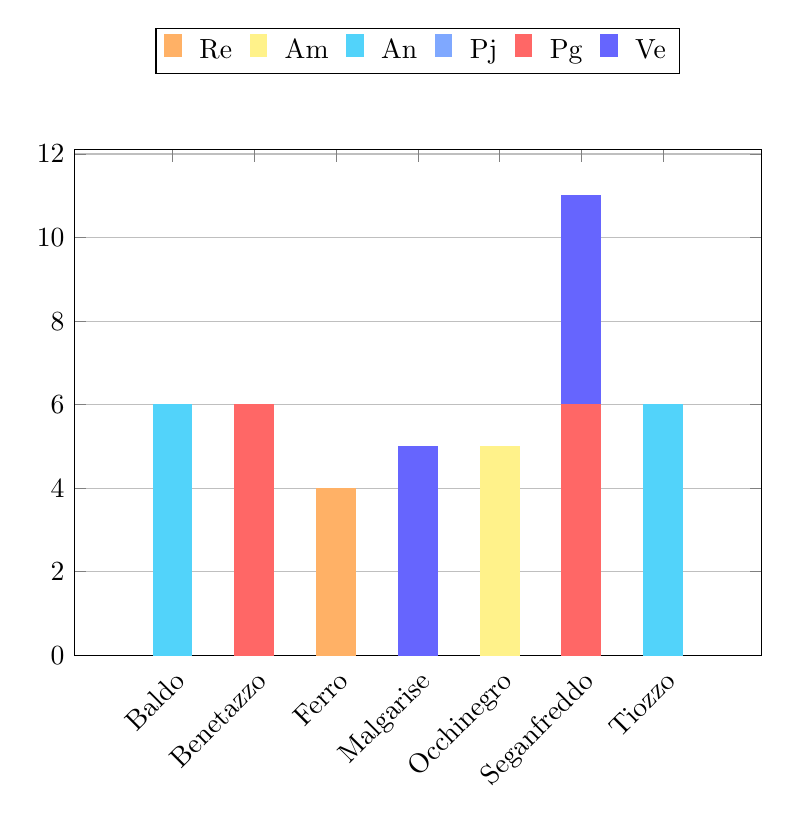
\begin{tikzpicture}
		\begin{axis}[
			width  = 0.85*\textwidth,
			height = 8cm,
			ybar stacked,
			bar width=14pt,
			ymajorgrids = true,
			symbolic x coords={Baldo, Benetazzo, Ferro, Malgarise, Occhinegro, Seganfreddo, Tiozzo},
			xtick = data,
			scaled y ticks = false,
			enlarge x limits=0.2,
			ymin=0,
			legend cell align=left,
			legend style={
				at={(0.5,1.15)},
				anchor=south,
				column sep=1ex,
				legend columns=-1
			},
			xticklabel style={rotate=45, anchor=north east, yshift=0ex, xshift=0ex},
		]
			\addplot+[ybar, resp, fill=resp, mark=none] plot coordinates {
				(Baldo, 0)
				(Benetazzo, 0)
				(Ferro, 4)
				(Malgarise, 0)
				(Occhinegro, 0)
				(Seganfreddo, 0)
				(Tiozzo, 0)
			};
			\addplot+[ybar, amm, fill=amm, mark=none] plot coordinates {
				(Baldo, 0)
				(Benetazzo, 0)
				(Ferro, 0)
				(Malgarise, 0)
				(Occhinegro, 5)
				(Seganfreddo, 0)
				(Tiozzo, 0)
			};
			\addplot+[ybar, an, fill=an, mark=none] plot coordinates {
				(Baldo, 6)
				(Benetazzo, 0)
				(Ferro, 0)
				(Malgarise, 0)
				(Occhinegro, 0)
				(Seganfreddo, 0)
				(Tiozzo, 6)
			};
			\addplot+[ybar, pj, fill=pj, mark=none] plot coordinates {
				(Baldo, 0)
				(Benetazzo, 0)
				(Ferro, 0)
				(Malgarise, 0)
				(Occhinegro, 0)
				(Seganfreddo, 0)
				(Tiozzo, 0)
			};
			\addplot+[ybar, pg, fill=pg, mark=none] plot coordinates {
				(Baldo, 0)
				(Benetazzo, 6)
				(Ferro, 0)
				(Malgarise, 0)
				(Occhinegro, 0)
				(Seganfreddo, 6)
				(Tiozzo, 0)
			};
			\addplot+[ybar, ver, fill=ver, mark=none] plot coordinates {
				(Baldo, 0)
				(Benetazzo, 0)
				(Ferro, 0)
				(Malgarise, 5)
				(Occhinegro, 0)
				(Seganfreddo, 5)
				(Tiozzo, 0)
			};
			\legend{Re, Am, An, Pj, Pg, Ve}
		\end{axis}
	\end{tikzpicture}
	\caption{Impegno preventivo per ruolo dei membri del team durante il sesto \href{https://7last.github.io/docs/pb/documentazione-interna/glossario\#sprint}{sprint\textsubscript{G}}}

\end{figure}

%---------1_GRAFICO A TORTA-----------%
\begin{figure}[!h]
	\centering
	\begin{tikzpicture}
		\def\printonlypositive#1{\ifdim#1pt>0pt#1\%\else\fi}
		\pie[pos={8,0},radius=3.5,text=legend,
			before number=\printonlypositive, after number=, color={resp,amm,an,pj,pg,ver}] {
			9.3/\href{https://7last.github.io/docs/pb/documentazione-interna/glossario\#responsabile}{Responsabile\textsubscript{G}},
			11.6/\href{https://7last.github.io/docs/pb/documentazione-interna/glossario\#amministratore}{Amministratore\textsubscript{G}},
			27.9/\href{https://7last.github.io/docs/pb/documentazione-interna/glossario\#analista}{Analista\textsubscript{G}},
			27.9/\href{https://7last.github.io/docs/pb/documentazione-interna/glossario\#progettista}{Progettista\textsubscript{G}},
			0.0/\href{https://7last.github.io/docs/pb/documentazione-interna/glossario\#programmatore}{Programmatore\textsubscript{G}},
			23.3/\href{https://7last.github.io/docs/pb/documentazione-interna/glossario\#verificatore}{Verificatore\textsubscript{G}}
		}
	\end{tikzpicture}
	\caption{Ripartizione in percentuale dei ruoli nel sesto \href{https://7last.github.io/docs/pb/documentazione-interna/glossario\#sprint}{sprint\textsubscript{G}}}

\end{figure}
\newpage
\subsubsubsection{Consuntivo}
 Tutte le attività e le scadenze preventivate per questo \href{https://7last.github.io/docs/pb/documentazione-interna/glossario\#sprint}{sprint\textsubscript{G}} sono state rispettate.

\subsubsubsubsection{Prospetto orario} 
\begin{table}[!h]
    \centering
    \begin{tabular}{ | l | c | c | c | c | c | c | c | }
        \hline
        \textbf{} & \textbf{Re} & \textbf{Am} &\textbf{An} & \textbf{Pj} & \textbf{Pg} & \textbf{Ve} & \textbf{Totale per persona} \\
        \hline
        Baldo            &  -   &  -   &  5   &  -   &  -   &  -   &  5   \\
        Benetazzo        &  -   &  -   &  -   &  6   &  -   &  -   &  6   \\
        Ferro            &  5   &  -   &  -   &  -   &  -   &  -   &  5   \\
        Malgarise        &  -   &  -   &  -   &  -   &  -   &  6   &  6   \\
        Occhinegro       &  -   &  5   &  -   &  -   &  -   &  -   &  5   \\
        Seganfreddo      &  -   &  -   &  -   &  5   &  -   &  4   &  9   \\
        Tiozzo           &  -   &  -   &  7   &  -   &  -   &  -   &  7   \\
        \hline
        Totale per ruolo &  5   &  5   &  12   &  11   &  -   &  10   &  -   \\
        \hline
    \end{tabular}
    \caption{Consuntivo orario per ruolo dei membri del team durante il sesto \href{https://7last.github.io/docs/pb/documentazione-interna/glossario\#sprint}{sprint\textsubscript{G}}} 
\end{table}

\subsubsubsubsection{Prospetto economico}
\begin{table}[!h]
    \centering
    \begin{tabular}{ | l | c | c | c | c | c | }
        \hline
        \textbf{Ruolo} & \textbf{Ore} & \textbf{Costo} & \textbf{Ore rimanenti preventivo} & \textbf{Ore rimanenti consuntivo} \\
        \hline
        \href{https://7last.github.io/docs/pb/documentazione-interna/glossario\#responsabile}{Responsabile\textsubscript{G}}			&  5   &    150,00 € &   29   &   28   \\
        \href{https://7last.github.io/docs/pb/documentazione-interna/glossario\#amministratore}{Amministratore\textsubscript{G}}		&  5   &    100,00 € &   23   &   23   \\
        \href{https://7last.github.io/docs/pb/documentazione-interna/glossario\#analista}{Analista\textsubscript{G}}                   &  12   &    300,00 € &   25   &   25   \\
        \href{https://7last.github.io/docs/pb/documentazione-interna/glossario\#progettista}{Progettista\textsubscript{G}}                										  &  11   &    275,00 € &   83   &   84   \\
        \href{https://7last.github.io/docs/pb/documentazione-interna/glossario\#programmatore}{Programmatore\textsubscript{G}}              										  &  0   &    0,00 € &   108   &   108   \\
        \href{https://7last.github.io/docs/pb/documentazione-interna/glossario\#verificatore}{Verificatore\textsubscript{G}}               &  10   &    150,00 € &   125,5   &   125,5   \\
        \hline
        \textbf{Totale preventivo} &  43   &    970,00 € &   393,5   &   -   \\
        \hline
        \textbf{Totale consuntivo} &  43   &    975,00 € &   -   &   393,5   \\
        \hline
    \end{tabular}
    \caption{Consuntivo economico durante il sesto \href{https://7last.github.io/docs/pb/documentazione-interna/glossario\#sprint}{sprint\textsubscript{G}}}

\end{table}
\newpage
\subsubsubsubsection{Rischi effettivamente occorsi e loro mitigazione}
\begin{table}[!h]
    \centering
    \begin{tabular}{ | p{6cm} | p{2.5cm} | p{7.5cm} | }
        \hline
        \textbf{Tipologia} & \textbf{Rischio preventivato} & \textbf{Mitigazione}  \\
        \hline
        Impegni personali o universitari (Rischio \textbf{RO-2})& SI & Comunicato in anticipo gli impegni, lavoro affidato svolto prima o dopo l’impegno. \\
        \hline
    \end{tabular}
    \caption{Rischi effettivamente occorsi e loro mitigazione durante il sesto \href{https://7last.github.io/docs/pb/documentazione-interna/glossario\#sprint}{sprint\textsubscript{G}}}
\end{table}

\subsubsubsection{Retrospettiva}
Durante lo \href{https://7last.github.io/docs/pb/documentazione-interna/glossario\#sprint}{sprint\textsubscript{G}} corrente il gruppo ha sostenuto la prima metà della revisione di avanzamento. Nonostante gli impegni personali dovuti alla sessione estiva, il gruppo è riuscito a portare a termine tutte le attività previste con un giorno di anticipo.



\newpage
\subsection{Product Baseline}
\subsubsection{Settimo sprint}
\begin{itemize}
	\item Inizio: 2024-06-06
	\item Fine: 2024-06-12
	\item Fine attuale: 2024-06-12
	\item Giorni di ritardo: nessuno
\end{itemize}

\subsubsubsection{Pianificazione}
In vista della seconda parte della revisione \href{https://7last.github.io/docs/pb/documentazione-interna/glossario\#requirements-and-technology-baseline}{RTB\textsubscript{G}} il gruppo si impegnerà prevalentemente nella preparazione della presentazione e procederò con l'avanzamento del progetto. In particolare verranno aggiunte nuove tipologie di sensori, studiate le metodologie di testing e verrà iniziata l'analisi delle possibili architetture. In secondo luogo continuerà la stesura della documentazione, ovvero:
\begin{itemize}
	\item \href{https://7last.github.io/docs/pb/documentazione-interna/glossario\#piano-di-progetto}{\textit{Piano di Progetto}\textsubscript{G}};
	\item \href{https://7last.github.io/docs/pb/documentazione-interna/glossario\#piano-di-qualifica}{\textit{Piano di Qualifica}\textsubscript{G}};
	\item \href{https://7last.github.io/docs/pb/documentazione-interna/glossario\#glossario}{\textit{Glossario}\textsubscript{G}};
	\item verbali.
\end{itemize}

\subsubsubsubsection{Rischi attesi}
I rischi attesi per questo periodo sono:
\begin{itemize}
	\item impegni personali o universitari (RO-2);
	\item ritardi rispetto alle tempistiche previste (RO-3);
	\item disaccordi all'interno del gruppo (RC-1).
\end{itemize}
A causa della sessione estiva, alcuni membri del gruppo potrebbero avere impegni personali e universitari in grado di impattare sull'avanzamento del lavoro. In aggiunta il gruppo potrebbe avere dei disaccordi riguardo le scelte da prendere per la presentazione da preparare in vista della seconda parte della revisione di avanzamento \href{https://7last.github.io/docs/pb/documentazione-interna/glossario\#requirements-and-technology-baseline}{RTB\textsubscript{G}}. Tutto questo potrebbe portare a ritardi rispetto alle tempistiche previste e a un clima di lavoro non ottimale.

\newpage
\subsubsubsection{Preventivo}
Ruoli coinvolti: \href{https://7last.github.io/docs/pb/documentazione-interna/glossario\#responsabile}{Responsabile\textsubscript{G}} (Re), \href{https://7last.github.io/docs/pb/documentazione-interna/glossario\#amministratore}{Amministratore\textsubscript{G}} (Am), \href{https://7last.github.io/docs/pb/documentazione-interna/glossario\#analista}{Analista\textsubscript{G}} (An), \href{https://7last.github.io/docs/pb/documentazione-interna/glossario\#progettista}{Progettista\textsubscript{G}} (Pj), \href{https://7last.github.io/docs/pb/documentazione-interna/glossario\#programmatore}{Programmatore\textsubscript{G}} (Pg), \href{https://7last.github.io/docs/pb/documentazione-interna/glossario\#verificatore}{Verificatore\textsubscript{G}} (Ve).
\begin{table}[!h]
	\centering
	\begin{tabular}{ | l | c | c | c | c | c | c | c | }
		\hline
		\textbf{} & \textbf{Re} & \textbf{Am} &\textbf{An} & \textbf{Pj} & \textbf{Pg} & \textbf{Ve} & \textbf{Totale per persona} \\
		\hline
		Baldo            &  4   &  -   &  -   &  -   &  -   &  -   &  4   \\
		Benetazzo        &  -   &  -   &  -   &  -   &  8   &  -   &  8   \\
		Ferro            &  -   &  -   &  -   & 10   &  -   &  -   & 10   \\
		Malgarise        &  -   &  4   &  -   &  -   &  -   &  -   &  4   \\
		Occhinegro       &  -   &  -   & 12   &  -   &  -   &  -   & 12   \\
		Seganfreddo      &  -   &  -   &  -   &  -   &  8   &  -   &  8   \\
		Tiozzo           &  -   &  -   &  -   &  -   &  -   &  8   &  8   \\
		\hline
		Totale per ruolo &  4   &  4   & 12   & 10   & 16   &  8   &  -   \\
		\hline
	\end{tabular}
	\caption{Preventivo orario per ruolo dei membri del team durante il settimo \href{https://7last.github.io/docs/pb/documentazione-interna/glossario\#sprint}{sprint\textsubscript{G}}}

\end{table}

%---------1_ISTOGRAMMA-----------%
\begin{figure}[!h]
	\centering
	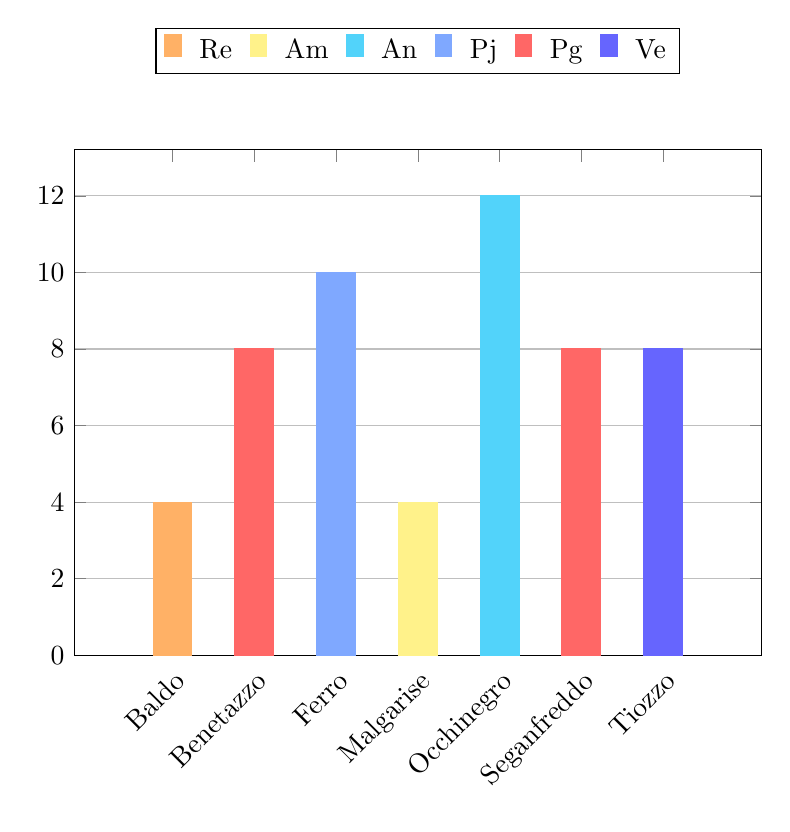
\begin{tikzpicture}
		\begin{axis}[
			width  = 0.85*\textwidth,
			height = 8cm,
			ybar stacked,
			bar width=14pt,
			ymajorgrids = true,
			symbolic x coords={Baldo, Benetazzo, Ferro, Malgarise, Occhinegro, Seganfreddo, Tiozzo},
			xtick = data,
			scaled y ticks = false,
			enlarge x limits=0.2,
			ymin=0,
			legend cell align=left,
			legend style={
				at={(0.5,1.15)},
				anchor=south,
				column sep=1ex,
				legend columns=-1
			},
			xticklabel style={rotate=45, anchor=north east, yshift=0ex, xshift=0ex},
		]
			\addplot+[ybar, resp, fill=resp, mark=none] plot coordinates {
				(Baldo, 4)
				(Benetazzo, 0)
				(Ferro, 0)
				(Malgarise, 0)
				(Occhinegro, 0)
				(Seganfreddo, 0)
				(Tiozzo, 0)
			};
			\addplot+[ybar, amm, fill=amm, mark=none] plot coordinates {
				(Baldo, 0)
				(Benetazzo, 0)
				(Ferro, 0)
				(Malgarise, 4)
				(Occhinegro, 0)
				(Seganfreddo, 0)
				(Tiozzo, 0)
			};
			\addplot+[ybar, an, fill=an, mark=none] plot coordinates {
				(Baldo, 0)
				(Benetazzo, 0)
				(Ferro, 0)
				(Malgarise, 0)
				(Occhinegro, 12)
				(Seganfreddo, 0)
				(Tiozzo, 0)
			};
			\addplot+[ybar, pj, fill=pj, mark=none] plot coordinates {
				(Baldo, 0)
				(Benetazzo, 0)
				(Ferro, 10)
				(Malgarise, 0)
				(Occhinegro, 0)
				(Seganfreddo, 0)
				(Tiozzo, 0)
			};
			\addplot+[ybar, pg, fill=pg, mark=none] plot coordinates {
				(Baldo, 0)
				(Benetazzo, 8)
				(Ferro, 0)
				(Malgarise, 0)
				(Occhinegro, 0)
				(Seganfreddo, 8)
				(Tiozzo, 0)
			};
			\addplot+[ybar, ver, fill=ver, mark=none] plot coordinates {
				(Baldo, 0)
				(Benetazzo, 0)
				(Ferro, 0)
				(Malgarise, 0)
				(Occhinegro, 0)
				(Seganfreddo, 0)
				(Tiozzo, 8)
			};
			\legend{Re, Am, An, Pj, Pg, Ve}
		\end{axis}
	\end{tikzpicture}
	\caption{Impegno preventivo per ruolo dei membri del team durante il settimo \href{https://7last.github.io/docs/pb/documentazione-interna/glossario\#sprint}{sprint\textsubscript{G}}}

\end{figure}

%---------1_GRAFICO A TORTA-----------%
\begin{figure}[!h]
	\centering
	\begin{tikzpicture}
		\def\printonlypositive#1{\ifdim#1pt>0pt#1\%\else\fi}
		\pie[pos={8,0},radius=3.5,text=legend,
			before number=\printonlypositive, after number=, color={resp,amm,an,pj,pg,ver}] {
			7.4/\href{https://7last.github.io/docs/pb/documentazione-interna/glossario\#responsabile}{Responsabile\textsubscript{G}},
			7.4/\href{https://7last.github.io/docs/pb/documentazione-interna/glossario\#amministratore}{Amministratore\textsubscript{G}},
			22.2/\href{https://7last.github.io/docs/pb/documentazione-interna/glossario\#analista}{Analista\textsubscript{G}},
			18.5/\href{https://7last.github.io/docs/pb/documentazione-interna/glossario\#progettista}{Progettista\textsubscript{G}},
			29.6/\href{https://7last.github.io/docs/pb/documentazione-interna/glossario\#programmatore}{Programmatore\textsubscript{G}},
			14.8/\href{https://7last.github.io/docs/pb/documentazione-interna/glossario\#verificatore}{Verificatore\textsubscript{G}}
		}
	\end{tikzpicture}
	\caption{Ripartizione in percentuale dei ruoli nel settimo \href{https://7last.github.io/docs/pb/documentazione-interna/glossario\#sprint}{sprint\textsubscript{G}}}

\end{figure}
\newpage
\subsubsubsection{Consuntivo}
 A seguito del colloquio con il professor Vardanega è stata prestata una maggiore attenzione nello studio dei test e dell'architettura da implementare. Le scadenze sono state rispettate. Rispetto a quanto preventivato le attività pianificate hanno richiesto meno tempo del previsto, abbassando notevolmente i costi previsti per questo \href{https://7last.github.io/docs/pb/documentazione-interna/glossario\#sprint}{sprint\textsubscript{G}}.

\subsubsubsubsection{Prospetto orario} 
\begin{table}[!h]
    \centering
    \begin{tabular}{ | l | c | c | c | c | c | c | c | }
        \hline
        \textbf{} & \textbf{Re} & \textbf{Am} &\textbf{An} & \textbf{Pj} & \textbf{Pg} & \textbf{Ve} & \textbf{Totale per persona} \\
        \hline
        Baldo            &  3   &  -   &  -   &  -   &  -   &  -   &  3   \\
        Benetazzo        &  -   &  -   &  -   &  -   &  7,5 &  -   &  7,5 \\
        Ferro            &  -   &  -   &  -   &  6   &  -   &  -   &  6   \\
        Malgarise        &  -   &  4   &  -   &  -   &  -   &  -   &  4   \\
        Occhinegro       &  -   &  -   &  9   &  -   &  -   &  -   &  9   \\
        Seganfreddo      &  -   &  -   &  -   &  -   &  7   &  -   &  7   \\
        Tiozzo           &  -   &  -   &  -   &  -   &  -   &  6,5 &  6,5 \\
        \hline
        Totale per ruolo &  3   &  4   &  9   &  6   & 14,5 &  6,5  &  -  \\
        \hline
    \end{tabular}
    \caption{Consuntivo orario per ruolo dei membri del team durante il settimo \href{https://7last.github.io/docs/pb/documentazione-interna/glossario\#sprint}{sprint\textsubscript{G}}}
\end{table}

\subsubsubsubsection{Prospetto economico} 
\begin{table}[!h]
    \centering
    \begin{tabular}{ | l | c | c | c | c | c | }
        \hline
        \textbf{Ruolo} & \textbf{Ore} & \textbf{Costo} & \textbf{Ore rimanenti preventivo} & \textbf{Ore rimanenti consuntivo} \\
        \hline
        \href{https://7last.github.io/docs/pb/documentazione-interna/glossario\#responsabile}{Responsabile\textsubscript{G}}           &  3    &     90,00 € &  24   &  25   \\
        \href{https://7last.github.io/docs/pb/documentazione-interna/glossario\#amministratore}{Amministratore\textsubscript{G}}       &  4    &     80,00 € &  19   &  19   \\
        \href{https://7last.github.io/docs/pb/documentazione-interna/glossario\#analista}{Analista\textsubscript{G}}                   &  9    &    225,00 € &  13   &  16   \\
        \href{https://7last.github.io/docs/pb/documentazione-interna/glossario\#progettista}{Progettista\textsubscript{G}}             &  6    &    150,00 € &  74   &  78   \\
        \href{https://7last.github.io/docs/pb/documentazione-interna/glossario\#programmatore}{Programmatore\textsubscript{G}}         & 14,5  &    217,50 € &  92   &  93,5 \\
        \href{https://7last.github.io/docs/pb/documentazione-interna/glossario\#verificatore}{Verificatore\textsubscript{G}}           &  6,5  &     97,50 € & 117,5 & 119   \\
        \hline
        \textbf{Totale preventivo} &  54   &    1110,00 € &   339,5   &   -   \\
        \hline
        \textbf{Totale consuntivo} &  43   &     860,00 € &   -   &   350,5   \\
        \hline
    \end{tabular}
    \caption{Consuntivo economico durante il settimo \href{https://7last.github.io/docs/pb/documentazione-interna/glossario\#sprint}{sprint\textsubscript{G}}}

\end{table}

\subsubsubsubsection{Rischi effettivamente occorsi e loro mitigazione}
\begin{table}[!h]
    \centering
    \begin{tabular}{ | p{6cm} | p{2.5cm} | p{7.5cm} | }
        \hline
        \textbf{Tipologia} & \textbf{Rischio preventivato} & \textbf{Mitigazione}  \\
        \hline
        Impegni personali o universitari (Rischio \textbf{RO-2})& SI & Comunicato in anticipo gli impegni, lavoro affidato svolto prima o dopo l’impegno. \\
        \hline
    \end{tabular}
    \caption{Rischi effettivamente occorsi e loro mitigazione durante il settimo \href{https://7last.github.io/docs/pb/documentazione-interna/glossario\#sprint}{sprint\textsubscript{G}}}
\end{table}

\subsubsubsection{Retrospettiva}
Durante lo \href{https://7last.github.io/docs/pb/documentazione-interna/glossario\#sprint}{sprint\textsubscript{G}} corrente il gruppo ha sostenuto la seconda metà della revisione di avanzamento. Questo periodo è stato adattato per aggiungere dei task consigliati dal professore e nonostante gli impegni personali dovuti alla sessione estiva, il gruppo è riuscito a portare a termine tutte le attività previste.


\newpage
\subsubsection{Ottavo sprint}
\begin{itemize}
	\item Inizio: 2024-06-13
	\item Fine: 2024-06-19
	\item Fine attuale: 2024-06-19
	\item Giorni di ritardo: nessuno
\end{itemize}

\subsubsubsection{Pianificazione}
Procederemo con lo sviluppo dei sensori di diverse tipologie (precipitazioni, umidità, colonnine di ricarica, livello dei fiumi), effettueremo dei miglioramenti sul sito di presentazione della documentazione come suggerito dal professor Vardanega nella valutazione \href{https://7last.github.io/docs/pb/documentazione-interna/glossario\#requirements-and-technology-baseline}{RTB\textsubscript{G}}. Proseguiremo con l'aggiornamento della consueta documentazione (\href{https://7last.github.io/docs/pb/documentazione-interna/glossario\#piano-di-progetto}{PdP\textsubscript{G}}, \href{https://7last.github.io/docs/pb/documentazione-interna/glossario\#piano-di-qualifica}{PdQ\textsubscript{G}}, \href{https://7last.github.io/docs/pb/documentazione-interna/glossario\#glossario}{Glo\textsubscript{G}}, verbali), oltre a cominciare la stesura dei documenti \textit{Specifica Tecnica} e \textit{Manuale Utente}.

\subsubsubsubsection{Rischi attesi}
I rischi attesi per questo periodo sono:
\begin{itemize}
	\item impegni personali o universitari (RO-2);
	\item ritardi rispetto alle tempistiche previste (RO-3).
\end{itemize}
Rimangono i rischi già preventivati in precedenza legati agli impegni universitari, in quanto la sessione estiva è ancora in corso. Sempre per lo stesso motivo, il gruppo potrebbe avere dei ritardi rispetto alle tempistiche previste.

\newpage
\subsubsubsection{Preventivo}
Ruoli coinvolti: \href{https://7last.github.io/docs/pb/documentazione-interna/glossario\#responsabile}{Responsabile\textsubscript{G}} (Re), \href{https://7last.github.io/docs/pb/documentazione-interna/glossario\#amministratore}{Amministratore\textsubscript{G}} (Am), \href{https://7last.github.io/docs/pb/documentazione-interna/glossario\#analista}{Analista\textsubscript{G}} (An), \href{https://7last.github.io/docs/pb/documentazione-interna/glossario\#progettista}{Progettista\textsubscript{G}} (Pj), \href{https://7last.github.io/docs/pb/documentazione-interna/glossario\#programmatore}{Programmatore\textsubscript{G}} (Pg), \href{https://7last.github.io/docs/pb/documentazione-interna/glossario\#verificatore}{Verificatore\textsubscript{G}} (Ve).
\begin{table}[!h]
	\centering
	\begin{tabular}{ | l | c | c | c | c | c | c | c | }
		\hline
		\textbf{} & \textbf{Re} & \textbf{Am} &\textbf{An} & \textbf{Pj} & \textbf{Pg} & \textbf{Ve} & \textbf{Totale per persona} \\
		\hline			    %RE    %AM    %AN    %PJ   %PG     %VE   %TOT
		Baldo            &  -   &  -   &  -   &  -   & 12   &  -   & 12   \\
		Benetazzo        &  -   &  4   &  -   &  -   &  -   &  -   &  4   \\
		Ferro            &  -   &  -   &  -   &  -   &  -   & 12   & 12   \\
		Malgarise        &  4   &  -   &  -   &  -   &  -   &  -   &  4   \\
		Occhinegro       &  -   &  -   &  -   &  8   &  -   &  -   &  8   \\
		Seganfreddo      &  -   &  -   &  8   &  -   &  -   &  -   &  8   \\
		Tiozzo           &  -   &  -   &  -   &  8   &  -   &  -   &  8   \\
		\hline
		Totale per ruolo &  4   &  4   &  8   & 16   & 12   & 12   &  -   \\
		\hline
	\end{tabular}
	\caption{Preventivo orario per ruolo dei membri del team durante l'ottavo \href{https://7last.github.io/docs/pb/documentazione-interna/glossario\#sprint}{sprint\textsubscript{G}}}

\end{table}

%---------1_ISTOGRAMMA-----------%
\begin{figure}[!h]
	\centering
	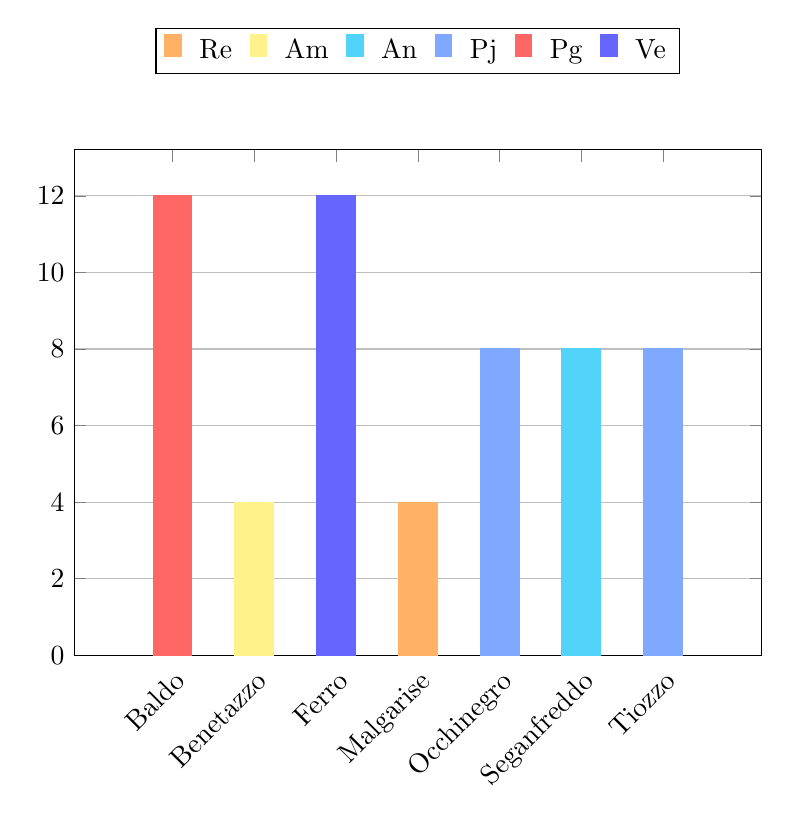
\begin{tikzpicture}
		\begin{axis}[
			width  = 0.85*\textwidth,
			height = 8cm,
			ybar stacked,
			bar width=14pt,
			ymajorgrids = true,
			symbolic x coords={Baldo, Benetazzo, Ferro, Malgarise, Occhinegro, Seganfreddo, Tiozzo},
			xtick = data,
			scaled y ticks = false,
			enlarge x limits=0.2,
			ymin=0,
			legend cell align=left,
			legend style={
				at={(0.5,1.15)},
				anchor=south,
				column sep=1ex,
				legend columns=-1
			},
			xticklabel style={rotate=45, anchor=north east, yshift=0ex, xshift=0ex},
		]
			\addplot+[ybar, resp, fill=resp, mark=none] plot coordinates {
				(Baldo, 0)
				(Benetazzo, 0)
				(Ferro, 0)
				(Malgarise, 4)
				(Occhinegro, 0)
				(Seganfreddo, 0)
				(Tiozzo, 0)
			};
			\addplot+[ybar, amm, fill=amm, mark=none] plot coordinates {
				(Baldo, 0)
				(Benetazzo, 4)
				(Ferro, 0)
				(Malgarise, 0)
				(Occhinegro, 0)
				(Seganfreddo, 0)
				(Tiozzo, 0)
			};
			\addplot+[ybar, an, fill=an, mark=none] plot coordinates {
				(Baldo, 0)
				(Benetazzo, 0)
				(Ferro, 0)
				(Malgarise, 0)
				(Occhinegro, 0)
				(Seganfreddo, 8)
				(Tiozzo, 0)
			};
			\addplot+[ybar, pj, fill=pj, mark=none] plot coordinates {
				(Baldo, 0)
				(Benetazzo, 0)
				(Ferro, 0)
				(Malgarise, 0)
				(Occhinegro, 8)
				(Seganfreddo, 0)
				(Tiozzo, 8)
			};
			\addplot+[ybar, pg, fill=pg, mark=none] plot coordinates {
				(Baldo, 12)
				(Benetazzo, 0)
				(Ferro, 0)
				(Malgarise, 0)
				(Occhinegro, 0)
				(Seganfreddo, 0)
				(Tiozzo, 0)
			};
			\addplot+[ybar, ver, fill=ver, mark=none] plot coordinates {
				(Baldo, 0)
				(Benetazzo, 0)
				(Ferro, 12)
				(Malgarise, 0)
				(Occhinegro, 0)
				(Seganfreddo, 0)
				(Tiozzo, 0)
			};
			\legend{Re, Am, An, Pj, Pg, Ve}
		\end{axis}
	\end{tikzpicture}
	\caption{Impegno preventivo per ruolo dei membri del team durante l'ottavo \href{https://7last.github.io/docs/pb/documentazione-interna/glossario\#sprint}{sprint\textsubscript{G}}}

\end{figure}

%---------1_GRAFICO A TORTA-----------%
\begin{figure}[!h]
	\centering
	\begin{tikzpicture}
		\def\printonlypositive#1{\ifdim#1pt>0pt#1\%\else\fi}
		\pie[pos={8,0},radius=3.5,text=legend,
			before number=\printonlypositive, after number=, color={resp,amm,an,pj,pg,ver}] {
			7.1/\href{https://7last.github.io/docs/pb/documentazione-interna/glossario\#responsabile}{Responsabile\textsubscript{G}},
			7.1/\href{https://7last.github.io/docs/pb/documentazione-interna/glossario\#amministratore}{Amministratore\textsubscript{G}},
			14.3/\href{https://7last.github.io/docs/pb/documentazione-interna/glossario\#analista}{Analista\textsubscript{G}},
			28.6/\href{https://7last.github.io/docs/pb/documentazione-interna/glossario\#progettista}{Progettista\textsubscript{G}},
			21.4/\href{https://7last.github.io/docs/pb/documentazione-interna/glossario\#programmatore}{Programmatore\textsubscript{G}},
			21.4/\href{https://7last.github.io/docs/pb/documentazione-interna/glossario\#verificatore}{Verificatore\textsubscript{G}}
		}
	\end{tikzpicture}
	\caption{Ripartizione in percentuale dei ruoli nell'ottavo \href{https://7last.github.io/docs/pb/documentazione-interna/glossario\#sprint}{sprint\textsubscript{G}}}

\end{figure}

\subsubsubsection{Consuntivo}
 Le scadenze sono state rispettate e l'azienda ha approvato i cambiamenti e le aggiunte effettuate. Le ore preventivate si sono rivelate pressoché corrette, siamo riusciti quindi a rispettare la spesa prevista.

\subsubsubsubsection{Prospetto orario} 
\begin{table}[!h]
    \centering
    \begin{tabular}{ | l | c | c | c | c | c | c | c | }
        \hline
        \textbf{} & \textbf{Re} & \textbf{Am} &\textbf{An} & \textbf{Pj} & \textbf{Pg} & \textbf{Ve} & \textbf{Totale per persona} \\
        \hline			    %RE    %AM    %AN    %PJ   %PG     %VE   %TOT
        Baldo            &  -   &  -   &  -   &  -   & 13   &  -   & 13   \\
		Benetazzo        &  -   &  4   &  -   &  -   &  -   &  -   &  4   \\
		Ferro            &  -   &  -   &  -   &  -   &  -   & 12   & 12   \\
		Malgarise        &  4   &  -   &  -   &  -   &  -   &  -   &  4   \\
		Occhinegro       &  -   &  -   &  -   &  8   &  -   &  -   &  8   \\
		Seganfreddo      &  -   &  -   &  7,5 &  -   &  -   &  -   &  7.5 \\
		Tiozzo           &  -   &  -   &  -   &  7   &  -   &  -   &  7   \\
		\hline
		Totale per ruolo &  4   &  4   &  7,5 & 15   & 13   & 12   &  -   \\
        \hline
    \end{tabular}
    \caption{Consuntivo orario per ruolo dei membri del team durante l'ottavo \href{https://7last.github.io/docs/pb/documentazione-interna/glossario\#sprint}{sprint\textsubscript{G}}}
\end{table}

\newpage
\subsubsubsubsection{Prospetto economico} 
\begin{table}[!h]
    \centering
    \begin{tabular}{ | l | c | c | c | c | c | }
        \hline
        \textbf{Ruolo} & \textbf{Ore} & \textbf{Costo} & \textbf{Ore rimanenti preventivo} & \textbf{Ore rimanenti consuntivo} \\
        \hline
        \href{https://7last.github.io/docs/pb/documentazione-interna/glossario\#responsabile}{Responsabile\textsubscript{G}}     &  4   &    120,00 € &  21   &  21   \\
        \href{https://7last.github.io/docs/pb/documentazione-interna/glossario\#amministratore}{Amministratore\textsubscript{G}} &  4   &     80,00 € &  15   &  15   \\
        \href{https://7last.github.io/docs/pb/documentazione-interna/glossario\#analista}{Analista\textsubscript{G}}             &  7,5 &    187,50 € &   8   &   8,5 \\
        \href{https://7last.github.io/docs/pb/documentazione-interna/glossario\#progettista}{Progettista\textsubscript{G}}       & 15   &    375,00 € &  62   &  63   \\
        \href{https://7last.github.io/docs/pb/documentazione-interna/glossario\#programmatore}{Programmatore\textsubscript{G}}   & 13   &    195,00 € &  81,5 &  80,5 \\
        \href{https://7last.github.io/docs/pb/documentazione-interna/glossario\#verificatore}{Verificatore\textsubscript{G}}     & 12   &    180,00 € & 107   & 107   \\
        \hline
        \textbf{Totale preventivo} &  56   & 1160,00 € & 294,5 &   -   \\
        \hline
        \textbf{Totale consuntivo} &  55,5 & 1137,50 € &   -   &  295,0 \\
        \hline
    \end{tabular}
    \caption{Consuntivo economico durante l'ottavo \href{https://7last.github.io/docs/pb/documentazione-interna/glossario\#sprint}{sprint\textsubscript{G}}}

\end{table}

\subsubsubsubsection{Rischi effettivamente occorsi e loro mitigazione}
\begin{table}[!h]
    \centering
    \begin{tabular}{ | p{6cm} | p{2.5cm} | p{7.5cm} | }
        \hline
        \textbf{Tipologia} & \textbf{Rischio preventivato} & \textbf{Mitigazione}  \\
        \hline
        Impegni personali o universitari (Rischio \textbf{RO-2})& SI & Comunicato in anticipo gli impegni, lavoro affidato svolto prima o dopo l’impegno. \\
        \hline
    \end{tabular}
    \caption{Rischi effettivamente occorsi e loro mitigazione durante l'ottavo \href{https://7last.github.io/docs/pb/documentazione-interna/glossario\#sprint}{sprint\textsubscript{G}}}
\end{table}

\subsubsubsection{Retrospettiva}
Le aspettative sono state superate, il gruppo è riuscito ad implementare altre tipologie di sensori, i primi test di unità sono stati creati con successo e l'integrazione con Apache Flink ha consentito di calcolare la temperatura percepita aggregando i dati dei termometri a quelli degli igrometri per ottenere la temperatura percepita. 



\newpage
\subsubsection{Nono sprint}
\begin{itemize}
	\item Inizio: 2024-06-20
	\item Fine: 2024-06-26
	\item Fine attuale: 2024-06-26
	\item Giorni di ritardo: 3
\end{itemize}

\subsubsubsection{Pianificazione}
Per questo \href{https://7last.github.io/docs/pb/documentazione-interna/glossario\#sprint}{sprint\textsubscript{G}} ci siamo posti i seguenti obiettivi:
\begin{itemize}
	\item studio del \textit{business case} dell'efficienza delle colonnine di ricarica;
	\item completamento delle nuove tipologie di sensori;
	\item completamento dei test di unità mancanti;
	\item aggiornamento documentazione ordinaria (\href{https://7last.github.io/docs/pb/documentazione-interna/glossario\#piano-di-progetto}{PdP\textsubscript{G}}, \href{https://7last.github.io/docs/pb/documentazione-interna/glossario\#piano-di-qualifica}{PdQ\textsubscript{G}}, \href{https://7last.github.io/docs/pb/documentazione-interna/glossario\#glossario}{Glo\textsubscript{G}}, verbali);
	\item aggiornamento delle \href{https://7last.github.io/docs/pb/documentazione-interna/glossario\#norme-di-progetto}{\textit{Norme di Progetto}\textsubscript{G}} con l'aggiunta dei test implementati;
	\item aggiornamento dell'\href{https://7last.github.io/docs/pb/documentazione-interna/glossario\#analisi-dei-requisiti}{\textit{Analisi dei Requisiti}\textsubscript{G}};
	\item prosecuzione stesura dei documenti \textit{Specifica Tecnica} e \textit{Manuale Utente}.
\end{itemize}

\subsubsubsubsection{Rischi attesi}
I rischi attesi per questo periodo sono:
\begin{itemize}
	\item impegni personali o universitari (RO-2);
	\item ritardi rispetto alle tempistiche previste (RO-3).
\end{itemize}
Ci aspettiamo gli stessi rischi del precedente \href{https://7last.github.io/docs/pb/documentazione-interna/glossario\#sprint}{sprint\textsubscript{G}}, in quanto la sessione estiva è ancora in corso e non ci aspettiamo sopraggiungano nuovi rischi.

\newpage
\subsubsubsection{Preventivo}
Ruoli coinvolti: \href{https://7last.github.io/docs/pb/documentazione-interna/glossario\#responsabile}{Responsabile\textsubscript{G}} (Re), \href{https://7last.github.io/docs/pb/documentazione-interna/glossario\#amministratore}{Amministratore\textsubscript{G}} (Am), \href{https://7last.github.io/docs/pb/documentazione-interna/glossario\#analista}{Analista\textsubscript{G}} (An), \href{https://7last.github.io/docs/pb/documentazione-interna/glossario\#progettista}{Progettista\textsubscript{G}} (Pj), \href{https://7last.github.io/docs/pb/documentazione-interna/glossario\#programmatore}{Programmatore\textsubscript{G}} (Pg), \href{https://7last.github.io/docs/pb/documentazione-interna/glossario\#verificatore}{Verificatore\textsubscript{G}} (Ve).
\begin{table}[!h]
	\centering
	\begin{tabular}{ | l | c | c | c | c | c | c | c | }
		\hline
		\textbf{} & \textbf{Re} & \textbf{Am} &\textbf{An} & \textbf{Pj} & \textbf{Pg} & \textbf{Ve} & \textbf{Totale per persona} \\
		\hline			    %RE    %AM    %AN    %PJ   %PG     %VE   %TOT
		Baldo            &  -   &  4   &  -   &  -   &  -   &  -   &  4   \\
		Benetazzo        &  4   &  -   &  -   &  -   &  -   &  -   &  4   \\
		Ferro            &  -   &  -   &  -   &  8   &  -   &  -   &  8   \\
		Malgarise        &  -   &  -   & 10   &  -   &  -   &  -   & 10   \\
		Occhinegro       &  -   &  -   &  -   &  -   &  -   & 16   & 16   \\
		Seganfreddo      &  -   &  -   &  -   &  8   &  -   &  -   &  8   \\
		Tiozzo           &  -   &  -   &  -   &  -   & 16   &  -   & 16   \\
		\hline
		Totale per ruolo &  4   &  4   & 10   & 16   & 16   & 16   &  -   \\
		\hline
	\end{tabular}
	\caption{Preventivo orario per ruolo dei membri del team durante il nono \href{https://7last.github.io/docs/pb/documentazione-interna/glossario\#sprint}{sprint\textsubscript{G}}}

\end{table}

%---------1_ISTOGRAMMA-----------%
\begin{figure}[!h]
	\centering
	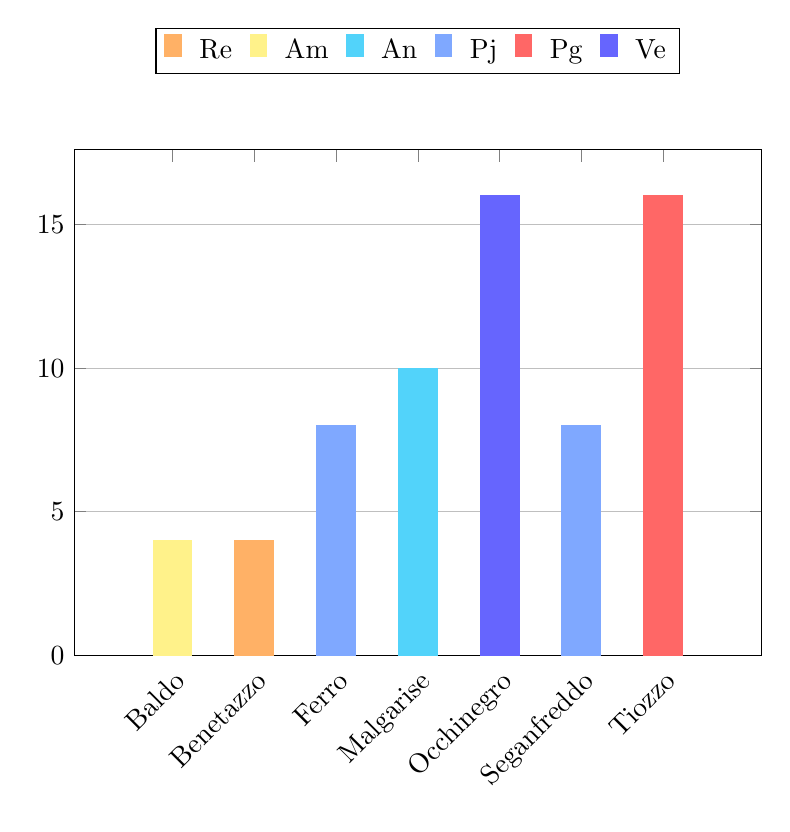
\begin{tikzpicture}
		\begin{axis}[
			width  = 0.85*\textwidth,
			height = 8cm,
			ybar stacked,
			bar width=14pt,
			ymajorgrids = true,
			symbolic x coords={Baldo, Benetazzo, Ferro, Malgarise, Occhinegro, Seganfreddo, Tiozzo},
			xtick = data,
			scaled y ticks = false,
			enlarge x limits=0.2,
			ymin=0,
			legend cell align=left,
			legend style={
				at={(0.5,1.15)},
				anchor=south,
				column sep=1ex,
				legend columns=-1
			},
			xticklabel style={rotate=45, anchor=north east, yshift=0ex, xshift=0ex},
		]
			\addplot+[ybar, resp, fill=resp, mark=none] plot coordinates {
				(Baldo, 0)
				(Benetazzo, 4)
				(Ferro, 0)
				(Malgarise, 0)
				(Occhinegro, 0)
				(Seganfreddo, 0)
				(Tiozzo, 0)
			};
			\addplot+[ybar, amm, fill=amm, mark=none] plot coordinates {
				(Baldo, 4)
				(Benetazzo, 0)
				(Ferro, 0)
				(Malgarise, 0)
				(Occhinegro, 0)
				(Seganfreddo, 0)
				(Tiozzo, 0)
			};
			\addplot+[ybar, an, fill=an, mark=none] plot coordinates {
				(Baldo, 0)
				(Benetazzo, 0)
				(Ferro, 0)
				(Malgarise, 10)
				(Occhinegro, 0)
				(Seganfreddo, 0)
				(Tiozzo, 0)
			};
			\addplot+[ybar, pj, fill=pj, mark=none] plot coordinates {
				(Baldo, 0)
				(Benetazzo, 0)
				(Ferro, 8)
				(Malgarise, 0)
				(Occhinegro, 0)
				(Seganfreddo, 8)
				(Tiozzo, 0)
			};
			\addplot+[ybar, pg, fill=pg, mark=none] plot coordinates {
				(Baldo, 0)
				(Benetazzo, 0)
				(Ferro, 0)
				(Malgarise, 0)
				(Occhinegro, 0)
				(Seganfreddo, 0)
				(Tiozzo, 16)
			};
			\addplot+[ybar, ver, fill=ver, mark=none] plot coordinates {
				(Baldo, 0)
				(Benetazzo, 0)
				(Ferro, 0)
				(Malgarise, 0)
				(Occhinegro, 16)
				(Seganfreddo, 0)
				(Tiozzo, 0)
			};
			\legend{Re, Am, An, Pj, Pg, Ve}
		\end{axis}
	\end{tikzpicture}
	\caption{Impegno preventivo per ruolo dei membri del team durante il nono \href{https://7last.github.io/docs/pb/documentazione-interna/glossario\#sprint}{sprint\textsubscript{G}}}

\end{figure}

%---------1_GRAFICO A TORTA-----------%
\begin{figure}[!h]
	\centering
	\begin{tikzpicture}
		\def\printonlypositive#1{\ifdim#1pt>0pt#1\%\else\fi}
		\pie[pos={8,0},radius=3.5,text=legend,
			before number=\printonlypositive, after number=, color={resp,amm,an,pj,pg,ver}] {
			6.1/\href{https://7last.github.io/docs/pb/documentazione-interna/glossario\#responsabile}{Responsabile\textsubscript{G}},
			6.1/\href{https://7last.github.io/docs/pb/documentazione-interna/glossario\#amministratore}{Amministratore\textsubscript{G}},
			15.2/\href{https://7last.github.io/docs/pb/documentazione-interna/glossario\#analista}{Analista\textsubscript{G}},
			24.2/\href{https://7last.github.io/docs/pb/documentazione-interna/glossario\#progettista}{Progettista\textsubscript{G}},
			24.2/\href{https://7last.github.io/docs/pb/documentazione-interna/glossario\#programmatore}{Programmatore\textsubscript{G}},
			24.2/\href{https://7last.github.io/docs/pb/documentazione-interna/glossario\#verificatore}{Verificatore\textsubscript{G}}
		}
	\end{tikzpicture}
	\caption{Ripartizione in percentuale dei ruoli nel nono \href{https://7last.github.io/docs/pb/documentazione-interna/glossario\#sprint}{sprint\textsubscript{G}}}

\end{figure}

\newpage
\subsubsubsection{Consuntivo}
A causa degli esami universitari e di altri impegni personali, il gruppo non è riuscito ad ultimare tutte le attività pianificate per questo periodo. Queste verranno portate a termine con priorità massima nel prossimo \href{https://7last.github.io/docs/pb/documentazione-interna/glossario\#sprint}{sprint\textsubscript{G}}.

\subsubsubsubsection{Prospetto orario} 
\begin{table}[!h]
    \centering
    \begin{tabular}{ | l | c | c | c | c | c | c | c | }
        \hline
		\textbf{} & \textbf{Re} & \textbf{Am} &\textbf{An} & \textbf{Pj} & \textbf{Pg} & \textbf{Ve} & \textbf{Totale per persona} \\
		\hline			    %RE    %AM    %AN    %PJ   %PG     %VE   %TOT
		Baldo            &  -   &  4   &  -   &  -   &  -   &  -   &  4   \\
		Benetazzo        &  4   &  -   &  -   &  -   &  -   &  -   &  4   \\
		Ferro            &  -   &  -   &  -   &  6   &  -   &  -   &  6   \\
		Malgarise        &  -   &  -   &  9,5 &  -   &  -   &  -   &  9,5 \\
		Occhinegro       &  -   &  -   &  -   &  -   &  -   & 16   & 16   \\
		Seganfreddo      &  -   &  -   &  -   &  8   &  -   &  -   &  8   \\
		Tiozzo           &  -   &  -   &  -   &  -   & 14   &  -   & 14   \\
		\hline
		Totale per ruolo &  4   &  4   &  9,5 & 14   & 14   & 16   &  -   \\
		\hline
    \end{tabular}
    \caption{Consuntivo orario per ruolo dei membri del team durante il nono \href{https://7last.github.io/docs/pb/documentazione-interna/glossario\#sprint}{sprint\textsubscript{G}}}
\end{table}

\newpage
\subsubsubsubsection{Prospetto economico} 
\begin{table}[!h]
    \centering
    \begin{tabular}{ | l | c | c | c | c | c | }
        \hline
        \textbf{Ruolo} & \textbf{Ore} & \textbf{Costo} & \textbf{Ore rimanenti preventivo} & \textbf{Ore rimanenti consuntivo} \\
        \hline
        \href{https://7last.github.io/docs/pb/documentazione-interna/glossario\#responsabile}{Responsabile\textsubscript{G}}     &  4   &  120,00 € &  17   &  17   \\
        \href{https://7last.github.io/docs/pb/documentazione-interna/glossario\#amministratore}{Amministratore\textsubscript{G}} &  4   &   80,00 € &  11   &  11   \\
        \href{https://7last.github.io/docs/pb/documentazione-interna/glossario\#analista}{Analista\textsubscript{G}}             &  9,5 &  237,50 € &  -1,5 &  -1   \\
        \href{https://7last.github.io/docs/pb/documentazione-interna/glossario\#progettista}{Progettista\textsubscript{G}}       & 14   &  350,00 € &  47   &  49   \\
        \href{https://7last.github.io/docs/pb/documentazione-interna/glossario\#programmatore}{Programmatore\textsubscript{G}}   & 14   &  210,00 € &  64,5 &  66,5 \\
        \href{https://7last.github.io/docs/pb/documentazione-interna/glossario\#verificatore}{Verificatore\textsubscript{G}}     & 16   &  240,00 € &  91   &  91   \\
        \hline
        \textbf{Totale preventivo} &  66   & 1330,00 € & 229   &    -   \\
        \hline
        \textbf{Totale consuntivo} &  61,5 & 1237,50 € &   -   &  233,5 \\
        \hline
    \end{tabular}
    \caption{Consuntivo economico durante il nono \href{https://7last.github.io/docs/pb/documentazione-interna/glossario\#sprint}{sprint\textsubscript{G}}}

\end{table}

\subsubsubsubsection{Rischi effettivamente occorsi e loro mitigazione}
\begin{table}[!h]
    \centering
    \begin{tabular}{ | p{6cm} | p{2.5cm} | p{7.5cm} | }
        \hline
        \textbf{Tipologia} & \textbf{Rischio preventivato} & \textbf{Mitigazione}  \\
        \hline
        Impegni personali o universitari (Rischio \textbf{RO-2})& SI & Comunicato in anticipo gli impegni, lavoro affidato svolto prima o dopo l’impegno. \\
        \hline
		Ritardi rispetto alle tempistiche previste (Rischio \textbf{RO-3}) & SI & Completeremo nel prossimo \href{https://7last.github.io/docs/pb/documentazione-interna/glossario\#sprint}{sprint\textsubscript{G}} le attività non ancora ultimate. \\
        \hline
    \end{tabular}
    \caption{Rischi effettivamente occorsi e loro mitigazione durante il nono \href{https://7last.github.io/docs/pb/documentazione-interna/glossario\#sprint}{sprint\textsubscript{G}}}
\end{table}

\subsubsubsection{Retrospettiva}
Entrambi i rischi preventivati per questo periodo si sono verificati. Nonostante l'attenta pianificazione e la previsione dei rischi occorsi, il gruppo ha comunque avuto ritardi. Tenendo conto di questo problema occorso, provederemo a porre maggiore attenzione nella pianificazione dei prossimi \href{https://7last.github.io/docs/pb/documentazione-interna/glossario\#sprint}{sprint\textsubscript{G}}.

\newpage
\subsubsection{Decimo sprint}
\begin{itemize}
    \item Inizio: 2024-06-27
    \item Fine: 2024-07-03
    \item Fine attuale: 2024-07-03
    \item Giorni di ritardo: nessuno
\end{itemize}

\subsubsubsection{Pianificazione}
Oltre a dover completare le attività rimanenti dal periodo precedente, prevediamo di implementare gli alert mancanti, il calcolo dell'efficienza delle colonnine di ricarica mediante l'utilizzo di \textit{Apache Flink} e relativi grafici nelle \href{https://7last.github.io/docs/pb/documentazione-interna/glossario\#dashboard}{dashboard\textsubscript{G}} di \href{https://7last.github.io/docs/pb/documentazione-interna/glossario\#grafana}{\textit{Grafana}\textsubscript{G}}. Verranno inoltre introdotti i test mancanti nel documento \href{https://7last.github.io/docs/pb/documentazione-interna/glossario\#norme-di-progetto}{\textit{Norme di Progetto}\textsubscript{G}}, oltre a completare la stesura dei documenti \textit{Specifica Tecnica} e \textit{Manuale Utente} e al consueto aggiornamento della documentazione ordinaria (\href{https://7last.github.io/docs/pb/documentazione-interna/glossario\#piano-di-progetto}{PdP\textsubscript{G}}, \href{https://7last.github.io/docs/pb/documentazione-interna/glossario\#piano-di-qualifica}{PdQ\textsubscript{G}}, \href{https://7last.github.io/docs/pb/documentazione-interna/glossario\#glossario}{Glo\textsubscript{G}}, verbali).

\subsubsubsubsection{Rischi attesi}
I rischi attesi per questo periodo sono:
\begin{itemize}
    \item Impegni personali o universitari (RO-2);
	\item ritardi rispetto alle tempistiche previste (RO-3).
\end{itemize}
La sessione estiva è ancora in corso, ci attendiamo quindi i medesimi rischi degli \href{https://7last.github.io/docs/pb/documentazione-interna/glossario\#sprint}{sprint\textsubscript{G}} precedenti ma contiamo di riuscire a gestirli senza ulteriori ritardi.

\newpage
\subsubsubsection{Preventivo}
Ruoli coinvolti: \href{https://7last.github.io/docs/pb/documentazione-interna/glossario\#responsabile}{Responsabile\textsubscript{G}} (Re), \href{https://7last.github.io/docs/pb/documentazione-interna/glossario\#amministratore}{Amministratore\textsubscript{G}} (Am), \href{https://7last.github.io/docs/pb/documentazione-interna/glossario\#analista}{Analista\textsubscript{G}} (An), \href{https://7last.github.io/docs/pb/documentazione-interna/glossario\#progettista}{Progettista\textsubscript{G}} (Pj), \href{https://7last.github.io/docs/pb/documentazione-interna/glossario\#programmatore}{Programmatore\textsubscript{G}} (Pg), \href{https://7last.github.io/docs/pb/documentazione-interna/glossario\#verificatore}{Verificatore\textsubscript{G}} (Ve).
\begin{table}[!h]
    \centering
    \begin{tabular}{ | l | c | c | c | c | c | c | c | }
        \hline
        \textbf{} & \textbf{Re} & \textbf{Am} &\textbf{An} & \textbf{Pj} & \textbf{Pg} & \textbf{Ve} & \textbf{Totale per persona} \\
        \hline
        Baldo            &  -   &  -   &  -   &  8   &  -   &  -   &  8   \\
        Benetazzo        &  -   &  -   &  8   &  -   &  -   &  -   &  8   \\
        Ferro            &  -   &  -   &  -   &  -   & 16   &  -   & 16   \\
        Malgarise        &  -   &  -   &  -   &  8   &  -   &  -   &  8   \\
        Occhinegro       &  4   &  -   &  -   &  -   &  -   &  -   &  4   \\
        Seganfreddo      &  -   &  -   &  -   &  -   &  -   & 16   & 16   \\
        Tiozzo           &  -   &  4   &  -   &  -   &  -   &  -   &  4   \\
        \hline
        Totale per ruolo &  4   &  4   &  8   & 16   & 16   & 16   &  -   \\
        \hline
    \end{tabular}
    \caption{Preventivo orario per ruolo dei membri del team durante il decimo \href{https://7last.github.io/docs/pb/documentazione-interna/glossario\#sprint}{sprint\textsubscript{G}}}
    
\end{table}

%---------1_ISTOGRAMMA-----------%
\begin{figure}[!h]
    \centering
    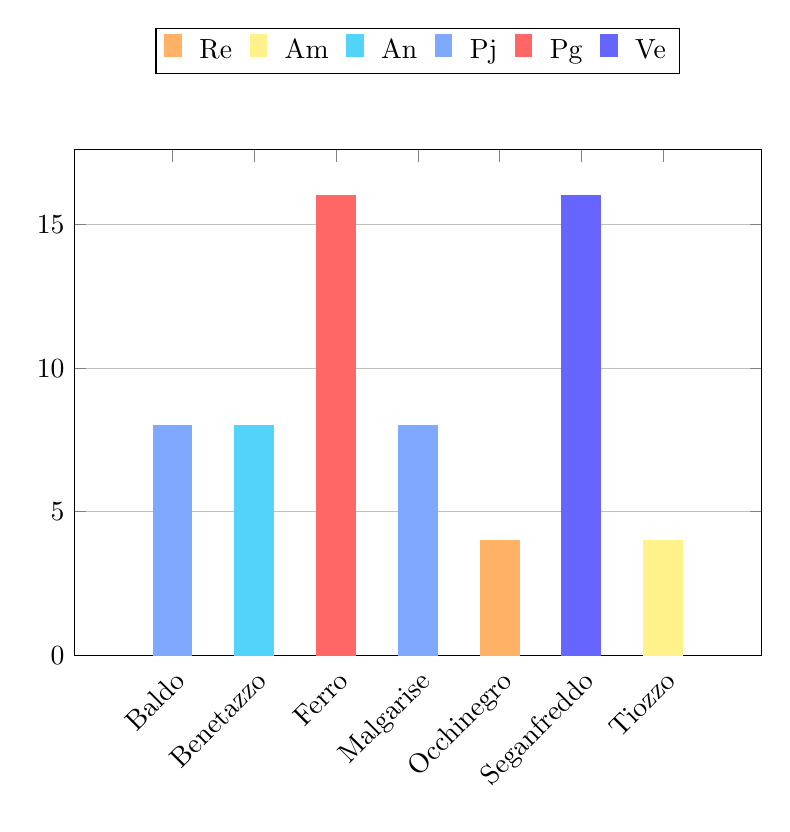
\begin{tikzpicture}
        \begin{axis}[
            width  = 0.85*\textwidth,
            height = 8cm,
            ybar stacked,
            bar width=14pt,
            ymajorgrids = true,
            symbolic x coords={Baldo, Benetazzo, Ferro, Malgarise, Occhinegro, Seganfreddo, Tiozzo},
            xtick = data,
            scaled y ticks = false,
            enlarge x limits=0.2,
            ymin=0,
            legend cell align=left,
            legend style={
                at={(0.5,1.15)},
                anchor=south,
                column sep=1ex,
                legend columns=-1
            },
            xticklabel style={rotate=45, anchor=north east, yshift=0ex, xshift=0ex},
            ]
            \addplot+[ybar, resp, fill=resp, mark=none] plot coordinates {
                (Baldo, 0)
                (Benetazzo, 0)
                (Ferro, 0)
                (Malgarise, 0)
                (Occhinegro, 4)
                (Seganfreddo, 0)
                (Tiozzo, 0)
            };
            \addplot+[ybar, amm, fill=amm, mark=none] plot coordinates {
                (Baldo, 0)
                (Benetazzo, 0)
                (Ferro, 0)
                (Malgarise, 0)
                (Occhinegro, 0)
                (Seganfreddo, 0)
                (Tiozzo, 4)
            };
            \addplot+[ybar, an, fill=an, mark=none] plot coordinates {
                (Baldo, 0)
                (Benetazzo, 8)
                (Ferro, 0)
                (Malgarise, 0)
                (Occhinegro, 0)
                (Seganfreddo, 0)
                (Tiozzo, 0)
            };
            \addplot+[ybar, pj, fill=pj, mark=none] plot coordinates {
                (Baldo, 8)
                (Benetazzo, 0)
                (Ferro, 0)
                (Malgarise, 8)
                (Occhinegro, 0)
                (Seganfreddo, 0)
                (Tiozzo, 0)
            };
            \addplot+[ybar, pg, fill=pg, mark=none] plot coordinates {
                (Baldo, 0)
                (Benetazzo, 0)
                (Ferro, 16)
                (Malgarise, 0)
                (Occhinegro, 0)
                (Seganfreddo, 0)
                (Tiozzo, 0)
            };
            \addplot+[ybar, ver, fill=ver, mark=none] plot coordinates {
                (Baldo, 0)
                (Benetazzo, 0)
                (Ferro, 0)
                (Malgarise, 0)
                (Occhinegro, 0)
                (Seganfreddo, 16)
                (Tiozzo, 0)
            };
            \legend{Re, Am, An, Pj, Pg, Ve}
        \end{axis}
    \end{tikzpicture}
    \caption{Impegno preventivo per ruolo dei membri del team durante il decimo \href{https://7last.github.io/docs/pb/documentazione-interna/glossario\#sprint}{sprint\textsubscript{G}}}
    
\end{figure}

%---------1_GRAFICO A TORTA-----------%
\begin{figure}[!h]
    \centering
    \begin{tikzpicture}
        \def\printonlypositive#1{\ifdim#1pt>0pt
        #1
        \fi}
        \pie[pos={8,0},radius=3.5,text=legend,
        before number=\printonlypositive,color={resp,amm,an,pj,pg,ver}] {
             6.3/\href{https://7last.github.io/docs/pb/documentazione-interna/glossario\#responsabile}{Responsabile\textsubscript{G}},
             6.3/\href{https://7last.github.io/docs/pb/documentazione-interna/glossario\#amministratore}{Amministratore\textsubscript{G}},
             12.5/\href{https://7last.github.io/docs/pb/documentazione-interna/glossario\#analista}{Analista\textsubscript{G}},
             25.0/\href{https://7last.github.io/docs/pb/documentazione-interna/glossario\#progettista}{Progettista\textsubscript{G}},
             25.0/\href{https://7last.github.io/docs/pb/documentazione-interna/glossario\#programmatore}{Programmatore\textsubscript{G}},
             25.0/\href{https://7last.github.io/docs/pb/documentazione-interna/glossario\#verificatore}{Verificatore\textsubscript{G}}
        }
        \end{tikzpicture}
    \caption{Ripartizione in percentuale dei ruoli nel decimo \href{https://7last.github.io/docs/pb/documentazione-interna/glossario\#sprint}{sprint\textsubscript{G}}}
\end{figure}

\subsubsubsection{Consuntivo}
Nonostante qualche difficoltà nella configurazione ed utilizzo di \textit{Apache Flink} siamo riusciti a completare tutte le attività entro le scadenze prefissate. Rispetto al preventivo sono servite meno ore al \href{https://7last.github.io/docs/pb/documentazione-interna/glossario\#programmatore}{programmatore\textsubscript{G}}, mentre le attività dei \href{https://7last.github.io/docs/pb/documentazione-interna/glossario\#progettista}{progettisti\textsubscript{G}} si sono rilevate particolarmente impegnative, richiedendo più ore di quelle previste. Nel complesso siamo comunque riusciti a rimanere entro il budget preventivato per questo periodo.

\subsubsubsubsection{Prospetto orario}
\begin{table}[!h]
    \centering
    \begin{tabular}{ | l | c | c | c | c | c | c | c | }
        \hline
        \textbf{} & \textbf{Re} & \textbf{Am} &\textbf{An} & \textbf{Pj} & \textbf{Pg} & \textbf{Ve} & \textbf{Totale per persona} \\
        \hline
        Baldo            &  -   &  -   &  -   &  9,5 &  -   &  -   &  9,5 \\
        Benetazzo        &  -   &  -   &  7   &  -   &  -   &  -   &  7   \\
        Ferro            &  -   &  -   &  -   &  -   & 12   &  -   & 12   \\
        Malgarise        &  -   &  -   &  -   &  8,5 &  -   &  -   &  8,5 \\
        Occhinegro       &  4   &  -   &  -   &  -   &  -   &  -   &  4   \\
        Seganfreddo      &  -   &  -   &  -   &  -   &  -   & 14   & 14   \\
        Tiozzo           &  -   &  3,5 &  -   &  -   &  -   &  -   &  3,5 \\
        \hline
        Totale per ruolo &  4   &  3,5 &  7   & 18   & 12   & 14   &  -   \\
        \hline
    \end{tabular}
    \caption{Consuntivo orario per ruolo dei membri del team durante il decimo \href{https://7last.github.io/docs/pb/documentazione-interna/glossario\#sprint}{sprint\textsubscript{G}}}
\end{table}

\newpage
\subsubsubsubsection{Prospetto economico}
\begin{table}[!h]
    \centering
    \begin{tabular}{ | l | c | c | c | c | c | }
        \hline
        \textbf{Ruolo} & \textbf{Ore} & \textbf{Costo} & \textbf{Ore rimanenti preventivo} & \textbf{Ore rimanenti consuntivo} \\
        \hline
        \href{https://7last.github.io/docs/pb/documentazione-interna/glossario\#responsabile}{Responsabile\textsubscript{G}}     &  4   &  120,00 € &  13   &  13   \\
        \href{https://7last.github.io/docs/pb/documentazione-interna/glossario\#amministratore}{Amministratore\textsubscript{G}} &  3,5 &   70,00 € &   7   &   7,5 \\
        \href{https://7last.github.io/docs/pb/documentazione-interna/glossario\#analista}{Analista\textsubscript{G}}             &  7   &  175,00 € &  -9   &  -8   \\
        \href{https://7last.github.io/docs/pb/documentazione-interna/glossario\#progettista}{Progettista\textsubscript{G}}       & 18   &  450,00 € &  33   &  31   \\
        \href{https://7last.github.io/docs/pb/documentazione-interna/glossario\#programmatore}{Programmatore\textsubscript{G}}   & 12   &  180,00 € &  50,5 &  54,5 \\
        \href{https://7last.github.io/docs/pb/documentazione-interna/glossario\#verificatore}{Verificatore\textsubscript{G}}     & 14   &  210,00 € &  75   &  77   \\
        \hline
        \textbf{Totale preventivo} & 64   & 1280,00 € & 169,5 &   -   \\
        \hline
        \textbf{Totale consuntivo} & 58,5 & 1205,00 € &   -   & 175   \\
        \hline
    \end{tabular}
    \caption{Consuntivo economico durante il decimo \href{https://7last.github.io/docs/pb/documentazione-interna/glossario\#sprint}{sprint\textsubscript{G}}}
\end{table}

\subsubsubsubsection{Rischi effettivamente occorsi e loro mitigazione}
\begin{table}[!h]
    \centering
    \begin{tabular}{ | p{6cm} | p{2.5cm} | p{7.5cm} | }
        \hline
        \textbf{Tipologia} & \textbf{Rischio preventivato} & \textbf{Mitigazione}  \\
        \hline
        Impegni personali o universitari (Rischio \textbf{RO-2})& SI & Comunicato in anticipo gli impegni, lavoro affidato svolto prima o dopo l'impegno.\\
        \hline
    \end{tabular}
    \caption{Rischi effettivamente occorsi e loro mitigazione durante il decimo \href{https://7last.github.io/docs/pb/documentazione-interna/glossario\#sprint}{sprint\textsubscript{G}}}
\end{table}

\subsubsubsection{Retrospettiva}
Questo periodo si è concluso senza ritardi e con tutte le attività completate. Il gruppo ha lavorato in modo efficiente e coordinato, evitando che gli impegni universitari potessero causare ulteriori ritardi, grazie ad un'attenta pianificazione delle attività e in alcuni casi ad una riassegnazione dei compiti da svolgere, in modo che chi fosse in difficoltà potesse essere aiutato da chi aveva più tempo a disposizione.


\newpage
\subsubsection{Undicesimo sprint}
\begin{itemize}
    \item Inizio: 2024-07-04
    \item Fine: 2024-07-10
    \item Fine attuale: 2024-07-10
    \item Giorni di ritardo: nessuno
\end{itemize}

\subsubsubsection{Pianificazione}
Le attività pianificate prevedono l'implementazione dei test di integrazione, la riprogettazione delle \href{https://7last.github.io/docs/pb/documentazione-interna/glossario\#dashboard}{dashboard\textsubscript{G}} secondo le indicazioni del \href{https://7last.github.io/docs/pb/documentazione-interna/glossario\#proponente}{proponente\textsubscript{G}}, ovvero separando i dati grezzi o in \textit{real time} da quelli aggregati e analitici (in modo da rendere le \href{https://7last.github.io/docs/pb/documentazione-interna/glossario\#dashboard}{\textit{dashboard}\textsubscript{G}} più leggibili e fruibili da parte degli utenti). Per quanto riguarda la documentazione verranno aggiornati i documenti \href{https://7last.github.io/docs/pb/documentazione-interna/glossario\#piano-di-progetto}{\textit{Piano di Progetto}\textsubscript{G}} e \href{https://7last.github.io/docs/pb/documentazione-interna/glossario\#piano-di-qualifica}{\textit{Piano di Qualifica}\textsubscript{G}}.

\subsubsubsubsection{Rischi attesi}
I rischi attesi per questo periodo sono:
\begin{itemize}
    \item impegni personali o universitari (RO-2);
	\item ritardi rispetto alle tempistiche previste (RO-3).
\end{itemize}
Ci attendiamo che possano occorrere i medesimi rischi degli \href{https://7last.github.io/docs/pb/documentazione-interna/glossario\#sprint}{sprint\textsubscript{G}} passati.

\newpage
\subsubsubsection{Preventivo}
Ruoli coinvolti: \href{https://7last.github.io/docs/pb/documentazione-interna/glossario\#responsabile}{Responsabile\textsubscript{G}} (Re), \href{https://7last.github.io/docs/pb/documentazione-interna/glossario\#amministratore}{Amministratore\textsubscript{G}} (Am), \href{https://7last.github.io/docs/pb/documentazione-interna/glossario\#progettista}{Progettista\textsubscript{G}} (Pj), \href{https://7last.github.io/docs/pb/documentazione-interna/glossario\#programmatore}{Programmatore\textsubscript{G}} (Pg), \href{https://7last.github.io/docs/pb/documentazione-interna/glossario\#verificatore}{Verificatore\textsubscript{G}} (Ve).
\begin{table}[!h]
    \centering
    \begin{tabular}{ | l | c | c | c | c | c | c | c | }
        \hline
        \textbf{} & \textbf{Re} & \textbf{Am} &\textbf{An} & \textbf{Pj} & \textbf{Pg} & \textbf{Ve} & \textbf{Totale per persona} \\
        \hline
        Baldo            &  -   &  -   &  -   &  8   &  -   &  -   &  8   \\
        Benetazzo        &  -   &  -   &  -   &  -   & 12   &  -   & 12   \\
        Ferro            &  -   &  -   &  -   &  -   &  -   &  8   &  8   \\
        Malgarise        &  -   &  -   &  -   &  -   &  -   &  8   &  8   \\
        Occhinegro       &  -   &  4   &  -   &  -   &  -   &  -   &  4   \\
        Seganfreddo      &  4   &  -   &  -   &  -   &  -   &  -   &  4   \\
        Tiozzo           &  -   &  -   &  -   &  8   &  -   &  -   &  8   \\
        \hline
        Totale per ruolo &  4   &  4   &  -   & 16   & 12   & 16   &  -   \\
        \hline
    \end{tabular}
    \caption{Preventivo orario per ruolo dei membri del team durante l'undicesimo \href{https://7last.github.io/docs/pb/documentazione-interna/glossario\#sprint}{sprint\textsubscript{G}}}
    
\end{table}

%---------1_ISTOGRAMMA-----------%
\begin{figure}[!h]
    \centering
    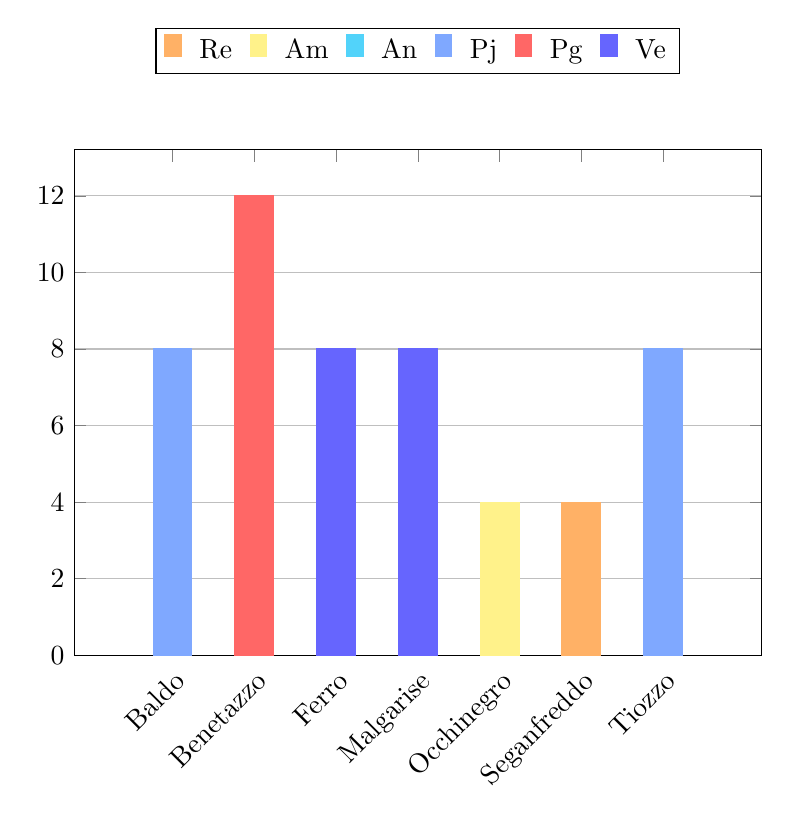
\begin{tikzpicture}
        \begin{axis}[
            width  = 0.85*\textwidth,
            height = 8cm,
            ybar stacked,
            bar width=14pt,
            ymajorgrids = true,
            symbolic x coords={Baldo, Benetazzo, Ferro, Malgarise, Occhinegro, Seganfreddo, Tiozzo},
            xtick = data,
            scaled y ticks = false,
            enlarge x limits=0.2,
            ymin=0,
            legend cell align=left,
            legend style={
                at={(0.5,1.15)},
                anchor=south,
                column sep=1ex,
                legend columns=-1
            },
            xticklabel style={rotate=45, anchor=north east, yshift=0ex, xshift=0ex},
            ]
            \addplot+[ybar, resp, fill=resp, mark=none] plot coordinates {
                (Baldo, 0)
                (Benetazzo, 0)
                (Ferro, 0)
                (Malgarise, 0)
                (Occhinegro, 0)
                (Seganfreddo, 4)
                (Tiozzo, 0)
            };
            \addplot+[ybar, amm, fill=amm, mark=none] plot coordinates {
                (Baldo, 0)
                (Benetazzo, 0)
                (Ferro, 0)
                (Malgarise, 0)
                (Occhinegro, 4)
                (Seganfreddo, 0)
                (Tiozzo, 0)
            };
            \addplot+[ybar, an, fill=an, mark=none] plot coordinates {
                (Baldo, 0)
                (Benetazzo, 0)
                (Ferro, 0)
                (Malgarise, 0)
                (Occhinegro, 0)
                (Seganfreddo, 0)
                (Tiozzo, 0)
            };
            \addplot+[ybar, pj, fill=pj, mark=none] plot coordinates {
                (Baldo, 8)
                (Benetazzo, 0)
                (Ferro, 0)
                (Malgarise, 0)
                (Occhinegro, 0)
                (Seganfreddo, 0)
                (Tiozzo, 8)
            };
            \addplot+[ybar, pg, fill=pg, mark=none] plot coordinates {
                (Baldo, 0)
                (Benetazzo, 12)
                (Ferro, 0)
                (Malgarise, 0)
                (Occhinegro, 0)
                (Seganfreddo, 0)
                (Tiozzo, 0)
            };
            \addplot+[ybar, ver, fill=ver, mark=none] plot coordinates {
                (Baldo, 0)
                (Benetazzo, 0)
                (Ferro, 8)
                (Malgarise, 8)
                (Occhinegro, 0)
                (Seganfreddo, 0)
                (Tiozzo, 0)
            };
            \legend{Re, Am, An, Pj, Pg, Ve}
        \end{axis}
    \end{tikzpicture}
    \caption{Impegno preventivo per ruolo dei membri durante l'undicesimo \href{https://7last.github.io/docs/pb/documentazione-interna/glossario\#sprint}{sprint\textsubscript{G}}}
    
\end{figure}

%---------1_GRAFICO A TORTA-----------%
\begin{figure}[!h]
    \centering
    \begin{tikzpicture}
        \def\printonlypositive#1{\ifdim#1pt>0pt
        #1
        \fi}
        \pie[pos={8,0},radius=3.5,text=legend,
        before number=\printonlypositive,color={resp,amm,pj,pg,ver}] {
             7.7/\href{https://7last.github.io/docs/pb/documentazione-interna/glossario\#responsabile}{Responsabile\textsubscript{G}},
             7.7/\href{https://7last.github.io/docs/pb/documentazione-interna/glossario\#amministratore}{Amministratore\textsubscript{G}},
             30.8/\href{https://7last.github.io/docs/pb/documentazione-interna/glossario\#progettista}{Progettista\textsubscript{G}},
             23.1/\href{https://7last.github.io/docs/pb/documentazione-interna/glossario\#programmatore}{Programmatore\textsubscript{G}},
             30.8/\href{https://7last.github.io/docs/pb/documentazione-interna/glossario\#verificatore}{Verificatore\textsubscript{G}}
        }
        \end{tikzpicture}
    \caption{Ripartizione in percentuale dei ruoli nell'undicesimo \href{https://7last.github.io/docs/pb/documentazione-interna/glossario\#sprint}{sprint\textsubscript{G}}}
\end{figure}

\subsubsubsection{Consuntivo}
Anche questo \href{https://7last.github.io/docs/pb/documentazione-interna/glossario\#sprint}{sprint\textsubscript{G}} si è concluso senza ritardi e con tutte le attività completate. Ci avviciniamo alla fine del progetto e le attività da svolgere cominciano a diminuire. Le ore preventivate si sono rivelate adeguate, siamo quindi riusciti a rimanere entro il budget anche per questo \href{https://7last.github.io/docs/pb/documentazione-interna/glossario\#sprint}{sprint\textsubscript{G}}. 
Considerando i ritardi avvenuti e l'andamento generale degli \href{https://7last.github.io/docs/pb/documentazione-interna/glossario\#sprint}{sprint\textsubscript{G}}, il gruppo ha deciso di rivedere il calendario di progetto posticipando la data prevista per la \href{https://7last.github.io/docs/pb/documentazione-interna/glossario\#product-baseline}{Product Baseline\textsubscript{G}}, ripianificandola per il giorno 2024-07-24. A causa di questa ripianificazione, il budget preventivato per effettuare la \href{https://7last.github.io/docs/pb/documentazione-interna/glossario\#customer-acceptance}{Customer Acceptance\textsubscript{G}} non è più sufficiente, quindi il gruppo ha deciso di non effettuarla e di considerare il progetto concluso una volta completata la \href{https://7last.github.io/docs/pb/documentazione-interna/glossario\#product-baseline}{Product Baseline\textsubscript{G}}.

\newpage
\subsubsubsubsection{Prospetto orario}
\begin{table}[!h]
    \centering
    \begin{tabular}{ | l | c | c | c | c | c | c | c | }
        \hline
        \textbf{} & \textbf{Re} & \textbf{Am} &\textbf{An} & \textbf{Pj} & \textbf{Pg} & \textbf{Ve} & \textbf{Totale per persona} \\
        \hline
        Baldo            &  -   &  -   &  -   &  8   &  -   &  -   &  8   \\
        Benetazzo        &  -   &  -   &  -   &  -   & 12,5 &  -   & 12,5 \\
        Ferro            &  -   &  -   &  -   &  -   &  -   &  6   &  6   \\
        Malgarise        &  -   &  -   &  -   &  -   &  -   & 10   & 10   \\
        Occhinegro       &  -   &  3   &  -   &  -   &  -   &  -   &  3   \\
        Seganfreddo      &  4   &  -   &  -   &  -   &  -   &  -   &  4   \\
        Tiozzo           &  -   &  -   &  -   &  7   &  -   &  -   &  7   \\
        \hline
        Totale per ruolo &  4   &  3   &  -   & 15   & 12,5 & 16   &  -   \\
        \hline
    \end{tabular}
    \caption{Consuntivo orario per ruolo dei membri del team durante l'undicesimo \href{https://7last.github.io/docs/pb/documentazione-interna/glossario\#sprint}{sprint\textsubscript{G}}}
\end{table}

\subsubsubsubsection{Prospetto economico}
\begin{table}[!h]
    \centering
    \begin{tabular}{ | l | c | c | c | c | c | }
        \hline
        \textbf{Ruolo} & \textbf{Ore} & \textbf{Costo} & \textbf{Ore rimanenti preventivo} & \textbf{Ore rimanenti consuntivo} \\
        \hline
        \href{https://7last.github.io/docs/pb/documentazione-interna/glossario\#responsabile}{Responsabile\textsubscript{G}}     &  4   &  120,00 € &   9   &   9   \\
        \href{https://7last.github.io/docs/pb/documentazione-interna/glossario\#amministratore}{Amministratore\textsubscript{G}} &  3   &   60,00 € &   3,5 &   4,5 \\
        \href{https://7last.github.io/docs/pb/documentazione-interna/glossario\#analista}{Analista\textsubscript{G}}             &  0   &    0,00 € &  -8   &  -8   \\
        \href{https://7last.github.io/docs/pb/documentazione-interna/glossario\#progettista}{Progettista\textsubscript{G}}       & 15   &  375,00 € &  15   &  16   \\
        \href{https://7last.github.io/docs/pb/documentazione-interna/glossario\#programmatore}{Programmatore\textsubscript{G}}   & 12,5 &  187,50 € &  42,5 &  42   \\
        \href{https://7last.github.io/docs/pb/documentazione-interna/glossario\#verificatore}{Verificatore\textsubscript{G}}     & 16   &  240,00 € &  61   &  61   \\
        \hline
        \textbf{Totale preventivo} & 52   & 1020,00 € & 123   &   -   \\
        \hline
        \textbf{Totale consuntivo} & 50,5 &  982,50 € &   -   & 124,5 \\
        \hline
    \end{tabular}
    \caption{Consuntivo economico durante l'undicesimo \href{https://7last.github.io/docs/pb/documentazione-interna/glossario\#sprint}{sprint\textsubscript{G}}}
\end{table}

\subsubsubsection{Retrospettiva}
Questo \href{https://7last.github.io/docs/pb/documentazione-interna/glossario\#sprint}{sprint\textsubscript{G}} si è concluso senza il verificarsi di nessun rischio, preventivato o meno. Le attività da svolgere cominciano a diminuire in quantità e complessità con l'avvicinarsi della fine del progetto. 


\newpage
\subsubsection{Dodicesimo sprint}
\begin{itemize}
    \item Inizio: 2024-07-11
    \item Fine: 2024-07-17
    \item Fine attuale: 2024-07-17
    \item Giorni di ritardo: nessuno
\end{itemize}

\subsubsubsection{Pianificazione}
Per questo periodo ci impegniamo a completare i test di integrazione iniziati il precedente \href{https://7last.github.io/docs/pb/documentazione-interna/glossario\#sprint}{sprint\textsubscript{G}} e a ultimare le finiture alle \href{https://7last.github.io/docs/pb/documentazione-interna/glossario\#dashboard}{\textit{dashboard}\textsubscript{G}} in vista del collaudo finale. Verrà aggiornato il documento \href{https://7last.github.io/docs/pb/documentazione-interna/glossario\#norme-di-progetto}{\textit{Norme di Progetto}\textsubscript{G}} con l'aggiunta degli ultimi test implementati, oltre al consueto aggiornamento dei documenti \href{https://7last.github.io/docs/pb/documentazione-interna/glossario\#piano-di-progetto}{\textit{Piano di Progetto}\textsubscript{G}} e \href{https://7last.github.io/docs/pb/documentazione-interna/glossario\#piano-di-qualifica}{\textit{Piano di Qualifica}\textsubscript{G}} e alla stesura dei verbali.

\subsubsubsubsection{Rischi attesi}
I rischi attesi per questo periodo sono:
\begin{itemize}
    \item impegni personali o universitari (RO-2);
	\item ritardi rispetto alle tempistiche previste (RO-3).
\end{itemize}

\newpage
\subsubsubsection{Preventivo}
Ruoli coinvolti: \href{https://7last.github.io/docs/pb/documentazione-interna/glossario\#responsabile}{Responsabile\textsubscript{G}} (Re), \href{https://7last.github.io/docs/pb/documentazione-interna/glossario\#amministratore}{Amministratore\textsubscript{G}} (Am), \href{https://7last.github.io/docs/pb/documentazione-interna/glossario\#progettista}{Progettista\textsubscript{G}} (Pj), \href{https://7last.github.io/docs/pb/documentazione-interna/glossario\#programmatore}{Programmatore\textsubscript{G}} (Pg), \href{https://7last.github.io/docs/pb/documentazione-interna/glossario\#verificatore}{Verificatore\textsubscript{G}} (Ve).
\begin{table}[!h]
    \centering
    \begin{tabular}{ | l | c | c | c | c | c | c | c | }
        \hline
        \textbf{} & \textbf{Re} & \textbf{Am} &\textbf{An} & \textbf{Pj} & \textbf{Pg} & \textbf{Ve} & \textbf{Totale per persona} \\
        \hline
        Baldo            &  -   &  -   &  -   &  -   &  -   & 12   & 12   \\
        Benetazzo        &  -   &  -   &  -   &  -   &  -   & 12   & 12   \\
        Ferro            &  4   &  -   &  -   &  -   &  -   &  -   &  4   \\
        Malgarise        &  -   &  -   &  -   &  -   &  8   &  -   &  8   \\
        Occhinegro       &  -   &  -   &  -   &  8   &  -   &  -   &  8   \\
        Seganfreddo      &  -   &  4   &  -   &  -   &  -   &  -   &  4   \\
        Tiozzo           &  -   &  -   &  -   &  -   &  8   &  -   &  8   \\
        \hline
        Totale per ruolo &  4   &  4   &  -   &  8   & 16   & 24   &  -   \\
        \hline
    \end{tabular}
    \caption{Preventivo orario per ruolo dei membri del team durante il dodicesimo \href{https://7last.github.io/docs/pb/documentazione-interna/glossario\#sprint}{sprint\textsubscript{G}}}
    
\end{table}

%---------1_ISTOGRAMMA-----------%
\begin{figure}[!h]
    \centering
    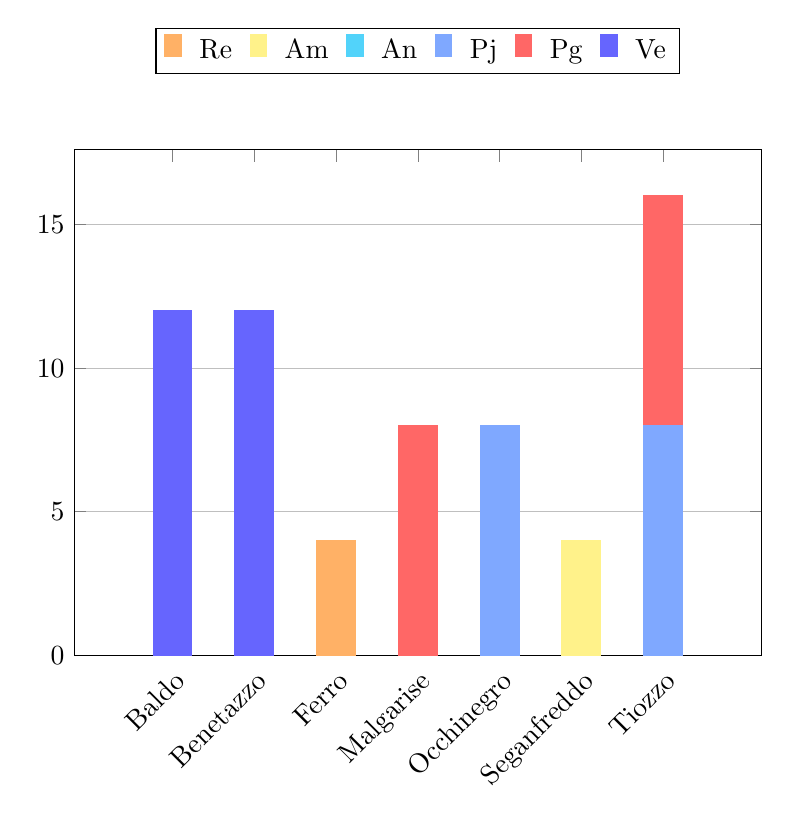
\begin{tikzpicture}
        \begin{axis}[
            width  = 0.85*\textwidth,
            height = 8cm,
            ybar stacked,
            bar width=14pt,
            ymajorgrids = true,
            symbolic x coords={Baldo, Benetazzo, Ferro, Malgarise, Occhinegro, Seganfreddo, Tiozzo},
            xtick = data,
            scaled y ticks = false,
            enlarge x limits=0.2,
            ymin=0,
            legend cell align=left,
            legend style={
                at={(0.5,1.15)},
                anchor=south,
                column sep=1ex,
                legend columns=-1
            },
            xticklabel style={rotate=45, anchor=north east, yshift=0ex, xshift=0ex},
            ]
            \addplot+[ybar, resp, fill=resp, mark=none] plot coordinates {
                (Baldo, 0)
                (Benetazzo, 0)
                (Ferro, 4)
                (Malgarise, 0)
                (Occhinegro, 0)
                (Seganfreddo, 0)
                (Tiozzo, 0)
            };
            \addplot+[ybar, amm, fill=amm, mark=none] plot coordinates {
                (Baldo, 0)
                (Benetazzo, 0)
                (Ferro, 0)
                (Malgarise, 0)
                (Occhinegro, 0)
                (Seganfreddo, 4)
                (Tiozzo, 0)
            };
            \addplot+[ybar, an, fill=an, mark=none] plot coordinates {
                (Baldo, 0)
                (Benetazzo, 0)
                (Ferro, 0)
                (Malgarise, 0)
                (Occhinegro, 0)
                (Seganfreddo, 0)
                (Tiozzo, 0)
            };
            \addplot+[ybar, pj, fill=pj, mark=none] plot coordinates {
                (Baldo, 0)
                (Benetazzo, 0)
                (Ferro, 0)
                (Malgarise, 0)
                (Occhinegro, 8)
                (Seganfreddo, 0)
                (Tiozzo, 8)
            };
            \addplot+[ybar, pg, fill=pg, mark=none] plot coordinates {
                (Baldo, 0)
                (Benetazzo, 0)
                (Ferro, 0)
                (Malgarise, 8)
                (Occhinegro, 0)
                (Seganfreddo, 0)
                (Tiozzo, 8)
            };
            \addplot+[ybar, ver, fill=ver, mark=none] plot coordinates {
                (Baldo, 12)
                (Benetazzo, 12)
                (Ferro, 0)
                (Malgarise, 0)
                (Occhinegro, 0)
                (Seganfreddo, 0)
                (Tiozzo, 0)
            };
            \legend{Re, Am, An, Pj, Pg, Ve}
        \end{axis}
    \end{tikzpicture}
    \caption{Impegno preventivo per ruolo dei membri durante il dodicesimo \href{https://7last.github.io/docs/pb/documentazione-interna/glossario\#sprint}{sprint\textsubscript{G}}}
    
\end{figure}

%---------1_GRAFICO A TORTA-----------%
\begin{figure}[!h]
    \centering
    \begin{tikzpicture}
        \def\printonlypositive#1{\ifdim#1pt>0pt
        #1
        \fi}
        \pie[pos={8,0},radius=3.5,text=legend,
        before number=\printonlypositive,color={resp,amm,pj,pg,ver}] {
             7.0/\href{https://7last.github.io/docs/pb/documentazione-interna/glossario\#responsabile}{Responsabile\textsubscript{G}},
             7.0/\href{https://7last.github.io/docs/pb/documentazione-interna/glossario\#amministratore}{Amministratore\textsubscript{G}},
             14.0/\href{https://7last.github.io/docs/pb/documentazione-interna/glossario\#progettista}{Progettista\textsubscript{G}},
             29.0/\href{https://7last.github.io/docs/pb/documentazione-interna/glossario\#programmatore}{Programmatore\textsubscript{G}},
             43.0/\href{https://7last.github.io/docs/pb/documentazione-interna/glossario\#verificatore}{Verificatore\textsubscript{G}}
        }
        \end{tikzpicture}
    \caption{Ripartizione in percentuale dei ruoli nel dodicesimo \href{https://7last.github.io/docs/pb/documentazione-interna/glossario\#sprint}{sprint\textsubscript{G}}}
\end{figure}

\subsubsubsection{Consuntivo}
Questo \href{https://7last.github.io/docs/pb/documentazione-interna/glossario\#sprint}{sprint\textsubscript{G}}, come preventivato, ha richiesto un maggior impegno da parte dei \href{https://7last.github.io/docs/pb/documentazione-interna/glossario\#verificatore}{verificatori\textsubscript{G}} per le operazioni di verifica in vista del collaudo finale con il \href{https://7last.github.io/docs/pb/documentazione-interna/glossario\#proponente}{proponente\textsubscript{G}}. Le ore preventivate si sono comunque rivelate adeguate per le attività da svolgere, siamo quindi riusciti a rimanere entro il budget previsto per questo periodo.

\subsubsubsubsection{Prospetto orario}
\begin{table}[!h]
    \centering
    \begin{tabular}{ | l | c | c | c | c | c | c | c | }
        \hline
        \textbf{} & \textbf{Re} & \textbf{Am} &\textbf{An} & \textbf{Pj} & \textbf{Pg} & \textbf{Ve} & \textbf{Totale per persona} \\
        \hline
        Baldo            &  -   &  -   &  -   &  -   &  -   &  9   &  9   \\
        Benetazzo        &  -   &  -   &  -   &  -   &  -   & 15,5 & 15,5 \\
        Ferro            &  3   &  -   &  -   &  -   &  -   &  -   &  3   \\
        Malgarise        &  -   &  -   &  -   &  -   &  9   &  -   &  9   \\
        Occhinegro       &  -   &  -   &  -   &  8   &  -   &  -   &  8   \\
        Seganfreddo      &  -   &  2,5 &  -   &  -   &  -   &  -   &  2.5 \\
        Tiozzo           &  -   &  -   &  -   &  -   &  7   &  -   &  7   \\
        \hline
        Totale per ruolo &  3   &  2,5 &  -   &  8   & 16   & 24,5 &  -   \\
        \hline
    \end{tabular}
    \caption{Consuntivo orario per ruolo dei membri durante il dodicesimo \href{https://7last.github.io/docs/pb/documentazione-interna/glossario\#sprint}{sprint\textsubscript{G}}}
\end{table}

\newpage
\subsubsubsubsection{Prospetto economico}
\begin{table}[!h]
    \centering
    \begin{tabular}{ | l | c | c | c | c | c | }
        \hline
        \textbf{Ruolo} & \textbf{Ore} & \textbf{Costo} & \textbf{Ore rimanenti preventivo} & \textbf{Ore rimanenti consuntivo} \\
        \hline
        \href{https://7last.github.io/docs/pb/documentazione-interna/glossario\#responsabile}{Responsabile\textsubscript{G}}     &  3   &   90,00 € &   5   &   6   \\
        \href{https://7last.github.io/docs/pb/documentazione-interna/glossario\#amministratore}{Amministratore\textsubscript{G}} &  2,5 &   50,00 € &   0,5 &   2   \\
        \href{https://7last.github.io/docs/pb/documentazione-interna/glossario\#analista}{Analista\textsubscript{G}}             &  0   &    0,00 € &  -8   &  -8   \\
        \href{https://7last.github.io/docs/pb/documentazione-interna/glossario\#progettista}{Progettista\textsubscript{G}}       &  8   &  200,00 € &   8   &   8   \\
        \href{https://7last.github.io/docs/pb/documentazione-interna/glossario\#programmatore}{Programmatore\textsubscript{G}}   & 16   &  240,00 € &  26   &  26   \\
        \href{https://7last.github.io/docs/pb/documentazione-interna/glossario\#verificatore}{Verificatore\textsubscript{G}}     & 24,5 &  367,50 € &  37   &  36,5 \\
        \hline
        \textbf{Totale preventivo} & 56   & 1000,00 € &  68,5 &   -   \\
        \hline
        \textbf{Totale consuntivo} & 54   &  947,50 € &   -   &  70,5 \\
        \hline
    \end{tabular}
    \caption{Consuntivo economico durante il dodicesimo \href{https://7last.github.io/docs/pb/documentazione-interna/glossario\#sprint}{sprint\textsubscript{G}}}
\end{table}

\subsubsubsection{Retrospettiva}
Anche questo \href{https://7last.github.io/docs/pb/documentazione-interna/glossario\#sprint}{sprint\textsubscript{G}} si è concluso senza l'insorgere di rischi, né tra quelli preventivati né tra quelli non preventivati. Siamo riusciti a raggiungere un livello di maturazione sul prodotto che possiamo considerare soddisfacente per un possibile \href{https://7last.github.io/docs/pb/documentazione-interna/glossario\#minimum-viable-product}{\textit{Minimum Viable Product}\textsubscript{G}}. Attendiamo il riscontro da parte del \href{https://7last.github.io/docs/pb/documentazione-interna/glossario\#proponente}{proponente\textsubscript{G}} in occasione del collaudo finale previsto per il giorno 2024-07-19.

\newpage
\subsubsection{Tredicesimo sprint}
\begin{itemize}
    \item Inizio: 2024-07-18
    \item Fine: 2024-07-24
    \item Fine attuale: 2024-07-22
    \item Giorni di ritardo: -2
\end{itemize}

\subsubsubsection{Pianificazione}
Il primo obiettivo di questo \href{https://7last.github.io/docs/pb/documentazione-interna/glossario\#sprint}{sprint\textsubscript{G}} corrisponde al collaudo finale con il \href{https://7last.github.io/docs/pb/documentazione-interna/glossario\#proponente}{proponente\textsubscript{G}} previsto per il giorno 2024-07-19 da effettuare in sede. Ci attendiamo un esito positivo ma terremo comunque in considerazione la possibilità di dover effettuare delle correzioni. Gli altri obiettivi sono particolarmente concentrati nella verifica finale di tutta la documentazione sino a qui prodotta, ovvero \href{https://7last.github.io/docs/pb/documentazione-interna/glossario\#norme-di-progetto}{\textit{Norme di Progetto}\textsubscript{G}}, \href{https://7last.github.io/docs/pb/documentazione-interna/glossario\#piano-di-progetto}{\textit{Piano di Progetto}\textsubscript{G}}, \href{https://7last.github.io/docs/pb/documentazione-interna/glossario\#piano-di-qualifica}{\textit{Piano di Qualifica}\textsubscript{G}}, \href{https://7last.github.io/docs/pb/documentazione-interna/glossario\#analisi-dei-requisiti}{\textit{Analisi dei Requisiti}\textsubscript{G}}, \href{https://7last.github.io/docs/pb/documentazione-interna/glossario\#glossario}{\textit{Glossario}\textsubscript{G}}, \textit{Specifica Tecnica} e \textit{Manuale Utente}. Prevediamo inoltre di fare richiesta per la revisione \href{https://7last.github.io/docs/pb/documentazione-interna/glossario\#product-baseline}{PB\textsubscript{G}} e quindi ci prepareremo per le due presentazioni previste con i professori Cardin e Vardanega.

\subsubsubsubsection{Rischi attesi}
I rischi attesi per questo periodo sono:
\begin{itemize}
	\item ritardi rispetto alle tempistiche previste (RO-3);
    \item disaccordi all'interno del gruppo (RC-1).
\end{itemize}

\newpage
\subsubsubsection{Preventivo}
Ruoli coinvolti: \href{https://7last.github.io/docs/pb/documentazione-interna/glossario\#responsabile}{Responsabile\textsubscript{G}} (Re), \href{https://7last.github.io/docs/pb/documentazione-interna/glossario\#amministratore}{Amministratore\textsubscript{G}} (Am), \href{https://7last.github.io/docs/pb/documentazione-interna/glossario\#progettista}{Progettista\textsubscript{G}} (Pj), \href{https://7last.github.io/docs/pb/documentazione-interna/glossario\#programmatore}{Programmatore\textsubscript{G}} (Pg), \href{https://7last.github.io/docs/pb/documentazione-interna/glossario\#verificatore}{Verificatore\textsubscript{G}} (Ve).
\begin{table}[!h]
    \centering
    \begin{tabular}{ | l | c | c | c | c | c | c | c | }
        \hline
        \textbf{} & \textbf{Re} & \textbf{Am} &\textbf{An} & \textbf{Pj} & \textbf{Pg} & \textbf{Ve} & \textbf{Totale per persona} \\
        \hline
        Baldo            &  4   &  -   &  -   &  -   &  -   &  -   &  4   \\
        Benetazzo        &  -   &  -   &  -   &  -   &  -   &  8   &  8   \\
        Ferro            &  -   &  -   &  -   &  -   &  -   &  8   &  8   \\
        Malgarise        &  -   &  4   &  -   &  -   &  -   &  -   &  4   \\
        Occhinegro       &  -   &  -   &  -   &  -   & 12   &  -   & 12   \\
        Seganfreddo      &  -   &  -   &  -   &  -   &  -   &  8   &  8   \\
        Tiozzo           &  -   &  -   &  -   &  -   &  -   &  8   &  8   \\
        \hline
        Totale per ruolo &  4   &  4   &  -   &  -   & 12   & 32   &  -   \\
        \hline
    \end{tabular}
    \caption{Preventivo orario per ruolo dei membri del team durante il tredicesimo \href{https://7last.github.io/docs/pb/documentazione-interna/glossario\#sprint}{sprint\textsubscript{G}}}
    
\end{table}

%---------1_ISTOGRAMMA-----------%
\begin{figure}[!h]
    \centering
    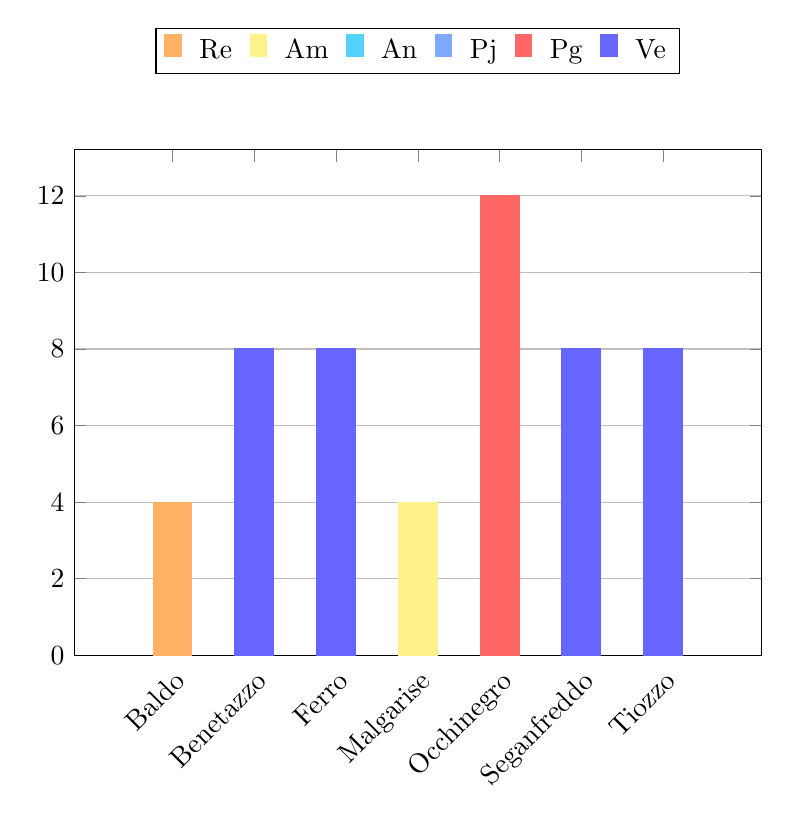
\begin{tikzpicture}
        \begin{axis}[
            width  = 0.85*\textwidth,
            height = 8cm,
            ybar stacked,
            bar width=14pt,
            ymajorgrids = true,
            symbolic x coords={Baldo, Benetazzo, Ferro, Malgarise, Occhinegro, Seganfreddo, Tiozzo},
            xtick = data,
            scaled y ticks = false,
            enlarge x limits=0.2,
            ymin=0,
            legend cell align=left,
            legend style={
                at={(0.5,1.15)},
                anchor=south,
                column sep=1ex,
                legend columns=-1
            },
            xticklabel style={rotate=45, anchor=north east, yshift=0ex, xshift=0ex},
            ]
            \addplot+[ybar, resp, fill=resp, mark=none] plot coordinates {
                (Baldo, 4)
                (Benetazzo, 0)
                (Ferro, 0)
                (Malgarise, 0)
                (Occhinegro, 0)
                (Seganfreddo, 0)
                (Tiozzo, 0)
            };
            \addplot+[ybar, amm, fill=amm, mark=none] plot coordinates {
                (Baldo, 0)
                (Benetazzo, 0)
                (Ferro, 0)
                (Malgarise, 4)
                (Occhinegro, 0)
                (Seganfreddo, 0)
                (Tiozzo, 0)
            };
            \addplot+[ybar, an, fill=an, mark=none] plot coordinates {
                (Baldo, 0)
                (Benetazzo, 0)
                (Ferro, 0)
                (Malgarise, 0)
                (Occhinegro, 0)
                (Seganfreddo, 0)
                (Tiozzo, 0)
            };
            \addplot+[ybar, pj, fill=pj, mark=none] plot coordinates {
                (Baldo, 0)
                (Benetazzo, 0)
                (Ferro, 0)
                (Malgarise, 0)
                (Occhinegro, 0)
                (Seganfreddo, 0)
                (Tiozzo, 0)
            };
            \addplot+[ybar, pg, fill=pg, mark=none] plot coordinates {
                (Baldo, 0)
                (Benetazzo, 0)
                (Ferro, 0)
                (Malgarise, 0)
                (Occhinegro, 12)
                (Seganfreddo, 0)
                (Tiozzo, 0)
            };
            \addplot+[ybar, ver, fill=ver, mark=none] plot coordinates {
                (Baldo, 0)
                (Benetazzo, 8)
                (Ferro, 8)
                (Malgarise, 0)
                (Occhinegro, 0)
                (Seganfreddo, 8)
                (Tiozzo, 8)
            };
            \legend{Re, Am, An, Pj, Pg, Ve}
        \end{axis}
    \end{tikzpicture}
    \caption{Impegno preventivo per ruolo dei membri durante il tredicesimo \href{https://7last.github.io/docs/pb/documentazione-interna/glossario\#sprint}{sprint\textsubscript{G}}}
    
\end{figure}

\newpage

%---------1_GRAFICO A TORTA-----------%
\begin{figure}[!h]
    \centering
    \begin{tikzpicture}
        \def\printonlypositive#1{\ifdim#1pt>0pt
        #1
        \fi}
        \pie[pos={8,0},radius=3.5,text=legend,
        before number=\printonlypositive,color={resp,amm,pg,ver}] {
             7.7/\href{https://7last.github.io/docs/pb/documentazione-interna/glossario\#responsabile}{Responsabile\textsubscript{G}},
             7.7/\href{https://7last.github.io/docs/pb/documentazione-interna/glossario\#amministratore}{Amministratore\textsubscript{G}},
             23.1/\href{https://7last.github.io/docs/pb/documentazione-interna/glossario\#programmatore}{Programmatore\textsubscript{G}},
             61.5/\href{https://7last.github.io/docs/pb/documentazione-interna/glossario\#verificatore}{Verificatore\textsubscript{G}}
        }
        \end{tikzpicture}
    \caption{Ripartizione in percentuale dei ruoli nel tredicesimo \href{https://7last.github.io/docs/pb/documentazione-interna/glossario\#sprint}{sprint\textsubscript{G}}}
\end{figure}

\subsubsubsection{Consuntivo}
Il collaudo con il \href{https://7last.github.io/docs/pb/documentazione-interna/glossario\#proponente}{proponente\textsubscript{G}} si è concluso con esito positivo, non c'è stata quindi la necessità di apportare modifiche al prodotto. Le attività di verifica finale della documentazione sono state completate con successo.

\subsubsubsubsection{Prospetto orario}
\begin{table}[!h]
    \centering
    \begin{tabular}{ | l | c | c | c | c | c | c | c | }
        \hline
        \textbf{} & \textbf{Re} & \textbf{Am} &\textbf{An} & \textbf{Pj} & \textbf{Pg} & \textbf{Ve} & \textbf{Totale per persona} \\
        \hline
        Baldo            &  4   &  -   &  -   &  -   &  -   &  -   &  4   \\
        Benetazzo        &  -   &  -   &  -   &  -   &  -   &  9   &  9   \\
        Ferro            &  -   &  -   &  -   &  -   &  -   & 11   & 11   \\
        Malgarise        &  -   &  5   &  -   &  -   &  -   &  -   &  5   \\
        Occhinegro       &  -   &  -   &  -   &  -   &  9   &  -   &  9   \\
        Seganfreddo      &  -   &  -   &  -   &  -   &  -   &  6   &  6   \\
        Tiozzo           &  -   &  -   &  -   &  -   &  -   &  7,5 &  7,5 \\
        \hline
        Totale per ruolo &  4   &  5   &  -   &  -   &  9   & 33,5 &  -   \\
        \hline
    \end{tabular}
    \caption{Consuntivo orario per ruolo dei membri durante il tredicesimo \href{https://7last.github.io/docs/pb/documentazione-interna/glossario\#sprint}{sprint\textsubscript{G}}}
\end{table}

\newpage
\subsubsubsubsection{Prospetto economico}
\begin{table}[!h]
    \centering
    \begin{tabular}{ | l | c | c | c | c | c | }
        \hline
        \textbf{Ruolo} & \textbf{Ore} & \textbf{Costo} & \textbf{Ore rimanenti preventivo} & \textbf{Ore rimanenti consuntivo} \\
        \hline
        \href{https://7last.github.io/docs/pb/documentazione-interna/glossario\#responsabile}{Responsabile\textsubscript{G}}     &  4   &  120,00 € &   2   &   2   \\
        \href{https://7last.github.io/docs/pb/documentazione-interna/glossario\#amministratore}{Amministratore\textsubscript{G}} &  5   &  100,00 € &  -2   &  -3   \\
        \href{https://7last.github.io/docs/pb/documentazione-interna/glossario\#analista}{Analista\textsubscript{G}}             &  0   &    0,00 € &  -8   &  -8   \\
        \href{https://7last.github.io/docs/pb/documentazione-interna/glossario\#progettista}{Progettista\textsubscript{G}}       &  0   &    0,00 € &   8   &   8   \\
        \href{https://7last.github.io/docs/pb/documentazione-interna/glossario\#programmatore}{Programmatore\textsubscript{G}}   &  9   &  135,00 € &  14   &  17   \\
        \href{https://7last.github.io/docs/pb/documentazione-interna/glossario\#verificatore}{Verificatore\textsubscript{G}}     & 33,5 &  502,50 € &   4,5 &   3   \\
        \hline
        \textbf{Totale preventivo} & 52   &  860,00 € &  18,5 &   -   \\
        \hline
        \textbf{Totale consuntivo} & 51,5 &  857,50 € &   -   &  19   \\
        \hline
    \end{tabular}
    \caption{Consuntivo economico durante il tredicesimo \href{https://7last.github.io/docs/pb/documentazione-interna/glossario\#sprint}{sprint\textsubscript{G}}}
\end{table}

\subsubsubsubsection{Rischi effettivamente occorsi e loro mitigazione}
Per questo \href{https://7last.github.io/docs/pb/documentazione-interna/glossario\#sprint}{sprint\textsubscript{G}} non si sono verificati rischi, né tra quelli preventivati né tra quelli non preventivati.

\subsubsubsection{Retrospettiva}
Il collaudo finale con il \href{https://7last.github.io/docs/pb/documentazione-interna/glossario\#proponente}{proponente\textsubscript{G}} è stato superato con successo, l'azienda si è detta estremamente soddisfatta del lavoro svolto. Abbiamo ricevuto un feedback molto positivo e alcune indicazioni per migliorare la presentazione del prodotto. Non ci sono state quindi modifiche da apportare al prodotto, permettendo al gruppo di concentrarsi sulla verifica finale della documentazione. Questo ha permesso di completare tutte le attività previste per questo \href{https://7last.github.io/docs/pb/documentazione-interna/glossario\#sprint}{sprint\textsubscript{G}} in anticipo rispetto alla data di fine prevista e di poter avanzare la propria candidatura per la revisione \href{https://7last.github.io/docs/pb/documentazione-interna/glossario\#product-baseline}{PB\textsubscript{G}} due giorni prima di quanto preventivato.
